%&preformat-disser
\RequirePackage[l2tabu,orthodox]{nag} % Раскомментировав, можно в логе получать рекомендации относительно правильного использования пакетов и предупреждения об устаревших и нерекомендуемых пакетах
% Формат А4, 14pt (ГОСТ Р 7.0.11-2011, 5.3.6)
\documentclass[a4paper,14pt,oneside,openany,oldfontcommands]{memoir}

%%%%%%%%%%%%%%%%%%%%%%%%%%%%%%%%%%%%%%%%%%%%%%%%%%%%%%%%%%%%%%%%%%%%%%%%%%%%%%%%
%%%% Файл упрощённых настроек шаблона, общих для диссертации и автореферата %%%%
%%%%%%%%%%%%%%%%%%%%%%%%%%%%%%%%%%%%%%%%%%%%%%%%%%%%%%%%%%%%%%%%%%%%%%%%%%%%%%%%

%%% Режим черновика %%%
\makeatletter
\@ifundefined{c@draft}{
  \newcounter{draft}
  \setcounter{draft}{0}  % 0 --- чистовик (максимальное соблюдение ГОСТ)
                         % 1 --- черновик (отклонения от ГОСТ, но быстрая
                         %       сборка итоговых PDF)
}{}
\makeatother

%%% Пометки в тексте %%%
\makeatletter
\@ifundefined{c@showmarkup}{
  \newcounter{showmarkup}
  \setcounter{showmarkup}{0}  % 0 --- скрыть пометки
                              % 1 --- показывать пометки
}{}
\makeatother

%%% Использование в pdflatex шрифтов не по-умолчанию %%%
\makeatletter
\@ifundefined{c@usealtfont}{
  \newcounter{usealtfont}
  \setcounter{usealtfont}{0}    % 0 --- шрифты на базе Computer Modern
                                % 1 --- использовать пакет pscyr, при его
                                %       наличии
                                % 2 --- использовать пакет XCharter, при наличии
                                %       подходящей версии
}{}
\makeatother

%%% Использование в xelatex и lualatex семейств шрифтов %%%
\makeatletter
\@ifundefined{c@fontfamily}{
  \newcounter{fontfamily}
  \setcounter{fontfamily}{0}  % 0 --- CMU семейство. Используется как fallback;
                              % 1 --- Шрифты от MS (Times New Roman и компания)
                              % 2 --- Семейство Liberation
}{}
\makeatother

%%% Библиография %%%
\makeatletter
\@ifundefined{c@bibliosel}{
  \newcounter{bibliosel}
  \setcounter{bibliosel}{1}   % 0 --- встроенная реализация с загрузкой файла
                              %       через движок bibtex8;
                              % 1 --- реализация пакетом biblatex через движок
                              %       biber
}{}
\makeatother

%%% Предкомпиляция tikz рисунков для ускорения работы %%%
\makeatletter
\@ifundefined{c@imgprecompile}{
  \newcounter{imgprecompile}
  \setcounter{imgprecompile}{0}   % 0 --- без предкомпиляции;
                                  % 1 --- пользоваться предварительно
                                  %       скомпилированными pdf вместо генерации
                                  %       заново из tikz
}{}
\makeatother
            % общие настройки шаблона
\input{common/packages}         % Пакеты общие для диссертации и автореферата
\synopsisfalse                      % Этот документ --- не автореферат
\input{Dissertation/dispackages}    % Пакеты для диссертации
\input{Dissertation/userpackages}   % Пакеты для специфических пользовательских задач

%%%%%%%%%%%%%%%%%%%%%%%%%%%%%%%%%%%%%%%%%%%%%%%%%%%%%%
%%%% Файл упрощённых настроек шаблона диссертации %%%%
%%%%%%%%%%%%%%%%%%%%%%%%%%%%%%%%%%%%%%%%%%%%%%%%%%%%%%

%%% Инициализирование переменных, не трогать!  %%%
\newcounter{intvl}
\newcounter{otstup}
\newcounter{contnumeq}
\newcounter{contnumfig}
\newcounter{contnumtab}
\newcounter{pgnum}
\newcounter{chapstyle}
\newcounter{headingdelim}
\newcounter{headingalign}
\newcounter{headingsize}
%%%%%%%%%%%%%%%%%%%%%%%%%%%%%%%%%%%%%%%%%%%%%%%%%%%%%%

%%% Область упрощённого управления оформлением %%%

%% Интервал между заголовками и между заголовком и текстом %%
% Заголовки отделяют от текста сверху и снизу
% тремя интервалами (ГОСТ Р 7.0.11-2011, 5.3.5)
\setcounter{intvl}{1}               % Коэффициент кратности к размеру шрифта

%% Отступы у заголовков в тексте %%
\setcounter{otstup}{0}              % 0 --- без отступа; 1 --- абзацный отступ

%% Нумерация формул, таблиц и рисунков %%
% Нумерация формул
\setcounter{contnumeq}{0}   % 0 --- пораздельно (во введении подряд,
                            %       без номера раздела);
                            % 1 --- сквозная нумерация по всей диссертации
% Нумерация рисунков
\setcounter{contnumfig}{0}  % 0 --- пораздельно (во введении подряд,
                            %       без номера раздела);
                            % 1 --- сквозная нумерация по всей диссертации
% Нумерация таблиц
\setcounter{contnumtab}{1}  % 0 --- пораздельно (во введении подряд,
                            %       без номера раздела);
                            % 1 --- сквозная нумерация по всей диссертации

%% Оглавление %%
\setcounter{pgnum}{1}       % 0 --- номера страниц никак не обозначены;
                            % 1 --- Стр. над номерами страниц (дважды
                            %       компилировать после изменения настройки)
\settocdepth{subsection}    % до какого уровня подразделов выносить в оглавление
\setsecnumdepth{subsection} % до какого уровня нумеровать подразделы


%% Текст и форматирование заголовков %%
\setcounter{chapstyle}{1}     % 0 --- разделы только под номером;
                              % 1 --- разделы с названием "Глава" перед номером
\setcounter{headingdelim}{1}  % 0 --- номер отделен пропуском в 1em или \quad;
                              % 1 --- номера разделов и приложений отделены
                              %       точкой с пробелом, подразделы пропуском
                              %       без точки;
                              % 2 --- номера разделов, подразделов и приложений
                              %       отделены точкой с пробелом.

%% Выравнивание заголовков в тексте %%
\setcounter{headingalign}{0}  % 0 --- по центру;
                              % 1 --- по левому краю

%% Размеры заголовков в тексте %%
\setcounter{headingsize}{0}   % 0 --- по ГОСТ, все всегда 14 пт;
                              % 1 --- пропорционально изменяющийся размер
                              %       в зависимости от базового шрифта

%% Подпись таблиц %%

% Смещение строк подписи после первой строки
\newcommand{\tabindent}{0cm}

% Тип форматирования заголовка таблицы:
% plain --- название и текст в одной строке
% split --- название и текст в разных строках
\newcommand{\tabformat}{plain}

%%% Настройки форматирования таблицы `plain`

% Выравнивание по центру подписи, состоящей из одной строки:
% true  --- выравнивать
% false --- не выравнивать
\newcommand{\tabsinglecenter}{false}

% Выравнивание подписи таблиц:
% justified   --- выравнивать как обычный текст («по ширине»)
% centering   --- выравнивать по центру
% centerlast  --- выравнивать по центру только последнюю строку
% centerfirst --- выравнивать по центру только первую строку (не рекомендуется)
% raggedleft  --- выравнивать по правому краю
% raggedright --- выравнивать по левому краю
\newcommand{\tabjust}{justified}

% Разделитель записи «Таблица #» и названия таблицы
\newcommand{\tablabelsep}{~\cyrdash\ }

%%% Настройки форматирования таблицы `split`

% Положение названия таблицы:
% \centering   --- выравнивать по центру
% \raggedleft  --- выравнивать по правому краю
% \raggedright --- выравнивать по левому краю
\newcommand{\splitformatlabel}{\raggedleft}

% Положение текста подписи:
% \centering   --- выравнивать по центру
% \raggedleft  --- выравнивать по правому краю
% \raggedright --- выравнивать по левому краю
\newcommand{\splitformattext}{\raggedright}

%% Подпись рисунков %%
%Разделитель записи «Рисунок #» и названия рисунка
\newcommand{\figlabelsep}{~\cyrdash\ }  % (ГОСТ 2.105, 4.3.1)
                                        % "--- здесь не работает

%%% Цвета гиперссылок %%%
% Latex color definitions: http://latexcolor.com/
\definecolor{linkcolor}{rgb}{0.9,0,0}
\definecolor{citecolor}{rgb}{0,0.6,0}
\definecolor{urlcolor}{rgb}{0,0,1}
%\definecolor{linkcolor}{rgb}{0,0,0} %black
%\definecolor{citecolor}{rgb}{0,0,0} %black
%\definecolor{urlcolor}{rgb}{0,0,0} %black
      % Упрощённые настройки шаблона

\input{common/newnames}         % Новые переменные, для всего проекта

%%% Основные сведения %%%
\newcommand{\thesisAuthorLastName}{\fixme{Феофанова}}
\newcommand{\thesisAuthorOtherNames}{\fixme{Мария Геннадьевна}}
\newcommand{\thesisAuthorInitials}{\fixme{И.\,О.}}
\newcommand{\thesisAuthor}             % Диссертация, ФИО автора
{%
    \texorpdfstring{% \texorpdfstring takes two arguments and uses the first for (La)TeX and the second for pdf
        \thesisAuthorLastName~\thesisAuthorOtherNames% так будет отображаться на титульном листе или в тексте, где будет использоваться переменная
    }{%
        \thesisAuthorLastName, \thesisAuthorOtherNames% эта запись для свойств pdf-файла. В таком виде, если pdf будет обработан программами для сбора библиографических сведений, будет правильно представлена фамилия.
    }
}
\newcommand{\thesisAuthorShort}        % Диссертация, ФИО автора инициалами
{\thesisAuthorInitials~\thesisAuthorLastName}
%\newcommand{\thesisUdk}                % Диссертация, УДК
%{\fixme{xxx.xxx}}
\newcommand{\thesisTitle}              % Диссертация, название
{\fixme{Верификация многопоточных структур данных и примитивов синхронизации}}
\newcommand{\thesisSpecialtyNumber}    % Диссертация, специальность, номер
{\fixme{01.03.02}}
\newcommand{\thesisSpecialtyTitle}     % Диссертация, специальность, название (название взято с сайта ВАК для примера)
{\fixme{Прикладная математика и информатика}}
%% \newcommand{\thesisSpecialtyTwoNumber} % Диссертация, вторая специальность, номер
%% {\fixme{XX.XX.XX}}
%% \newcommand{\thesisSpecialtyTwoTitle}  % Диссертация, вторая специальность, название
%% {\fixme{Теория и~методика физического воспитания, спортивной тренировки,
%% оздоровительной и~адаптивной физической культуры}}
\newcommand{\thesisDegree}             % Диссертация, ученая степень
{\fixme{кандидата физико-математических наук}}
\newcommand{\thesisDegreeShort}        % Диссертация, ученая степень, краткая запись
{\fixme{канд. физ.-мат. наук}}
\newcommand{\thesisCity}               % Диссертация, город написания диссертации
{\fixme{Город}}
\newcommand{\thesisYear}               % Диссертация, год написания диссертации
{\the\year}
\newcommand{\thesisOrganization}       % Диссертация, организация
{\fixme{Федеральное государственное автономное образовательное учреждение высшего
образования <<Длинное название образовательного учреждения <<АББРЕВИАТУРА>>}}
\newcommand{\thesisOrganizationShort}  % Диссертация, краткое название организации для доклада
{\fixme{НазУчДисРаб}}

\newcommand{\thesisInOrganization}     % Диссертация, организация в предложном падеже: Работа выполнена в ...
{\fixme{учреждении с~длинным длинным длинным длинным названием, в~котором
выполнялась данная диссертационная работа}}

%% \newcommand{\supervisorDead}{}           % Рисовать рамку вокруг фамилии
\newcommand{\supervisorFio}              % Научный руководитель, ФИО
{\fixme{Фамилия Имя Отчество}}
\newcommand{\supervisorRegalia}          % Научный руководитель, регалии
{\fixme{уч. степень, уч. звание}}
\newcommand{\supervisorFioShort}         % Научный руководитель, ФИО
{\fixme{И.\,О.~Фамилия}}
\newcommand{\supervisorRegaliaShort}     % Научный руководитель, регалии
{\fixme{уч.~ст.,~уч.~зв.}}

%% \newcommand{\supervisorTwoDead}{}        % Рисовать рамку вокруг фамилии
%% \newcommand{\supervisorTwoFio}           % Второй научный руководитель, ФИО
%% {\fixme{Фамилия Имя Отчество}}
%% \newcommand{\supervisorTwoRegalia}       % Второй научный руководитель, регалии
%% {\fixme{уч. степень, уч. звание}}
%% \newcommand{\supervisorTwoFioShort}      % Второй научный руководитель, ФИО
%% {\fixme{И.\,О.~Фамилия}}
%% \newcommand{\supervisorTwoRegaliaShort}  % Второй научный руководитель, регалии
%% {\fixme{уч.~ст.,~уч.~зв.}}

\newcommand{\opponentOneFio}           % Оппонент 1, ФИО
{\fixme{Фамилия Имя Отчество}}
\newcommand{\opponentOneRegalia}       % Оппонент 1, регалии
{\fixme{доктор физико-математических наук, профессор}}
\newcommand{\opponentOneJobPlace}      % Оппонент 1, место работы
{\fixme{Не очень длинное название для места работы}}
\newcommand{\opponentOneJobPost}       % Оппонент 1, должность
{\fixme{старший научный сотрудник}}

\newcommand{\opponentTwoFio}           % Оппонент 2, ФИО
{\fixme{Фамилия Имя Отчество}}
\newcommand{\opponentTwoRegalia}       % Оппонент 2, регалии
{\fixme{кандидат физико-математических наук}}
\newcommand{\opponentTwoJobPlace}      % Оппонент 2, место работы
{\fixme{Основное место работы c длинным длинным длинным длинным названием}}
\newcommand{\opponentTwoJobPost}       % Оппонент 2, должность
{\fixme{старший научный сотрудник}}

%% \newcommand{\opponentThreeFio}         % Оппонент 3, ФИО
%% {\fixme{Фамилия Имя Отчество}}
%% \newcommand{\opponentThreeRegalia}     % Оппонент 3, регалии
%% {\fixme{кандидат физико-математических наук}}
%% \newcommand{\opponentThreeJobPlace}    % Оппонент 3, место работы
%% {\fixme{Основное место работы c длинным длинным длинным длинным названием}}
%% \newcommand{\opponentThreeJobPost}     % Оппонент 3, должность
%% {\fixme{старший научный сотрудник}}

\newcommand{\leadingOrganizationTitle} % Ведущая организация, дополнительные строки. Удалить, чтобы не отображать в автореферате
{\fixme{Федеральное государственное бюджетное образовательное учреждение высшего
профессионального образования с~длинным длинным длинным длинным названием}}

\newcommand{\defenseDate}              % Защита, дата
{\fixme{DD mmmmmmmm YYYY~г.~в~XX часов}}
\newcommand{\defenseCouncilNumber}     % Защита, номер диссертационного совета
{\fixme{Д\,123.456.78}}
\newcommand{\defenseCouncilTitle}      % Защита, учреждение диссертационного совета
{\fixme{Название учреждения}}
\newcommand{\defenseCouncilAddress}    % Защита, адрес учреждение диссертационного совета
{\fixme{Адрес}}
\newcommand{\defenseCouncilPhone}      % Телефон для справок
{\fixme{+7~(0000)~00-00-00}}

\newcommand{\defenseSecretaryFio}      % Секретарь диссертационного совета, ФИО
{\fixme{Фамилия Имя Отчество}}
\newcommand{\defenseSecretaryRegalia}  % Секретарь диссертационного совета, регалии
{\fixme{д-р~физ.-мат. наук}}            % Для сокращений есть ГОСТы, например: ГОСТ Р 7.0.12-2011 + http://base.garant.ru/179724/#block_30000

\newcommand{\synopsisLibrary}          % Автореферат, название библиотеки
{\fixme{Название библиотеки}}
\newcommand{\synopsisDate}             % Автореферат, дата рассылки
{\fixme{DD mmmmmmmm}\the\year~года}

% To avoid conflict with beamer class use \providecommand
\providecommand{\keywords}%            % Ключевые слова для метаданных PDF диссертации и автореферата
{}
             % Основные сведения
%%% Кодировки и шрифты %%%

%\begin{comment}
\ifxetexorluatex
    \setmainlanguage[babelshorthands=true]{russian}    % Язык по-умолчанию русский с поддержкой приятных команд пакета babel
    \setotherlanguage{english}                         % Дополнительный язык = английский (в американской вариации по-умолчанию)

    % Проверка существования шрифтов. Недоступна в pdflatex
    \ifnumequal{\value{fontfamily}}{1}{
        \IfFontExistsTF{Times New Roman}{}{\setcounter{fontfamily}{0}}
    }{}
    \ifnumequal{\value{fontfamily}}{2}{
        \IfFontExistsTF{LiberationSerif}{}{\setcounter{fontfamily}{0}}
    }{}

    \ifnumequal{\value{fontfamily}}{0}{                    % Семейство шрифтов CMU. Используется как fallback
        \setmonofont{CMU Typewriter Text}                  % моноширинный шрифт
        \newfontfamily\cyrillicfonttt{Courier New} % моноширинный шрифт для кириллицы
        \defaultfontfeatures{Ligatures=TeX}                % стандартные лигатуры TeX, замены нескольких дефисов на тире и т. п. Настройки моноширинного шрифта должны идти до этой строки, чтобы при врезках кода программ в коде не применялись лигатуры и замены дефисов
        \setmainfont{CMU Serif}                            % Шрифт с засечками
        \newfontfamily\cyrillicfont{CMU Serif}             % Шрифт с засечками для кириллицы
        \setsansfont{CMU Sans Serif}                       % Шрифт без засечек
        \newfontfamily\cyrillicfontsf{CMU Sans Serif}      % Шрифт без засечек для кириллицы
    }

    \ifnumequal{\value{fontfamily}}{1}{                    % Семейство MS шрифтов
        \setmonofont{Courier New}                          % моноширинный шрифт
        \newfontfamily\cyrillicfonttt{Courier New}         % моноширинный шрифт для кириллицы
        \defaultfontfeatures{Ligatures=TeX}                % стандартные лигатуры TeX, замены нескольких дефисов на тире и т. п. Настройки моноширинного шрифта должны идти до этой строки, чтобы при врезках кода программ в коде не применялись лигатуры и замены дефисов
        \setmainfont{Times New Roman}                      % Шрифт с засечками
        \newfontfamily\cyrillicfont{Times New Roman}       % Шрифт с засечками для кириллицы
        \setsansfont{Arial}                                % Шрифт без засечек
        \newfontfamily\cyrillicfontsf{Arial}               % Шрифт без засечек для кириллицы
    }

    \ifnumequal{\value{fontfamily}}{2}{                    % Семейство шрифтов Liberation (https://pagure.io/liberation-fonts)
        \setmonofont{LiberationMono}[Scale=0.87] % моноширинный шрифт
        \newfontfamily\cyrillicfonttt{LiberationMono}[     % моноширинный шрифт для кириллицы
            Scale=0.87]
        \defaultfontfeatures{Ligatures=TeX}                % стандартные лигатуры TeX, замены нескольких дефисов на тире и т. п. Настройки моноширинного шрифта должны идти до этой строки, чтобы при врезках кода программ в коде не применялись лигатуры и замены дефисов
        \setmainfont{LiberationSerif}                      % Шрифт с засечками
        \newfontfamily\cyrillicfont{LiberationSerif}       % Шрифт с засечками для кириллицы
        \setsansfont{LiberationSans}                       % Шрифт без засечек
        \newfontfamily\cyrillicfontsf{LiberationSans}      % Шрифт без засечек для кириллицы
    }

\else
    \ifnumequal{\value{usealtfont}}{1}{% Используется pscyr, при наличии
        \IfFileExists{pscyr.sty}{\renewcommand{\rmdefault}{ftm}}{}
    }{}
\fi
%\end{comment}            % Определение шрифтов (частичное)
%%% Шаблон %%%
\DeclareRobustCommand{\fixme}{\textcolor{red}}  % решаем проблему превращения
                                % названия цвета в результате \MakeUppercase,
                                % http://tex.stackexchange.com/a/187930,
                                % \DeclareRobustCommand protects \fixme
                                % from expanding inside \MakeUppercase
\AtBeginDocument{%
    \setlength{\parindent}{1.25cm}                   % Абзацный отступ. Должен быть одинаковым по всему тексту и равен пяти знакам (ГОСТ Р 7.0.11-2011, 5.3.7).
}

%%% Таблицы %%%
\DeclareCaptionLabelSeparator{tabsep}{\tablabelsep} % нумерация таблиц
\DeclareCaptionFormat{split}{\splitformatlabel#1\par\splitformattext#3}

\captionsetup[table]{
        format=\tabformat,                % формат подписи (plain|hang)
        font=normal,                      % нормальные размер, цвет, стиль шрифта
        skip=.0pt,                        % отбивка под подписью
        parskip=.0pt,                     % отбивка между параграфами подписи
        position=above,                   % положение подписи
        justification=\tabjust,           % центровка
        indent=\tabindent,                % смещение строк после первой
        labelsep=tabsep,                  % разделитель
        singlelinecheck=\tabsinglecenter, % не выравнивать по центру, если умещается в одну строку
}

%%% Рисунки %%%
\DeclareCaptionLabelSeparator{figsep}{\figlabelsep} % нумерация рисунков

\captionsetup[figure]{
        format=plain,                     % формат подписи (plain|hang)
        font=normal,                      % нормальные размер, цвет, стиль шрифта
        skip=.0pt,                        % отбивка под подписью
        parskip=.0pt,                     % отбивка между параграфами подписи
        position=below,                   % положение подписи
        singlelinecheck=true,             % выравнивание по центру, если умещается в одну строку
        justification=centerlast,         % центровка
        labelsep=figsep,                  % разделитель
}

%%% Подписи подрисунков %%%
\DeclareCaptionSubType{figure}
\renewcommand\thesubfigure{\asbuk{subfigure}} % нумерация подрисунков
\ifsynopsis
\DeclareCaptionFont{norm}{\fontsize{10pt}{11pt}\selectfont}
\newcommand{\subfigureskip}{2.pt}
\else
\DeclareCaptionFont{norm}{\fontsize{14pt}{16pt}\selectfont}
\newcommand{\subfigureskip}{0.pt}
\fi

\captionsetup[subfloat]{
        labelfont=norm,                 % нормальный размер подписей подрисунков
        textfont=norm,                  % нормальный размер подписей подрисунков
        labelsep=space,                 % разделитель
        labelformat=brace,              % одна скобка справа от номера
        justification=centering,        % центровка
        singlelinecheck=true,           % выравнивание по центру, если умещается в одну строку
        skip=\subfigureskip,            % отбивка над подписью
        parskip=.0pt,                   % отбивка между параграфами подписи
        position=below,                 % положение подписи
}

%%% Настройки гиперссылок %%%
\ifluatex
    \hypersetup{
        unicode,                % Unicode encoded PDF strings
    }
\fi

\hypersetup{
    linktocpage=true,           % ссылки с номера страницы в оглавлении, списке таблиц и списке рисунков
    linktoc=all,                % both the section and page part are links
%    pdfpagelabels=false,        % set PDF page labels (true|false)
    plainpages=false,           % Forces page anchors to be named by the Arabic form  of the page number, rather than the formatted form
    colorlinks,                 % ссылки отображаются раскрашенным текстом, а не раскрашенным прямоугольником, вокруг текста
    linkcolor={blue},      % цвет ссылок типа ref, eqref и подобных
    citecolor={citecolor},      % цвет ссылок-цитат
    urlcolor={urlcolor},        % цвет гиперссылок
%    hidelinks,                  % Hide links (removing color and border)
    pdftitle={\thesisTitle},    % Заголовок
    pdfauthor={\thesisAuthor},  % Автор
    pdfsubject={\thesisSpecialtyNumber\ \thesisSpecialtyTitle},      % Тема
%    pdfcreator={Создатель},     % Создатель, Приложение
%    pdfproducer={Производитель},% Производитель, Производитель PDF
    pdfkeywords={\keywords},    % Ключевые слова
    pdflang={ru},
}
\ifnumequal{\value{draft}}{1}{% Черновик
    \hypersetup{
        draft,
    }
}{}

\let \olditemize=\itemize \let \endolditemize=\enditemize \renewenvironment{itemize}{\olditemize \itemsep0.5em}{\endolditemize}

\let \oldenumerate=\enumerate \let \endoldenumerate=\endenumerate \renewenvironment{enumerate}{\oldenumerate \itemsep0.5em}{\endoldenumerate}

%%% Списки %%%
% Используем короткое тире (endash) для ненумерованных списков (ГОСТ 2.105-95, пункт 4.1.7, требует дефиса, но так лучше смотрится)
%\renewcommand{\labelitemi}{\normalfont\bfseries{--}}

% Перечисление строчными буквами латинского алфавита (ГОСТ 2.105-95, 4.1.7)
%\renewcommand{\theenumi}{\alph{enumi}}
%\renewcommand{\labelenumi}{\theenumi)}

% Перечисление строчными буквами русского алфавита (ГОСТ 2.105-95, 4.1.7)
\makeatletter
\AddEnumerateCounter{\asbuk}{\russian@alph}{щ}      % Управляем списками/перечислениями через пакет enumitem, а он 'не знает' про asbuk, потому 'учим' его
\makeatother
%\renewcommand{\theenumi}{\asbuk{enumi}} %первый уровень нумерации
%\renewcommand{\labelenumi}{\theenumi)} %первый уровень нумерации
\renewcommand{\theenumii}{\asbuk{enumii}} %второй уровень нумерации
\renewcommand{\labelenumii}{\theenumii)} %второй уровень нумерации
\renewcommand{\theenumiii}{\arabic{enumiii}} %третий уровень нумерации
\renewcommand{\labelenumiii}{\theenumiii)} %третий уровень нумерации

\setlist{nosep,%                                    % Единый стиль для всех списков (пакет enumitem), без дополнительных интервалов.
    labelindent=\parindent,leftmargin=*%            % Каждый пункт, подпункт и перечисление записывают с абзацного отступа (ГОСТ 2.105-95, 4.1.8)
}

%%% Правильная нумерация приложений, рисунков и формул %%%
%% По ГОСТ 2.105, п. 4.3.8 Приложения обозначают заглавными буквами русского алфавита,
%% начиная с А, за исключением букв Ё, З, Й, О, Ч, Ь, Ы, Ъ.
%% Здесь также переделаны все нумерации русскими буквами.
\ifxetexorluatex
    \makeatletter
    \def\russian@Alph#1{\ifcase#1\or
       А\or Б\or В\or Г\or Д\or Е\or Ж\or
       И\or К\or Л\or М\or Н\or
       П\or Р\or С\or Т\or У\or Ф\or Х\or
       Ц\or Ш\or Щ\or Э\or Ю\or Я\else\xpg@ill@value{#1}{russian@Alph}\fi}
    \def\russian@alph#1{\ifcase#1\or
       а\or б\or в\or г\or д\or е\or ж\or
       и\or к\or л\or м\or н\or
       п\or р\or с\or т\or у\or ф\or х\or
       ц\or ш\or щ\or э\or ю\or я\else\xpg@ill@value{#1}{russian@alph}\fi}
    \def\cyr@Alph#1{\ifcase#1\or
        А\or Б\or В\or Г\or Д\or Е\or Ж\or
        И\or К\or Л\or М\or Н\or
        П\or Р\or С\or Т\or У\or Ф\or Х\or
        Ц\or Ш\or Щ\or Э\or Ю\or Я\else\xpg@ill@value{#1}{cyr@Alph}\fi}
    \def\cyr@alph#1{\ifcase#1\or
        а\or б\or в\or г\or д\or е\or ж\or
        и\or к\or л\or м\or н\or
        п\or р\or с\or т\or у\or ф\or х\or
        ц\or ш\or щ\or э\or ю\or я\else\xpg@ill@value{#1}{cyr@alph}\fi}
    \makeatother
\else
    \makeatletter
    \if@uni@ode
      \def\russian@Alph#1{\ifcase#1\or
        А\or Б\or В\or Г\or Д\or Е\or Ж\or
        И\or К\or Л\or М\or Н\or
        П\or Р\or С\or Т\or У\or Ф\or Х\or
        Ц\or Ш\or Щ\or Э\or Ю\or Я\else\@ctrerr\fi}
    \else
      \def\russian@Alph#1{\ifcase#1\or
        \CYRA\or\CYRB\or\CYRV\or\CYRG\or\CYRD\or\CYRE\or\CYRZH\or
        \CYRI\or\CYRK\or\CYRL\or\CYRM\or\CYRN\or
        \CYRP\or\CYRR\or\CYRS\or\CYRT\or\CYRU\or\CYRF\or\CYRH\or
        \CYRC\or\CYRSH\or\CYRSHCH\or\CYREREV\or\CYRYU\or
        \CYRYA\else\@ctrerr\fi}
    \fi
    \if@uni@ode
      \def\russian@alph#1{\ifcase#1\or
        а\or б\or в\or г\or д\or е\or ж\or
        и\or к\or л\or м\or н\or
        п\or р\or с\or т\or у\or ф\or х\or
        ц\or ш\or щ\or э\or ю\or я\else\@ctrerr\fi}
    \else
      \def\russian@alph#1{\ifcase#1\or
        \cyra\or\cyrb\or\cyrv\or\cyrg\or\cyrd\or\cyre\or\cyrzh\or
        \cyri\or\cyrk\or\cyrl\or\cyrm\or\cyrn\or
        \cyrp\or\cyrr\or\cyrs\or\cyrt\or\cyru\or\cyrf\or\cyrh\or
        \cyrc\or\cyrsh\or\cyrshch\or\cyrerev\or\cyryu\or
        \cyrya\else\@ctrerr\fi}
    \fi
    \makeatother
\fi

%%% Команды рецензирования %%%
\ifboolexpr{ (test {\ifnumequal{\value{draft}}{1}}) or (test {\ifnumequal{\value{showmarkup}}{1}})}{
        \newrobustcmd{\todo}[1]{\textcolor{red}{#1}}
        \newrobustcmd{\note}[2][]{\ifstrempty{#1}{#2}{\textcolor{#1}{#2}}}
        \newenvironment{commentbox}[1][]%
        {\ifstrempty{#1}{}{\color{#1}}}%
        {}
}{
        \newrobustcmd{\todo}[1]{}
        \newrobustcmd{\note}[2][]{}
        \excludecomment{commentbox}
}

           % Стили общие для диссертации и автореферата
%%% Переопределение именований, если иначе не сработает %%%
%\gappto\captionsrussian{
%    \renewcommand{\chaptername}{Глава}
%    \renewcommand{\appendixname}{Приложение} % (ГОСТ Р 7.0.11-2011, 5.7)
%}

%%% Изображения %%%
\graphicspath{{images/}{Dissertation/images/}}         % Пути к изображениям

%%% Интервалы %%%
%% По ГОСТ Р 7.0.11-2011, пункту 5.3.6 требуется полуторный интервал
%% Реализация средствами класса (на основе setspace) ближе к типографской классике.
%% И правит сразу и в таблицах (если со звёздочкой)
%\DoubleSpacing*     % Двойной интервал
\OnehalfSpacing*    % Полуторный интервал
%\setSpacing{1.42}   % Полуторный интервал, подобный Ворду (возможно, стоит включать вместе с предыдущей строкой)

%%% Макет страницы %%%
% Выставляем значения полей (ГОСТ 7.0.11-2011, 5.3.7)
\geometry{a4paper, top=2cm, bottom=2cm, left=3cm, right=1.5cm, nofoot, nomarginpar} %, heightrounded, showframe
\setlength{\topskip}{0pt}   %размер дополнительного верхнего поля
\setlength{\footskip}{35pt} % снимет warning, согласно https://tex.stackexchange.com/a/334346

%%% Выравнивание и переносы %%%
%% http://tex.stackexchange.com/questions/241343/what-is-the-meaning-of-fussy-sloppy-emergencystretch-tolerance-hbadness
%% http://www.latex-community.org/forum/viewtopic.php?p=70342#p70342
\tolerance 1414
\hbadness 1414
\emergencystretch 1.5em % В случае проблем регулировать в первую очередь
\hfuzz 0.3pt
\vfuzz \hfuzz
%\raggedbottom
%\sloppy                 % Избавляемся от переполнений
\clubpenalty=10000      % Запрещаем разрыв страницы после первой строки абзаца
\widowpenalty=10000     % Запрещаем разрыв страницы после последней строки абзаца
\brokenpenalty=4991     % Ограничение на разрыв страницы, если строка заканчивается переносом

%%% Блок управления параметрами для выравнивания заголовков в тексте %%%
\newlength{\otstuplen}
\setlength{\otstuplen}{\theotstup\parindent}
\ifnumequal{\value{headingalign}}{0}{% выравнивание заголовков в тексте
    \newcommand{\hdngalign}{\centering}                % по центру
    \newcommand{\hdngaligni}{}% по центру
    \setlength{\otstuplen}{0pt}
}{%
    \newcommand{\hdngalign}{}                 % по левому краю
    \newcommand{\hdngaligni}{\hspace{\otstuplen}}      % по левому краю
} % В обоих случаях вроде бы без переноса, как и надо (ГОСТ Р 7.0.11-2011, 5.3.5)

%%% Оглавление %%%
\renewcommand{\cftchapterdotsep}{\cftdotsep}                % отбивка точками до номера страницы начала главы/раздела

%% Переносить слова в заголовке не допускается (ГОСТ Р 7.0.11-2011, 5.3.5). Заголовки в оглавлении должны точно повторять заголовки в тексте (ГОСТ Р 7.0.11-2011, 5.2.3). Прямого указания на запрет переносов в оглавлении нет, но по той же логике невнесения искажений в смысл, лучше в оглавлении не переносить:
\setrmarg{2.55em plus1fil}                             %To have the (sectional) titles in the ToC, etc., typeset ragged right with no hyphenation
\renewcommand{\cftchapterpagefont}{\normalfont}        % нежирные номера страниц у глав в оглавлении
\renewcommand{\cftchapterleader}{\cftdotfill{\cftchapterdotsep}}% нежирные точки до номеров страниц у глав в оглавлении
%\renewcommand{\cftchapterfont}{}                       % нежирные названия глав в оглавлении

\ifnumgreater{\value{headingdelim}}{0}{%
    \renewcommand\cftchapteraftersnum{.\space}       % добавляет точку с пробелом после номера раздела в оглавлении
}{}
\ifnumgreater{\value{headingdelim}}{1}{%
    \renewcommand\cftsectionaftersnum{.\space}       % добавляет точку с пробелом после номера подраздела в оглавлении
    \renewcommand\cftsubsectionaftersnum{.\space}    % добавляет точку с пробелом после номера подподраздела в оглавлении
    \renewcommand\cftsubsubsectionaftersnum{.\space} % добавляет точку с пробелом после номера подподподраздела в оглавлении
    \AfterEndPreamble{% без этого polyglossia сама всё переопределяет
        \setsecnumformat{\csname the#1\endcsname.\space}
    }
}{%
    \AfterEndPreamble{% без этого polyglossia сама всё переопределяет
        \setsecnumformat{\csname the#1\endcsname\quad}
    }
}

\renewcommand*{\cftappendixname}{\appendixname\space} % Слово Приложение в оглавлении

%%% Колонтитулы %%%
% Порядковый номер страницы печатают на середине верхнего поля страницы (ГОСТ Р 7.0.11-2011, 5.3.8)
\makeevenhead{plain}{}{}{}
\makeoddhead{plain}{}{}{}
\makeevenfoot{plain}{}{\thepage}{}
\makeoddfoot{plain}{}{\thepage}{}
\pagestyle{plain}

%%% добавить Стр. над номерами страниц в оглавлении
%%% http://tex.stackexchange.com/a/306950
\newif\ifendTOC

\newcommand*{\tocheader}{
\ifnumequal{\value{pgnum}}{1}{%
    \ifendTOC\else\hbox to \linewidth%
      {\noindent{}~\hfill{Стр.}}\par%
      \ifnumless{\value{page}}{3}{}{%
        \vspace{0.5\onelineskip}
      }
      \afterpage{\tocheader}
    \fi%
}{}%
}%

%%% Оформление заголовков глав, разделов, подразделов %%%
%% Работа должна быть выполнена ... размером шрифта 12-14 пунктов (ГОСТ Р 7.0.11-2011, 5.3.8). То есть не должно быть надписей шрифтом более 14. Так и поставим.
%% Эти установки будут давать одинаковый результат независимо от выбора базовым шрифтом 12 пт или 14 пт
\newcommand{\basegostsectionfont}{\fontsize{14pt}{16pt}\selectfont\bfseries}

\makechapterstyle{thesisgost}{%
    \chapterstyle{default}
    \setlength{\beforechapskip}{0pt}
    \setlength{\midchapskip}{0pt}
    \setlength{\afterchapskip}{\theintvl\curtextsize}
    \renewcommand*{\chapnamefont}{\basegostsectionfont}
    \renewcommand*{\chapnumfont}{\basegostsectionfont}
    \renewcommand*{\chaptitlefont}{\basegostsectionfont}
    \renewcommand*{\chapterheadstart}{}
    \ifnumgreater{\value{headingdelim}}{0}{%
        \renewcommand*{\afterchapternum}{.\space}   % добавляет точку с пробелом после номера раздела
    }{%
        \renewcommand*{\afterchapternum}{\quad}     % добавляет \quad после номера раздела
    }
    \renewcommand*{\printchapternum}{\hdngaligni\hdngalign\chapnumfont \thechapter}
    \renewcommand*{\printchaptername}{}
    \renewcommand*{\printchapternonum}{\hdngaligni\hdngalign}
}

\makeatletter
\makechapterstyle{thesisgostchapname}{%
    \chapterstyle{thesisgost}
    \renewcommand*{\printchapternum}{\chapnumfont \thechapter}
    \renewcommand*{\printchaptername}{\hdngaligni\hdngalign\chapnamefont \@chapapp} %
}
\makeatother

\chapterstyle{thesisgost}

\setsecheadstyle{\basegostsectionfont\hdngalign}
\setsecindent{\otstuplen}

\setsubsecheadstyle{\basegostsectionfont\hdngalign}
\setsubsecindent{\otstuplen}

\setsubsubsecheadstyle{\basegostsectionfont\hdngalign}
\setsubsubsecindent{\otstuplen}

\sethangfrom{\noindent #1} %все заголовки подразделов центрируются с учетом номера, как block

\ifnumequal{\value{chapstyle}}{1}{%
    \chapterstyle{thesisgostchapname}
    \renewcommand*{\cftchaptername}{\chaptername\space} % будет вписано слово Глава перед каждым номером раздела в оглавлении
}{}%

%%% Интервалы между заголовками
\setbeforesecskip{\theintvl\curtextsize}% Заголовки отделяют от текста сверху и снизу тремя интервалами (ГОСТ Р 7.0.11-2011, 5.3.5).
\setaftersecskip{\theintvl\curtextsize}
\setbeforesubsecskip{\theintvl\curtextsize}
\setaftersubsecskip{\theintvl\curtextsize}
\setbeforesubsubsecskip{\theintvl\curtextsize}
\setaftersubsubsecskip{\theintvl\curtextsize}

%%% Вертикальные интервалы глав (\chapter) в оглавлении как и у заголовков
% раскомментировать следующие 2
% \setlength{\cftbeforechapterskip}{0pt plus 0pt}   % ИЛИ эти 2 строки из учебника
% \renewcommand*{\insertchapterspace}{}
% или эту  
% \renewcommand*{\cftbeforechapterskip}{0em}       


%%% Блок дополнительного управления размерами заголовков
\ifnumequal{\value{headingsize}}{1}{% Пропорциональные заголовки и базовый шрифт 14 пт
    \renewcommand{\basegostsectionfont}{\large\bfseries}
    \renewcommand*{\chapnamefont}{\Large\bfseries}
    \renewcommand*{\chapnumfont}{\Large\bfseries}
    \renewcommand*{\chaptitlefont}{\Large\bfseries}
}{}

%%% Счётчики %%%

%% Упрощённые настройки шаблона диссертации: нумерация формул, таблиц, рисунков
\ifnumequal{\value{contnumeq}}{1}{%
    \counterwithout{equation}{chapter} % Убираем связанность номера формулы с номером главы/раздела
}{}
\ifnumequal{\value{contnumfig}}{1}{%
    \counterwithout{figure}{chapter}   % Убираем связанность номера рисунка с номером главы/раздела
}{}
\ifnumequal{\value{contnumtab}}{1}{%
    \counterwithout{table}{chapter}    % Убираем связанность номера таблицы с номером главы/раздела
}{}


%%http://www.linux.org.ru/forum/general/6993203#comment-6994589 (используется totcount)
\makeatletter
\def\formbytotal#1#2#3#4#5{%
    \newcount\@c
    \@c\totvalue{#1}\relax
    \newcount\@last
    \newcount\@pnul
    \@last\@c\relax
    \divide\@last 10
    \@pnul\@last\relax
    \divide\@pnul 10
    \multiply\@pnul-10
    \advance\@pnul\@last
    \multiply\@last-10
    \advance\@last\@c
    \total{#1}~#2%
    \ifnum\@pnul=1#5\else%
    \ifcase\@last#5\or#3\or#4\or#4\or#4\else#5\fi
    \fi
}
\makeatother

\AtBeginDocument{
%% регистрируем счётчики в системе totcounter
    \regtotcounter{totalcount@figure}
    \regtotcounter{totalcount@table}       % Если иным способом поставить в преамбуле то ошибка в числе таблиц
    \regtotcounter{TotPages}               % Если иным способом поставить в преамбуле то ошибка в числе страниц
}

\setcounter{page}{2}

\setlength{\parskip}{6pt}

  % Стили для диссертации
\input{Dissertation/userstyles} % Стили для специфических пользовательских задач

%%% Библиография. Выбор движка для реализации %%%
% Здесь только проверка установленного ключа. Сама настройка выбора движка
% размещена в common/setup.tex
\ifnumequal{\value{bibliosel}}{0}{%
    \input{biblio/predefined}   % Встроенная реализация с загрузкой файла через движок bibtex8
}{
    \input{biblio/biblatex}     % Реализация пакетом biblatex через движок biber
}

% Вывести информацию о выбранных опциях в лог сборки
\typeout{Selected options:}
\typeout{Draft mode: \arabic{draft}}
\typeout{Font: \arabic{fontfamily}}
\typeout{AltFont: \arabic{usealtfont}}
\typeout{Bibliography backend: \arabic{bibliosel}}
\typeout{Precompile images: \arabic{imgprecompile}}
% Вывести информацию о версиях используемых библиотек в лог сборки
\listfiles

%%% Управление компиляцией отдельных частей диссертации %%%
% Необходимо сначала иметь полностью скомпилированный документ, чтобы все
% промежуточные файлы были в наличии
% Затем, для вывода отдельных частей можно воспользоваться командой \includeonly
% Ниже примеры использования команды:
%
%\includeonly{Dissertation/part2}
%\includeonly{Dissertation/contents,Dissertation/appendix,Dissertation/conclusion}
%
% Если все команды закомментированы, то документ будет выведен в PDF файл полностью

\usepackage{mdframed}

\usepackage{minted}

%\surroundwithmdframed{minted}

%\RecustomVerbatimEnvironment{Verbatim}{BVerbatim}{}

%\renewcommand{\figurename}{Listing}

\newfontfamily\codeubuntu{Ubuntu Mono}[NFSSFamily=CodeUbuntu]

\usemintedstyle{vs}
\setminted[]{tabsize=2, fontfamily=CodeUbuntu, fontsize=\small, frame=lines, linenos, breaklines}
%\setmintedinline[c++]{style=bw}
\setmintedinline[]{fontsize=auto}

\renewcommand{\textfraction}{0.05} 

\usepackage{float}

\makeatletter
\renewcommand{\fps@figure}{H}
\renewcommand{\fps@table}{H}
\renewcommand{\fps@listing}{H}
\makeatother


\usepackage{xcolor}

\usepackage{multicol}

\usepackage{graphicx}

\usepackage{changepage}

\usepackage{caption}

\lstset{
	basicstyle=\fontsize{5}{5}\selectfont\ttfamily,
	escapeinside={<@}{@>},
	numbers=none,
    frame=single,
}

\usepackage{fancyvrb}

\makeatletter
\newcommand{\iftoggleverb}[1]{%
  \ifcsdef{etb@tgl@#1}
    {\csname etb@tgl@#1\endcsname\iftrue\iffalse}
    {\etb@noglobal\etb@err@notoggle{#1}\iffalse}%
}
\makeatother

\newtoggle{pics}
\toggletrue{pics}
%\togglefalse{pics}

\renewcommand\listingscaption{Листинг}

\usepackage{graphbox}

\hypersetup{breaklinks=true}

\let\clsCenter\Center\let\clsendCenter\endCenter
\let\Center\undefined\let\endCenter\undefined
\usepackage{ragged2e}
\let\Center\clsCenter
\let\endCenter\clsendCenter

\usepackage{numprint}
\npthousandsep{\,}

\newcommand{\CC}{C\nolinebreak\hspace{-.05em}\raisebox{.4ex}{\tiny\bf+}\nolinebreak\hspace{-.10em}\raisebox{.4ex}{\tiny\bf+}}

\usepackage{makecell}

\begin{document}
	
\input{common/renames}                 % Переопределение именований

%%% Структура диссертации (ГОСТ Р 7.0.11-2011, 4)
%\include{Dissertation/title}           % Титульный лист


\chapter*{Аннотация}

Исполнение многопоточной программы по своей природе недетерминированно, а значит стандартных методик тестирования для верификации многопоточного кода недостаточно, требуются специальные техники: fault injection и model checking.

Целью данной работы было изучить основные методы верификации конкурентного кода, выявить их недостатки и реализовать model checker, который совместил бы преимущества обоих подходов: (как fault injection) проверял бы не модель, а код на \CC, и (как model checking) перебирал бы все достижимые из теста состояния исполнения.

В работе мы опишем реализацию разработанного model checker-а и продемонстрируем его работоспособность на двух нетривиальных примерах: lock-free аллокаторе и фреймворке экзекьюторов.



% Оглавление (ГОСТ Р 7.0.11-2011, 5.2)
\ifdefmacro{\microtypesetup}{\microtypesetup{protrusion=false}}{} % не рекомендуется применять пакет микротипографики к автоматически генерируемому оглавлению
{
  \hypersetup{linkcolor=black}
  \tableofcontents*
}
%\tableofcontents*
\addtocontents{toc}{\protect\tocheader}
\endTOCtrue
\ifdefmacro{\microtypesetup}{\microtypesetup{protrusion=true}}{}        % Оглавление


\ifnumequal{\value{contnumfig}}{1}{}{\counterwithout{figure}{chapter}}
\ifnumequal{\value{contnumtab}}{1}{}{\counterwithout{table}{chapter}}


\chapter{Введение}\label{ch:ch1}

Данная работа посвящена верификации конкурентного кода.

Опыт показывает, что даже тщательно изученный конкурентный код может скрывать в себе ошибки:

“There is a rather large body of sad experience to indicate that a concurrent program can withstand very careful scrutiny without revealing its errors.” \autocite{Liveness}

Ошибки в конкурентном коде могут быть длинными, требующими определенного порядка действий, и в рабочей среде воспроизводиться крайне редко в силу своей недетерминированной природы. 

Поэтому критически важно иметь инструменты, которые будут помогать разработчику находить, понимать и устранять такие ошибки.

В этой главе мы сформулируем задачу верификации конкурентного кода, разберем преимущества и недостатки существующих подходов, и определим цели работы.

\section{Задача верификации}

\emph{Верификация программы} – это проверка соответствия программы предъявленным к ней требованиям \autocite{Intro}.

Нас будут интересовать программы, состоящие из нескольких потоков, взаимодействующих друг с другом через разделяемую память и синхронизирующие к ней доступ с помощью атомиков, мьютексов и условных переменных. Такие программы порождают \emph{конкурентные исполнения}, которые могут быть описаны в модели чередования потоков.

Еще точнее, мы хотим верифицировать не сами многопоточные программы (которые могут быть сколь угодно большими и сложными), а изолированные примитивы синхронизации, конкурентные структуры данных и базовые инфраструктурные компоненты. На практике весь нетривиальный конкурентный код (а вместе с ними и нетривиальные конкурентные баги) изолирован именно в подобных компонентах.

Примеры примитивов синхронизации: мьютексы, спинлоки, read-write локи, семафоры и барьеры.

Примеры конкурентных объектов: lock-free структуры данных (стек, очередь, хеш-таблица).

Примеры инфраструктурных компонентов:

\begin{itemize}

\item	Экзекьюторы для асинхронного исполнения задач (пулы потоков и декораторы над ними).

\item	Аллокаторы.
\end{itemize}

Требования формулируются в виде \emph{свойств}. В случае конкурентных объектов нас будут интересовать свойства, которые выполняются или нарушаются на отдельных исполнениях. Эти свойства можно разделить на два больших класса:

\begin{itemize}
\item	\emph{Safety (безопасность)} – никогда не случится ничего плохого.

\item	\emph{Liveness (живучесть)} – когда-нибудь случится нечто хорошее.
\end{itemize}

Это неформальные определения \autocite{Proving}, строгие формулировки приведены в \autocite{SafetyLiveness}.

Примеры safety-свойств:

\begin{itemize}
\item	\emph{Mutual exclusion} – два потока не могут одновременно находиться в критической секции.

\item	Память, отданная под узел lock-free стека, не может быть в то же время доступна для аллокации.
\end{itemize} 

Все эти свойства – \emph{инварианты} – утверждения про мгновенное состояние исполнения.

Примеры liveness-свойств:

\begin{itemize}

\item	\emph{Deadlock freedom} – если несколько потоков хотят захватить свободный мьютекс, то какой-нибудь из них в итоге войдет в критическую секцию.

\item	\emph{Starvation freedom} – все потоки когда-нибудь получат доступ к ресурсу.

\end{itemize}



\section{Подходы}

Детерминированных тестов для верификации конкурентных примитивов недостаточно: планировщик операционной системы недетерминированно переключает потоки, поэтому один и тот же код порождает несколько возможных вариантов исполнения.

Два основных подхода к верификации конкурентного кода – \emph{fault injection} и \emph{model checking}.


\subsection{Fault Injection}

Подход fault injection состоит в следующем: для примитива синхронизации или конкурентной структуры данных пишется \emph{стресс-тест} и в его исполнение недетерминированно внедряются \emph{сбои}: перепланирование (\mintinline{c++}{yield}), пауза (\mintinline{c++}{sleep}) или парковка потока. 

Также при контроле над средой исполнения сбои можно внедрять непосредственно в планировщик: рандомизировать run queue или очереди ожидания в примитивах синхронизации. Этот подход реализован в планировщике языка Go в режиме поиска гонок \autocite{Go}.

Fault injection – это механизм ускорения времени: в сравнении с обычным исполнением под управлением планировщика операционной системы мы перебираем больше нетривиальных сценариев за меньшее время.

Fault injection повышает вероятность нарушения инварианта в исполнении стресс-теста, но все же не может перебрать все возможные исполнения, а значит не может гарантировать корректность реализации тестируемого объекта.


\subsection{Model Checking}

Альтернативный подход – model checking – состоит в переборе всех возможных исполнений конкурентного кода. 

Для model checking-а пишется формальная \emph{спецификация}, которая состоит из

\begin{itemize}
\item	описания конкурентного объекта,

\item	теста для него и

\item	набора свойств.
\end{itemize}

Спецификация задает направленный \emph{граф состояний}, вершинами в котором являются все состояния исполнения, достижимые при исполнении теста, а дуги соответствуют атомарным операциям. Пути в этом графе называются \emph{траекториями}.

\emph{Model checker} по спецификации строит этот граф и проверяет на его состояниях или в общем случае путях (траекториях) заданные пользователем свойства. 

Если свойство нарушилось, то model checker предъявляет соответствующую этому нарушению траекторию: путь для safety-свойств и цикл для liveness-cвойств.

У fault injection-а и model checking-а схожие цели – исследовать граф состояний теста. Но, в отличие от fault injection-а, который перебирает отдельные траектории в графе состояний, model checking анализирует \emph{все} исполнения теста.

%\pagebreak

\subsection{+Cal / TLC}

Интерес индустрии к model checking-у начался после статьи “Use of Formal Methods at Amazon Web Services” \autocite{AWS}. В ней инженеры AWS рассказали про свой опыт верификации многопоточных структур данных и распределенных алгоритмов, лежащих в основе облачной инфраструктуры Amazon:
 
\begin{figure}
	\centerfloat{
		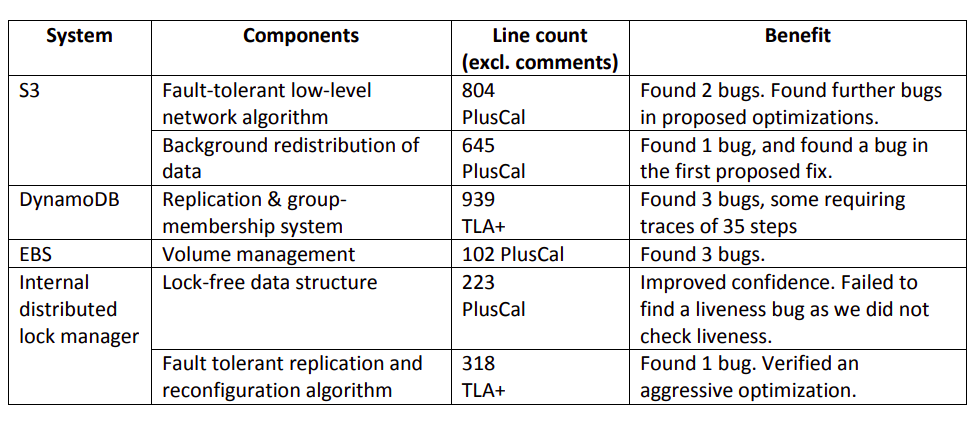
\includegraphics[scale=0.4]{aws}
	}
	\caption{Применение TLA+ / +Cal в AWS.}\label{fig:aws}
\end{figure}

Для верификации инженеры AWS выбрали языки спецификации TLA+ / +Cal и model checker TLC \autocite{Tla}. В работе мы будем говорить про +Cal, так как именно этот язык используется для спецификации многопоточного кода.

Спецификация на +Cal представляет собой псевдокод, напоминающий, в зависимости от выбранного варианта синтаксиса, код на языке C или Pascal. В качестве примера приведем фрагмент спецификации lock-free стека, написанного на C-синтаксисе языка +Cal:

\begin{figure}
\centerfloat{
\begin{tabular}{p{0.5\textwidth} p{0.5\textwidth}}
	\centering
	\vspace{0pt} 
    
    \fbox{\parbox[t][.28\textheight]{0.48\textwidth}{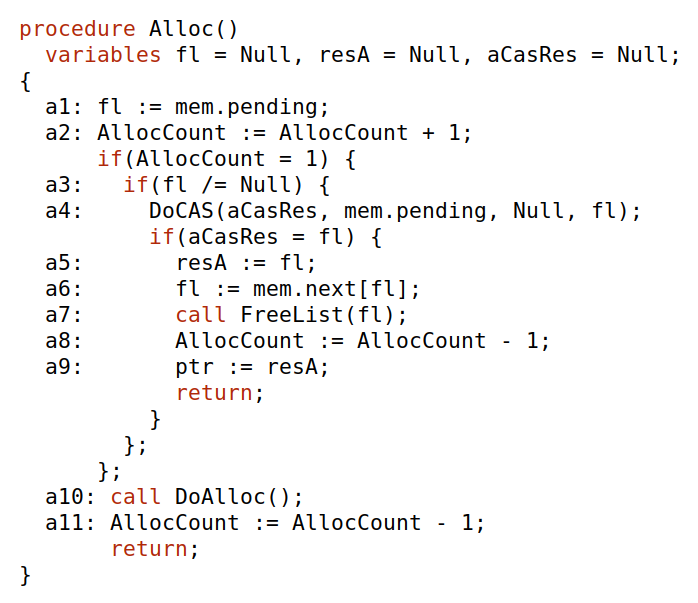
\includegraphics[width=0.48\textwidth]{specalloc}}}
    
	 &
	\vspace{0pt} 
    
    \fbox{\parbox[t][.28\textheight]{0.48\textwidth}{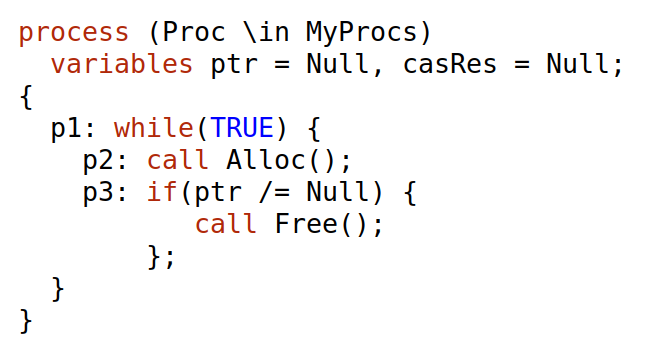
\includegraphics[width=0.35\textwidth]{spectest}}}
    
	\\
	\hfil Фрагмент алгоритма & \hfil Тест
\end{tabular}
}
\bigskip
\caption{Фрагмент спецификации lock-free стека на +Cal.}
\end{figure}



Этот псевдокод автоматически транслируется в формальный язык TLA+ и проверяется model checker-ом TLC. 

На сегодняшний день +Cal / TLC широко используется в индустрии для верификации конкурентных и распределенных алгоритмов: 

\begin{itemize}
	
\item	Спецификация конкурентных алгоритмов помогла найти баги в ядре Linux \autocite{LinuxConf} \autocite{LinuxSpec}.

\item	В Яндексе с помощью +Cal / TLC воспроизвели сценарий ABA в lock-free кеше аллокатора памяти \autocite{YaAlloc} и верифицировали исправленную версию алгоритма \autocite{YaSpec}.

\item	В Microsoft использовали +Cal для спецификации моделей согласованности распределенной базы данных CosmosDB \autocite{MsSpec}.

\item	В CockroachLabs использовали +Cal / TLC для верификации алгоритма коммита распределенных транзакций в базе данных CockroachDB \autocite{CockroachSpec}.

\end{itemize}


\subsection{Недостатки +Cal / TLC}

Хотя +Cal / TLC и являются де-факто стандартным языком спецификации / model checker-ом в индустрии, этот инструмент имеет ряд серьезных недостатков.

Самый главный и очевидный: +Cal – не язык программирования. Верифицируемый код приходится транслировать в псевдокод, а недостающие сущности – моделировать:

\begin{itemize}

\item   В +Cal нет таких сущностей как куча и указатели, их приходится заменять массивами и индексами:

\begin{figure}
	\centerfloat{
		\fbox{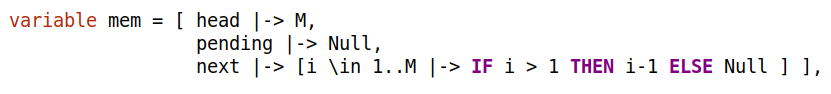
\includegraphics[scale=0.5]{calmem}}
	}
	\bigskip
	\caption{Моделирование памяти стека в +Cal.}\label{fig:calmem}
\end{figure}

\item   В +Сal нет атомарных операций. Атомарность определяется \emph{метками (labels)}: все действия в пределах одной метки являются атомарным шагом с точки зрения model checker-а. 

\end{itemize}

В результате такой трансляции можно упустить сценарий конкуренции, в котором нарушается инвариант.

Например, Лесли Лэмпорт, автор TLA+ и +Cal, в статье про проверку многопоточного алгоритма на +Cal признается, как случайно опустил метку и проверял фактически другой алгоритм: “... There is an amusing footnote to this story. After doing the checking, I noticed that I had inadvertently omitted a label from the pushRight operation, letting one atomic action access two shared variables.” \autocite{LamportPLuscal}

Траектории, найденные TLC, трудно читать. +Сal перед проверкой транслируется в спецификацию на TLA+, фактически – логический “ассемблер”, и TLC работает уже с этим “ассемблером”. В результате траектория состоит из низкоуровневого снимка стеков вызовов, служебных регистров (\mintinline{c++}{pc}) и всех переменных, в нем много нерелевантной информации. От исходного кода в траектории остаются только названия меток.

\begin{figure}
	\centerfloat{
		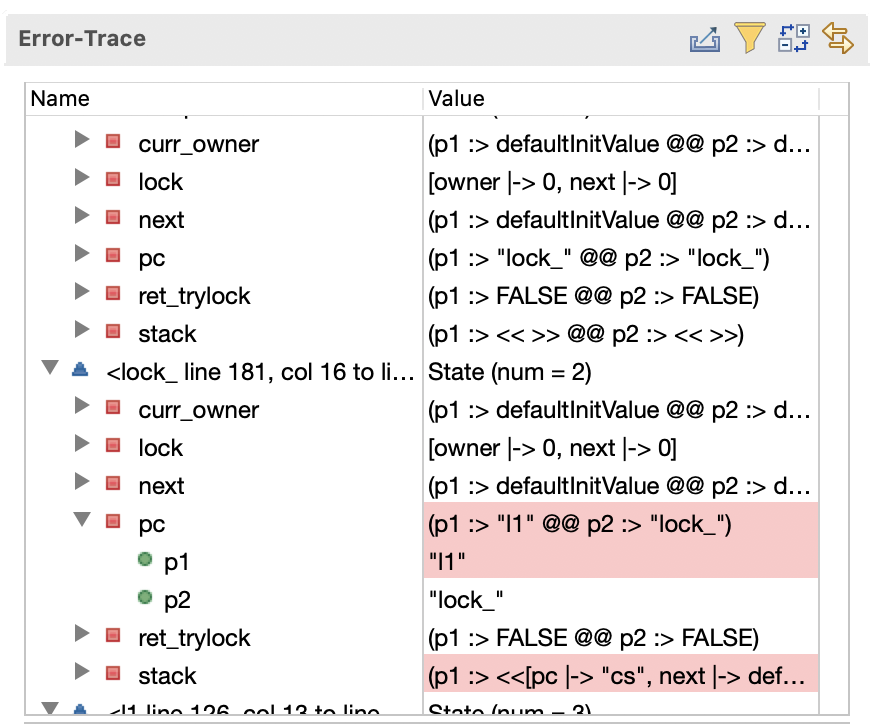
\includegraphics[scale=0.3]{caltrace}
	}
	\bigskip
	\caption{Траектория в TLA+ Toolbox.}\label{fig:caltrace}
\end{figure}

Наконец, у +Cal / TLC довольно высокий порог входа: пользователю придется изучить новый язык и разобраться с основами темпоральной логики и TLA+.

\section{Цели работы}

Для перебора всех состояний исполнения не обязательно писать на псевдокоде. Вполне можно выполнять этот перебор и над настоящим кодом. 

Цель работы – реализовать model checker, который:

\begin{itemize}
\item	{[}\emph{как +Cal / TLC}{]} Перебирает все исполнения теста.

\item	{[}\emph{как +Cal / TLC}{]} Печатает траекторию, которая приводит к нарушению инварианта. 

\item	{[}\emph{как fault injection}{]} Проверяет код на \CC, а не его модель.

\item	Показывает настоящие стектрейсы и состояния локальных переменных. 

\item	Не требует от пользователя специальных знаний в области model checking-а.
\end{itemize}

Ограничения:

\begin{itemize}
\item	Мы будем проверять не программы, а изолированные примитивы синхронизации или базовые инфраструктурные компоненты.

\item	Мы будем верифицировать только выполнение инвариантов (которые в коде тестов выражаются в виде assert-ов), и оставляем за границами работы liveness-свойства (например, livelock-и) и более сложные safety-свойства.

\item	Мы будем “разветвлять” исполнение только в точках обращения к примитивам синхронизации / атомикам. Мотивация будет приведена во второй главе работы. 

\item	Мы будем поддерживать только последовательно согласованные программы и игнорировать слабые модели памяти (\mintinline{c++}{memory_order} $\ne$ \mintinline{c++}{sec_cst}).
\end{itemize}


\section{План работы}

Во второй главе мы разберем устройство реализованного model checker-а: как перебирать исполнения многопоточного кода, как бороться с экспоненциальным ростом числа состояний, какие трудности возникают при проверке кода на \CC. 

В третьей главе мы продемонстрируем работоспособность model checker-а на двух нетривиальных примерах: lock-free аллокаторе и фреймворке экзекьюторов.

В четвертой главе мы посмотрим на инструменты, которые позволяют пользователю управлять атомарностью и отсекать ветки при переборе, выражать недетерминизм в коде теста, детализировать траекторию. 



\chapter{Model checker}\label{ch:ch2}

В этой главе мы разберем устройство реализованного \autocite{CheckerRepo} model checker-а.

\section{Управление исполнением}

Чтобы перебирать состояния исполнения, нужно:

\begin{itemize}
\item	делать снимки текущего состояния исполнения в точках обращения к примитивам синхронизации / атомикам;

\item	восстанавливать это состояние из снимка;

\item	управлять очередностью исполнения потоков (управлять планировщиком).
\end{itemize}

Для этого будем пользоваться \emph{файберами} – кооперативными потоками, реализованными в пространстве пользователя. По сути, мы продублируем в пространстве пользователя всю механику исполнения из ядра операционной системы: управление очередью исполнения и очередями ожидания в примитивах синхронизации, процедуру переключения контекста исполнения и т.п.

Файберы исполняются в одном потоке операционной системы, что исключает влияние на моделируемое исполнение недетерминизма системного планировщика.

Файбер хранит в себе:

\begin{itemize}

\item	Стек – заранее аллоцированный регион памяти.

\item	Контекст – callee-saved регистры, instruction pointer, stack pointer (имеет смысл только для остановленного файбера).

\item	Enum состояния: файбер готов исполняться (\mintinline{c++}{runnable}) / заснул в очереди ядра (\mintinline{c++}{suspended}) / завершил исполнение (\mintinline{c++}{terminated}).

\item	Пользовательскую функцию.

\end{itemize}

Переключение контекста файбера реализовано на ассемблере и состоит из следующих шагов:

\begin{enumerate}

\item	На стек файбера сохраняется контекст исполнения: значения callee-saved регистров.

\item	\mintinline{c++}{rsp} текущего файбера фиксируется в поле файбера для восстановления контекста в будущем.

\item	\mintinline{c++}{rsp} переключается на стек нового файбера.

\item	С нового стека восстанавливается контекст (значения callee-saved регистров).

\end{enumerate}

Таким образом, в файбере в поле с контекстом фактически хранится лишь указатель \mintinline{c++}{rsp}, остальные регистры хранятся на стеке.

\textbf{Замечание:} в работе мы будем использовать термин \emph{файберы}, когда речь идет о реализации model checker-а, и \emph{потоки}, когда речь идет о наблюдаемом поведении теста / свойствах конкурентных исполнений. Пользователь model checker-а работает только с потоками (через объект \mintinline{text}{thread}) и никаких файберов не наблюдает.


\section{Снимки состояния}

Состояние исполнения образовано:

\begin{itemize}
\item	состоянием каждого файбера (стек, регистры, enum состояния, исполняемая функция);

\item	состоянием динамической памяти (кучи).
\end{itemize}

Снимок состояния делается в контексте model checker-а, т.е. в момент, когда ни один из файберов не исполняется.

Снимок регистров отдельно делать не нужно: при переключении контекста нужные регистры сохраняются на вершину стека остановленного файбера, так что достаточно сохранять только сами стеки.

Сохраняется только использованная часть стека – до адреса \mintinline{c++}{rsp} (он доступен через сохраненный контекст исполнения).

Между стеками файберов / стеком и кучей могут быть ссылки, про которые model checker ничего не знает (один файбер захватывает мьютекс, который расположен на стеке другого файбера / файбер создает \mintinline{c++}{shared_ptr} на объект), поэтому память для стеков и кучи выделяется в model checker-е один раз, и при каждом восстановлении снимка стеки и куча восстанавливаются по своим прежним адресам. 

Все аллокации в тесте перехватываются, и если аллокация выполняется непосредственно пользовательским кодом (а не model checker-ом), то ее обрабатывает специальный аллокатор. Аллокатор поддерживает свободные блоки в интрузивном односвязном списке внутри заранее выделенной арены памяти. Снимок аллокатора – это использованный диапазон арены и два указателя: на голову списка свободных блоков и на границу использованного префикса арены.

Служебные аллокации, выполняемые в контексте файбера (например, при запуске нового потока-файбера), отделяются от пользовательских аллокаций с помощью расставленных в библиотеке \mintinline{c++}{AllocationGuard}-ов. \mintinline{c++}{AllocationGuard} выключает аллокатор model checker-а в области своей жизни.

Итого, снимок состояния в model checker-е образован:

\begin{itemize}
\item	стеком, enum-ом состояния и исполняемой функцией каждого файбера;

\item	снимком кучи.
\end{itemize}

\begin{figure}
	\centerfloat{
		
		
					\begin{tabular}{c c c}
						%\centering 
						\fbox{{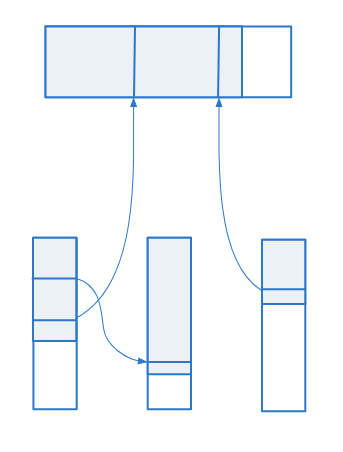
\includegraphics[align=c,width=0.35\textwidth]{snap1}}}
						&
						${\Longrightarrow}$
						& \fbox{{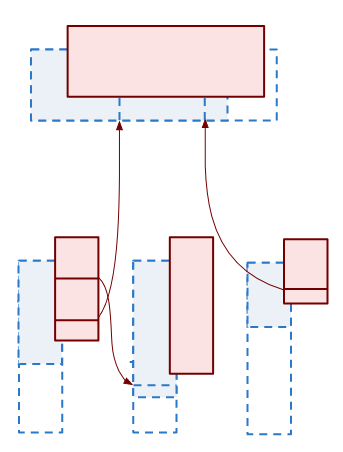
\includegraphics[align=c,width=0.35\textwidth]{snap2}}}
						\\
						\hfil Память (куча и стеки) & & \hfil Снимок
					\end{tabular}
			
	}
	\bigskip
	\caption{Снятие снимка состояния.}
\end{figure}

\section{Перебор исполнений}

Чтобы находить кратчайшие нарушения инвариантов, будем обходить граф состояний исполнения поиском в ширину. Граф не материализуется в памяти явно, вместо этого мы умеем из каждого состояния получать все смежные с ним.

\subsection{Обход графа состояний}

Посмотрим, как model checker перебирает исполнения теста.

Ключевой объект model checker-а – это очередь состояний, продолжения которых еще нужно посетить, фронт обхода в ширину. 

На старте model checker создает первый файбер, который будет исполнять код теста, и кладет снимок начального состояния в очередь.

Теперь посмотрим на цикл обхода графа состояний. На очередной итерации model checker достает из очереди снимок состояния, перебирает все файберы, которые в этом состоянии могут продолжить работу, и для каждого из них исполняет один \emph{шаг} (\mintinline{c++}{Step}). 

\iftoggleverb{pics}

\begin{figure}
	\centerfloat{
		\fbox{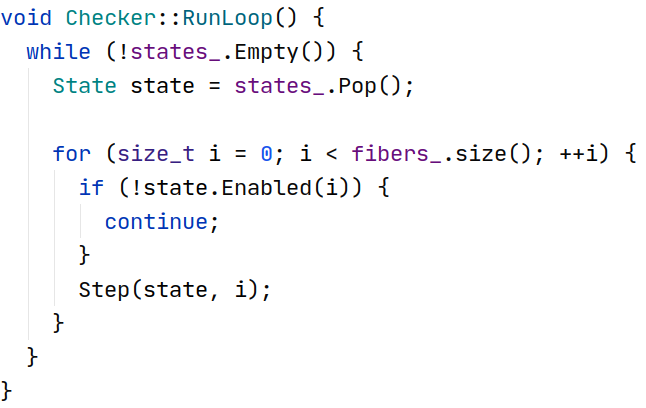
\includegraphics[scale=0.5]{runloop}}
	}
	\bigskip
	\caption{Цикл model checker-а.}\label{fig:runloop}
\end{figure}

\else

\begin{listing}
	\centering
	
	\begin{minted}{c++}
void Checker::RunLoop() {
	while (!states_.Empty()) {
		State state = states_.Pop();

		const size_t fiber_count = fibers_.size();
		for (size_t i = 0; i < fiber_count; ++i) {
			if (!state.Enabled(i)) {
				continue;
			}
			Step(state, i);
		}
	}
}
	\end{minted}
	\caption{Цикл model checker-а.}
	\label{loop}
\end{listing}

\fi

Перебор \mintinline{c++}{runnable} файберов для каждого снимка – это и есть ветвление исполнения, по сути мы рандомизируем run queue в планировщике.

\subsection{Шаг исполнения}

Шаг исполнения файбера заключен между точками обращения к разделяемым объектам (примитивам синхронизации / атомикам / аллокатору памяти) и реализуется парой служебных функций \mintinline{c++}{Step} / \mintinline{c++}{Fork}.

Начинается шаг с вызова функции \mintinline{c++}{Step}: в контексте model checker-а из снимка восстанавливается состояние исполнения (куча и стеки накладываются на соответствующие регионы памяти), затем контекст переключается на выбранный файбер (который ранее остановился в вызове \mintinline{c++}{Fork}).

Далее файбер исполняется до тех пор, пока не встретит следующий вызов функции \mintinline{c++}{Fork}.

\iftoggleverb{pics}

\begin{figure}
	\centerfloat{
		\fbox{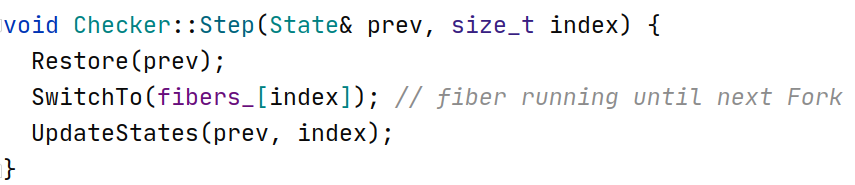
\includegraphics[scale=0.4]{step}}
	}
	\bigskip
	\caption{Шаг файбера (\mintinline{c++}{Step}).}\label{fig:step}
\end{figure}

\else

\begin{listing}
	\centering
	
	\begin{minted}{c++}
    
void Checker::Step(State& prev, size_t index) {
  Restore(prev);
  SwitchTo(fibers_[index]);
  // fiber running until next Fork...
  UpdateStates(prev, index);
}

	\end{minted}
	\caption{Шаг файбера (\mintinline{c++}{Step}).}
	\label{step}
\end{listing}

\fi

Вызов \mintinline{c++}{Fork} – точка ветвления, в ней может произойти переключение на произвольный \mintinline{c++}{runnable} файбер. Вызов \mintinline{c++}{Fork} переключает контекст файбера на контекст model checker-а, тот делает снимок состояния исполнения и помещает его в очередь поиска в ширину.

\begin{figure}
	\centerfloat{
		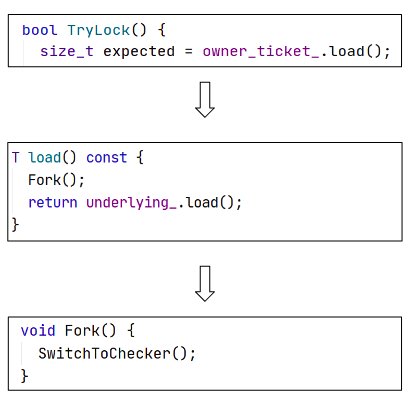
\includegraphics[scale=0.5]{forkblack}
	}
	\caption{Развилка в коде (вызов \mintinline{c++}{Fork}).}\label{fig:fork}
\end{figure}

\subsection{Точки ветвления}

Будем предполагать, что реализация верифицируемого конкурентного объекта не содержит data race-ов, т.е. проверяемый тест – программа, \emph{свободная от гонок (data-race-free)}. 

Если программа свободна от гонок, то потоки в ней не могут наблюдать относительный порядок действий между точками синхронизации в другом потоке (т.е. между обращениями к атомикам, мьютексам и другим объектам, через которые реализуется отношение synchronizes-with).

Это наблюдение упрощает перебор model checker-а: ветвления исполнения (вызовы \mintinline{c++}{Fork}) можно встраивать только при обращении к объектам, через которые осуществляется синхронизация.

Чтобы перехватывать обращения к атомикам, мьютексам и условным переменным и ветвить в них исполнения, мы пишем собственные версии этих примитивов и требуем от пользователя model checker-а, чтобы он использовал их вместо стандартных (для этого в проверяемом коде придется заменить пространство имен с \mintinline{c++}{std} на пространство имен библиотеки model checker-а, на данный момент это \mintinline{c++}{twist::stdlike}).

\iftoggleverb{pics}

\begin{figure}
	\centerfloat{
		\fbox{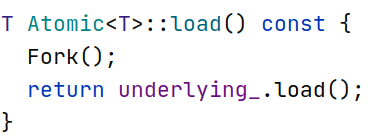
\includegraphics[scale=0.5]{load}}
	}
	\bigskip
	\caption{Собственная реализация \mintinline{c++}{load} у атомика.}\label{fig:lock}
\end{figure}

\else

\begin{listing}
	\centering
	
	\begin{minted}{c++}
    
void Mutex::Lock() {
  Fork();
  while (locked_) {
    wait_queue_.Park();
  }
  locked_ = true;
}

	\end{minted}
	\caption{Реализация метода lock у мьютекса.}
	\label{lock}
\end{listing}

\fi

Аналогично, для перехвата динамических аллокаций мы переопределяем операторы \mintinline{text}{new} / \mintinline{text}{delete}: если находимся в контексте пользовательского кода, вызываем аллокатор model checker-а, иначе – \mintinline{c++}{malloc} / \mintinline{c++}{free}.

\subsection{Run queue / Wait queue}

Model checker – не планировщик, в нем нет явной очереди \mintinline{c++}{runnable} файберов (run queue), для каждого снимка запускается каждый \mintinline{c++}{runnable} файбер. 

Аналогично мы поступаем с блокирующими примитивами синхронизации, которые внутри имеют очереди ожидания (мьютексы, условные переменные): 

Явно такие очереди не моделируются, вместо этого в каждом файбере хранится адрес очереди, в которой он заснул. Когда, например, мьютекс в \mintinline{c++}{unlock} будит один из заблокированных на нем файберов, model checker создает сразу несколько веток исполнения – по ветке на каждый файбер, у которого в поле адреса хранится текущая очередь.

В планировщике Go \autocite{Go} при поиске гонок происходит рандомизация очередей ожидания и исполнения. У нас же случайность трансформируется в перебор всех возможных исполнений.


\subsection{Очередь во внешней памяти}

С ростом исследуемой глубины исполнения количество состояний будет расти экспоненциально, фронт поиска в ширину быстро станет огромным (в одном из тестов размер фронта достигал десятков миллионов состояний) и перестанет помещаться в оперативную память.

Поэтому очередь для поиска в ширину в model checker-е реализована во внешней памяти. Вот как она устроена:

Все состояния в очереди делятся на две непрерывные группы (фронта):

\begin{enumerate}

\item	\emph{Старый фронт} – состояния наименьшей глубины ($d$). 

\item	\emph{Новый фронт} – состояния, полученные из старого фронта (глубины $d+1$). 

\end{enumerate}
	
Пока не исчерпался старый фронт, в очереди не могут появиться состояния глубины $d+2$.
 
Будем поддерживать по файлу на каждый из двух фронтов: один для чтения старого фронта, другой – для записи нового. При смене глубины старый фронт отбрасывается, а новый – переходит в старый. 

Model checker не работает с файлами напрямую, вместо этого он использует специальный аллокатор, который работает с аренами памяти, отображенными в файлы с помощью \mintinline{c++}{mmap}-а.

Максимальный перерасход внешней памяти (в два раза) происходит при смене глубины. Но почти всегда издержки компенсируются (если следующий фронт произведет хотя бы в два раза больше состояний).


\subsection{Повторные состояния}

Чтобы не посещать одни и те же состояния повторно, model checker хеширует снимки состояний и не помещает снимок в очередь, если его хеш уже встречался ранее.

Хеширование неизбежно ведет к потере информации, поэтому model checker может упустить состояния, если произойдет \emph{коллизия} – ситуация, когда двум состояниям ставится в соответствие один хеш. 

TLC аналогичным образом использует хеширование состояний. Кроме того, он оценивает вероятность коллизии и дает возможность пользователю перезапустить перебор с другой хеш-функцией:

“TLC saves only 64-bit fingerprints (hashes) of the reachable states that it finds, not the complete states.  If two different reachable states have the same fingerprint, a situation called a collision, TLC may not find all reachable states.  At the end of a run, TLC prints estimates of how likely it was that a collision occurred.” \autocite{TlcOptions}

\begin{figure}
	\centerfloat{
		\fbox{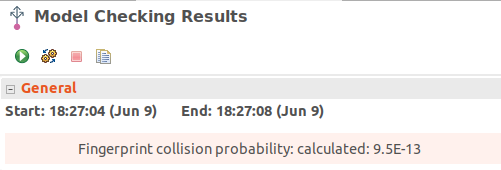
\includegraphics[scale=0.5]{fingerprint}}
	}
	\bigskip
	\caption{Вероятность коллизии, показанная в TLA+ Toolbox.}\label{fig:fingerprint}
\end{figure}

Но вероятность коллизии невелика, и на практике хеширование не мешает model checker-у находить баги, зато сильно ускоряет проверку. 

Для хеширования model checker использует FNV-функцию \autocite{Fnv}: она быстрая и обобщается на комбинирование хешей (что удобно для хеширования состояний исполнения).
  
При хешировании участков памяти (стеки, куча) помогает развертка цикла \autocite{FasterHash}. Развертка разрывает зависимость следующей итерации цикла от предыдущей, и процессор (фактически, конвейер для инструкций) выполнит такие итерации параллельно.

\section{Симметрия}

Любой model checker сталкивается с проблемой \emph{state space explosion}. Даже если разветвляться только перед обращениями к разделяемым объектам, количество состояний будет расти экспоненциально с ростом количества атомиков / потоков. 

Но если разные потоки исполняют один и тот же код (что ожидаемо для теста мьютекса или конкурентной структуры данных), то некоторые состояния могут быть \emph{симметричны} – сводиться одно к другому с помощью перенумерации потоков. 

Чтобы учесть симметрию, model checker \emph{канонизирует} состояние: стирает со стеков зависимости от адреса конкретного потока (например, ссылки на свой же стек заменяет относительными отступами). Получившиеся стеки хешируются по отдельности, сортируются и комбинируются в один результирующий хеш.

TLC тоже предоставляет такую оптимизацию и обобщает это наблюдение до симметрии множеств \autocite{Symmetry}.

\section{Проверка инвариантов}

Цель model checker-а – найти нарушение инварианта в некотором исполнении теста или убедиться в отсутствии таких нарушений во всех исполнениях.

Есть две вариации инвариантов:

\begin{itemize}

\item	Локальный инвариант – аналог обычного assert-а, задается в коде теста макросом \mintinline{c++}{CHECKER_ASSERT(condition)}. Проверка выполняется в контексте пользовательского потока. Если \mintinline{c++}{condition} не выполнен, то управление передается model checker-у, и тот сообщает об ошибке. 

\item	Глобальный инвариант – произвольный предикат на разделяемом состоянии. Инвариант проверяется в контексте model checker-а: проверка запускается на каждое новое состояние в исполнении и происходит атомарно (с отключенными \mintinline{c++}{Fork}-ами). Глобальный инвариант задается в начале теста с помощью \mintinline{c++}{AddInvariant(predicate)}.

\end{itemize}

Для проверки взаимного исключения в мьютексе удобнее поставить \mintinline{c++}{CHECKER_ASSERT} в критической секции: 

\iftoggleverb{pics}

\begin{figure}
	\centerfloat{
		\fbox{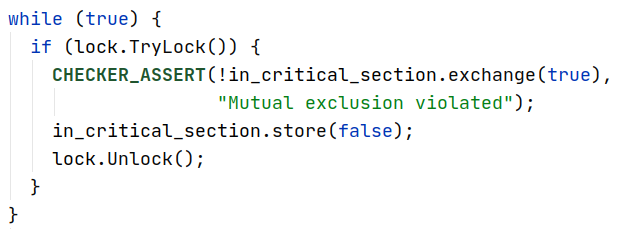
\includegraphics[scale=0.5]{checkerassert}}
	}
	\bigskip
	\caption{Локальный инвариант.}
\end{figure}

\else

\begin{listing}
	\centering
	
	\begin{minted}{c++}
    
while (true) {
  if (lock.TryLock()) {
    CHECKER_ASSERT(!in_critical_section.exchange(true), "Mutual exclusion violated");
    in_critical_section.store(false);
    lock.Unlock();
  }
}

	\end{minted}
	\caption{Локальный инвариант.}
	\label{local}
\end{listing}

\fi

Но инварианты lock-free стека уже трудно проверить локально, для него удобнее использовать глобальный вариант (например, он может проверять, что каждый узел стека действительно аллоцирован (см. \ref{app:A3})):

\iftoggleverb{pics}

\begin{figure}
	\centerfloat{
		\fbox{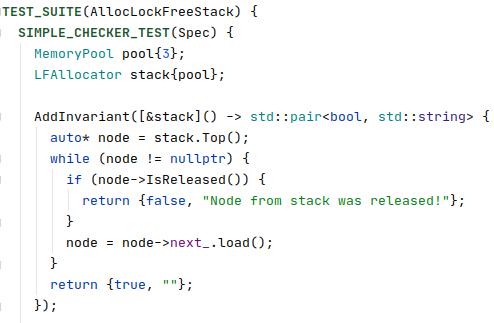
\includegraphics[scale=0.7]{globalassert}}
	}
	\bigskip
	\caption{Глобальный инвариант.}
\end{figure}

\else

\begin{listing}
	\centering
	
	\begin{minted}{c++}

TEST_SUITE(AllocLockFreeStack) {
  SIMPLE_CHECKER_TEST(Spec) {
    MemoryPool pool{3};
    LFAllocator stack{pool};
        
    AddInvariant([&stack]() -> std::pair<bool, std::string> {
      // check every node of stack...
      // validation failed -> return {false, report}
    });
	
    // test code...
  }
}
	\end{minted}
	\caption{Глобальный инвариант.}
	\label{localinv}
\end{listing}

\fi

В model checker-е реализован глобальный служебный инвариант – проверка \emph{взаимной блокировки (deadlock)}. Взаимная блокировка с точки зрения model checker-а – достижимое состояние, в котором еще есть живые потоки, но нет ни одного потока, готового исполняться (т.е. в состоянии \mintinline{c++}{runnable}). Как и TLC, model checker проверяет этот инвариант по умолчанию.  


\section{Печать траектории}

Если при проверке теста model checker находит состояние, в котором нарушается пользовательский или служебный инвариант, то он завершает перебор и печатает найденную траекторию. Пример найденной траектории приведен в приложении \ref{app:trace}.

Проверка инварианта и печать траектории разделены между двумя режимами сборки теста: \mintinline{c++}{Check} и \mintinline{c++}{Trace}.

В режиме \mintinline{c++}{Check} model checker обходит граф состояний исполнения и с каждым снимком состояния хранит траекторию, которая привела к этому состоянию. Траектория детерминирует выбор очередного потока в каждой развилке исполнения и кодируется последовательностью индексов потоков: на $i$-ой позиции записан номер потока, который был выбран на $i$-ом вызове \mintinline{c++}{Fork}. В случае нарушения инварианта найденная траектория сохраняется на диск.

В режиме \mintinline{c++}{Trace} model checker считывает с диска найденную в первом режиме траекторию и проигрывает ее, показывая для каждой развилки разделяемое состояние, стеки потоков и локальные переменные.  

Траектория разделена на секции (\emph{runs}), каждая секция – непрерывный фрагмент исполнения одного потока, который ограничен переключением контекста / стартом потока (слева) / завершением потока (справа).

Каждая секция показывает состояние потока в нескольких временных точках: снимки состояния до и после исполнения секции, и промежуточные снимки в точках обращения к атомикам / примитивам синхронизации / аллокатору памяти.

Для каждого шага в секции печатается:

\begin{itemize}
\item	Разделяемое состояние. Model checker не знает, как устроено и как печатать разделяемое состояние, пользователь пишет процедуру печати самостоятельно и через \mintinline{c++}{PrintState} в начале теста передает ее model checker-у.

\begin{figure}
	\centerfloat{
		\fbox{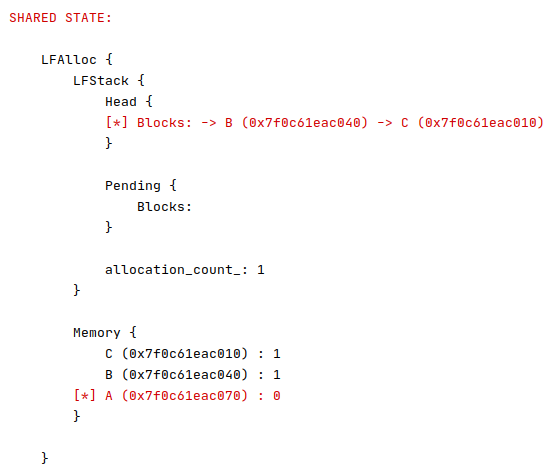
\includegraphics[scale=0.5]{sharedstate}}
	}
	\bigskip
	\caption{Разделяемое состояние.}
\end{figure}

\item	Стектрейсы потока. Стектрейсы собираются с помощью библиотеки \mintinline{c++}{backward-cpp} \autocite{Backward}. Служебные фрагменты стектрейса (вызовы внутри model checker-а), код стандартной и сторонних библиотек фильтруется.

\item	Локальные переменные. В точке, где мы хотим снять значения локальных переменных, мы вызываем \mintinline{c++}{fork} и из дочернего процесса присоединяемся отладчиком (\mintinline{c++}{gdb}) к родительскому. В планах – использовать программный интерфейс \mintinline{c++}{lldb} вместо запуска дебаггера.

\begin{figure}
	\centerfloat{
		\fbox{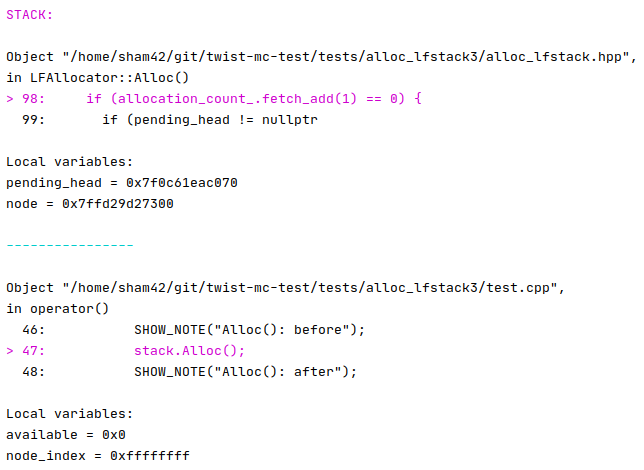
\includegraphics[scale=0.5]{stacklocals}}
	}
	\bigskip
	\caption{Стектрейсы и локальные переменные.}
\end{figure}

\item	Заметки о служебных событиях во время исполнения потока. Добавляются с помощью макроса \mintinline{c++}{SHOW_NOTE}.

\begin{figure}
	\centerfloat{
		\fbox{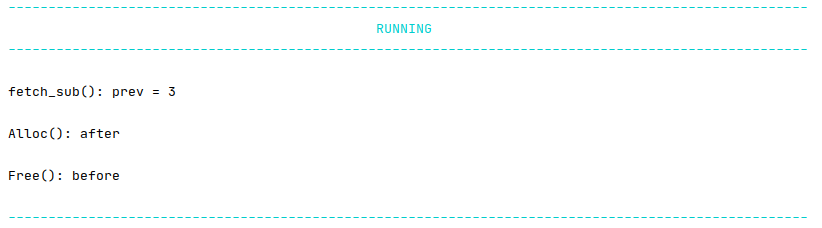
\includegraphics[scale=0.5]{running}}
	}
	\bigskip
	\caption{Заметки о событиях.}
\end{figure}

\end{itemize}

\section{Инженерные препятствия}

Model checker проверяет код, оптимизируемый компилятором. Поэтому нужно решать ряд трудностей, связанных непосредственно с языком программирования / оптимизациями компилятора.

\subsection{Абсолютные адреса и симметрия}

Для учета симметрии model checker канонизирует стеки, но этому процессу мешают абсолютные адреса:

\begin{itemize}
\item	При вызове функции на стек сохраняется указатель на начало родительского фрейма (значение регистра \mintinline{c++}{rbp}).

\item	На стеке может лежать ссылка на переменную, аллоцированную на этом стеке (в виде другой переменной или в виде значения регистра).

\item	В вызове \mintinline{c++}{Fork} перед переключением на контекст model checker-а вызывается служебная функция \mintinline{c++}{GetCurrentFiber}. В результате на стеке может “отпечататься” адрес текущего файбера.

\item	Файбер хранит исполняемую лямбду в type-erased контейнере. Для механизма type erasure требуется аллокация на куче. Так как такая аллокация происходит независимо для каждого файбера, все контейнеры получат свой собственный уникальный адрес в памяти, даже если отвечают одной лямбде. 
\end{itemize}

Канонизация очищает стек от внутренней адресации, адреса текущего файбера и адреса контейнера для исполняемой пользовательской функции.

Это только эвристика: model checker не может отличить адрес от числа, попавшего в тот же диапазон. Но на практике такие числа редко используются программой, и model checker находит баги.

\subsection{Встраивание вызовов}

Еще одна проблема – учет одинаковых состояний в бесконечных циклах. Бесконечные циклы возникают естественным образом: например, в тесте мьютекса поток в таком цикле захватывает и отпускает мьютекс.

Ожидается, что на каждой итерации стек файбера будет отличаться только состоянием локальных переменных, объявленных перед циклом. Поэтому граф состояний исполнения должен быть небольшим. 

Рассмотрим проблему на вышеупомянутом примере (захват и освобождение мьютекса в бесконечном цикле). Компилятор может встроить вызов \mintinline{c++}{lock} в итерацию цикла. Тогда инструкции \mintinline{c++}{lock}-а “засорят” регистры в фрейме цикла. В начале следующей итерации, когда вызовется \mintinline{c++}{Fork}, “мусорные” значения callee-saved регистров сохранятся на стеке – model checker сделает снимок формально другого состояния.

Но по сути поток вернулся к тому же состоянию, с которого начинал. Если бы вызов не встроился в цикл, то метод \mintinline{c++}{lock} на выходе восстановил бы значения тех callee-saved регистров, которыми пользовался. Значит, на следующей итерации при вызове \mintinline{c++}{Fork} на стек сохранились бы те же значения регистров, что и на предыдущей. Новое состояние бы не создалось.

Есть два решения проблемы:

\begin{itemize}
\item	Вместо цикла указать в конце итерации \mintinline{c++}{RestartFiber()} – служебную функцию model checker-а, которая полностью очищает стек и перезапускает исполняемую файбером функцию. Подходит только если между итерациями на стеке не сохраняется промежуточных переменных. 

\item	Запретить компилятору “засорять” фрейм цикла: поставить вызываемым из цикла методам атрибут \mintinline{c++}{noinline}.
\end{itemize}

\subsection{Выравнивание стека}

По ABI стек должен быть выровнен перед исполнением инструкции \mintinline{asm}{call}. Чтобы это сделать, компилятору выгоднее не двигать \mintinline{c++}{rsp} напрямую, а подвинуть \mintinline{c++}{rsp} с помощью \mintinline{asm}{push %rax} \autocite{Align}. Такой \mintinline{asm}{push} совершается с регистром, в котором хранится возвращаемое значение. Поэтому, даже если цикл использует только \mintinline{c++}{noinline}-функции, вызовы таких функций могли оставить на стеке следы результата предыдущей итерации. 

Решение – заставить компилятор выравнивать стек консервативно через атрибут \mintinline{c++}{force_align_arg_pointer}. Он служит для других целей, но подошел и для нашей – компилятор для функций с таким атрибутом будет изменять \mintinline{c++}{rsp} напрямую.


\chapter{Тестирование}\label{ch:ch3}

Реализованный model checker способен искать настоящие, нетривиальные ошибки в конкурентном коде. В этой главе мы продемонстрируем это утверждение на двух примерах: 

\section{LFAlloc}

Первый пример – это lock-free стек, выполняющий роль глобального кеша блоков в аллокаторе LFAlloc, который используется в алгоритме машинного обучения CatBoost и внутренних системах Яндекса \autocite{YaAlloc}. Реализация стека в ранней версии аллокатора содержала сложный сценарий ABA из нескольких десятков шагов. Уже после обнаружения ошибки для стека написали спецификацию на +Cal \autocite{YaSpec}, с помощью которой подтвердили наличие ошибки и верифицировали патч для нее.

Наш model checker находит тот же баг, но работает непосредственно с реализацией конкурентной структуры данных, а значит, не надо специфицировать стек на псевдокоде, расставлять метки атомарности, моделировать память и указатели.

%\iftoggleverb{pics}

\begin{figure}
	\centerfloat{
		\begin{tabular}{p{0.5\textwidth} p{0.5\textwidth}}
			\centering
			\vspace{0pt} \fbox{\parbox[t][.28\textheight]{0.48\textwidth}{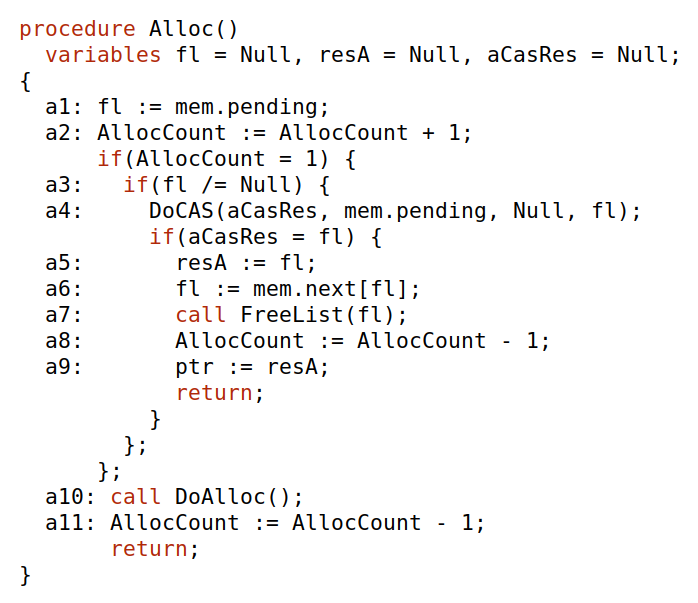
\includegraphics[width=0.48\textwidth]{specalloc}}}
			&
			\vspace{0pt} \fbox{\parbox[t][.28\textheight]{0.48\textwidth}{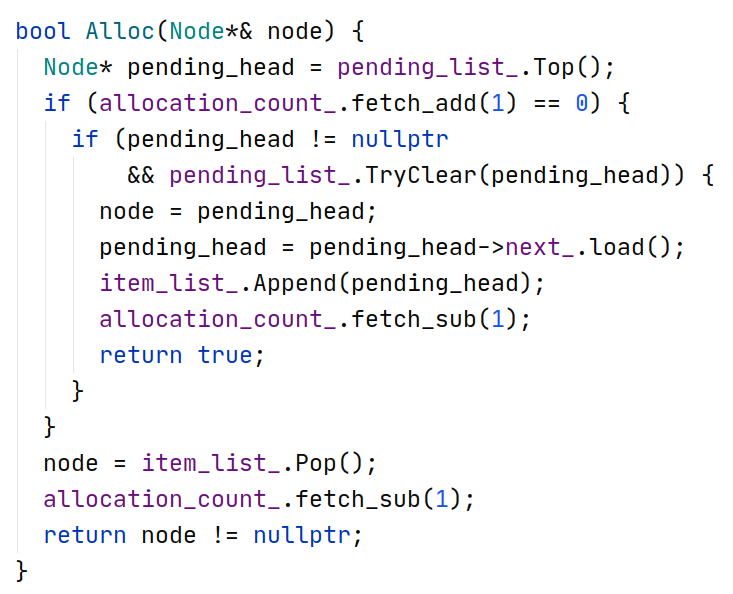
\includegraphics[width=0.48\textwidth]{checkeralloc}}}
			\\
			\hfil +Cal & \hfil \CC
		\end{tabular}
	}
	\bigskip
	\caption{Сравнение спецификации и кода на примере lock-free стека.}
\end{figure}

%\else
\begin{comment}

\begin{figure}
	\centerfloat{
		\begin{tabular}{p{0.5\textwidth} p{0.5\textwidth}}
			\centering
			
			\vspace{0pt}
			
			\fbox{\parbox[t][.28\textheight]{0.48\textwidth}{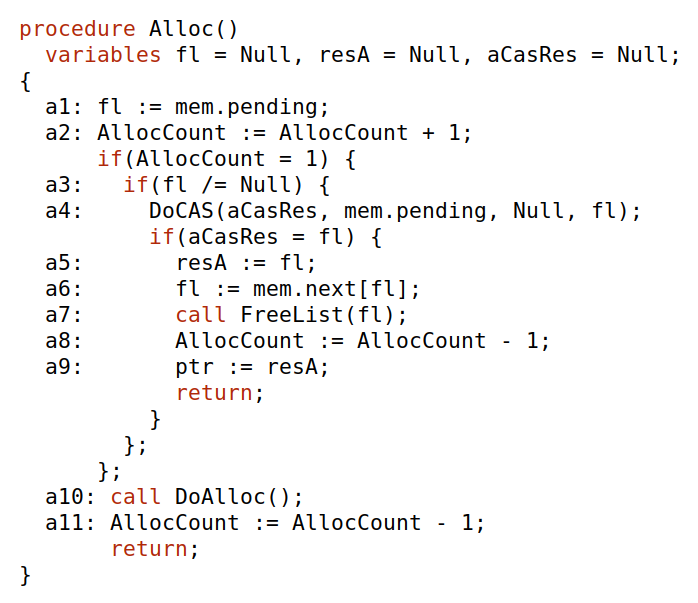
\includegraphics[width=0.48\textwidth]{specalloc}}}
			&
			\vspace{0pt} 
			
			\begin{minted}[fontsize=\tiny, frame=single, linenos=false]{c++}
 bool Alloc(Node*& node) {
	Node* pending_head = pending_list_.Top();
	if (allocation_count_.fetch_add(1) == 0) {
		if (pending_head != nullptr
		&& pending_list_.TryClear(pending_head)) {
			node = pending_head;
			pending_head = pending_head->next_.load();
			item_list_.Append(pending_head);
			allocation_count_.fetch_sub(1);
			return true;
		}
	}
	node = item_list_.Pop();
	allocation_count_.fetch_sub(1);
	return node != nullptr;
}
			\end{minted}
			
			
			\\
			\hfil +Cal & \hfil \CC
		\end{tabular}
	}
	\bigskip
	\caption{Сравнение спецификации и кода на примере lock-free стека.}
\end{figure}

%\fi
\end{comment}

При этом структуру теста можно не менять, а позаимствовать ее из спецификации на +Cal: поток в бесконечном цикле аллоцирует и деаллоцирует блоки памяти (узлы стека).

\begin{figure}
	\centerfloat{
		\begin{tabular}{p{0.5\textwidth} p{0.5\textwidth}}
			\centering
			\vspace{0pt} \fbox{\parbox[t][.2\textheight]{0.48\textwidth}{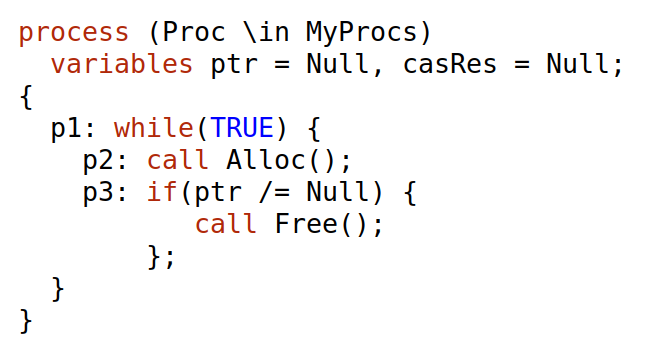
\includegraphics[width=0.48\textwidth]{spectest}}}
			&
			\vspace{0pt} \fbox{\parbox[t][.2\textheight]{0.48\textwidth}{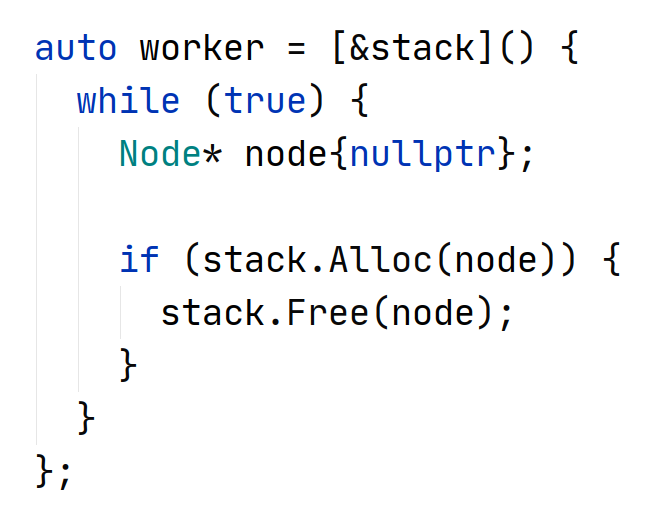
\includegraphics[width=0.38\textwidth]{checkertest}}}
			\\
			\hfil +Cal & \hfil \CC
		\end{tabular}
	}
	\bigskip
	\caption{Один и тот же тест для TLC и для model checker-а.}
\end{figure}

\begin{comment}

\begin{figure}
	\centerfloat{
		\begin{tabular}{p{0.5\textwidth} p{0.5\textwidth}}
			\centering
			\vspace{0pt} 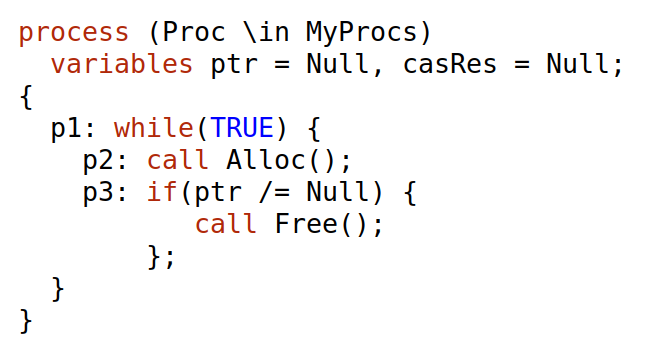
\includegraphics[width=0.5\textwidth]{spectest}
			&
			\vspace{0pt} 
			
			\begin{minted}{c++}
auto worker = [&stack]() {
	while (true) {
		Node* node{nullptr};

		if (stack.Alloc(node)) {
			stack.Free(node);
		}
	}
};
			\end{minted}
			
			\\
			\hfil +Cal & \hfil \CC
		\end{tabular}
	}
	\bigskip
	\caption{Один и тот же тест для TLC и для model checker-а.}
\end{figure}

\end{comment}

Реализация lock-free стека и тест для model checker-а приведены в приложении \ref{app:A}.

Траектория, напечатанная нашим model checker-ом (см. \ref{app:trace}), более читаема, чем траектория, которую печатает TLC: в ней для каждого шага печатается настоящий стектрейс и значения локальных переменных. По ней гораздо проще восстановить сценарий ABA.

Приведем статистику поиска данного бага model checker-ом и TLC:

%\begin{center}
\begin{table}
\centering
\begin{tabular}{| l | c | c |}
\hline
                   & model checker & TLC \\
                   \hline
 Длина траектории & 61 шаг & 76 шагов \\ 
 Найдено состояний & \numprint{17906188} & \numprint{26168885} \\  
 Найдено уникальных состояний & \numprint{4751588} & \numprint{7269203} \\
 Время                       & 29 cекунд & 8 минут\\
 	\hline
\end{tabular}

\bigskip
\captionsetup{justification=centering}
\caption{Статистика поиска ABA в LFAlloc.} 
\end{table}
%\end{center}

В четвертой главе будет описан инструмент model checker-а (недетерминизм, выражаемый в коде), который позволит сделать тест для стека более гибким – и, как следствие, сократить перебор и получить более короткую траекторию.

LFAlloc - пример со сложным (длинным) сценарием ABA. Следующий пример - про сложность другого рода: про поиск ошибки в большом коде.

\section{Executors}

Executors – фреймворк для асинхронного исполнения задач. Пользователю предоставляется сущность \emph{экзекьютора} (представленная интерфейсом \mintinline{c++}{IExecutor}) с единственной операцией – запланировать \emph{задачу} (произвольную функцию без аргументов и возвращаемого значения) для исполнения в некотором потоке.

Базовый экзекьютор – пул потоков фиксированного размера, разбирающих разделяемую очередь задач. Поверх этого пула можно писать декораторы, например, для последовательного исполнения задач или для поддержки приоритетов задач.

Код в таком фреймворке не похож на изолированную структуру данных: он гораздо больше и в нем много нетривильных конкурентных “деталей”: блокирующие и лок-фри очереди, спинлоки, вспомогательные примитивы синхронизации и т.п.

\iftoggleverb{pics}

\begin{figure}
	\centerfloat{
		\fbox{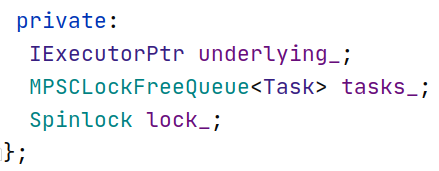
\includegraphics[scale=0.5]{strandfields}}
	}
	\bigskip
	\caption{Поля одного из экзекьюторов (Strand-а) – композиция конкурентных объектов.}\label{fig:strandfields}
\end{figure}

\else

\begin{listing}
	\centering
	
	\begin{minted}{c++}
    
class Strand : public IExecutor {
// implementation...

private:
	IExecutorPtr executor_;
	MPSCLockFreeQueue<Task> tasks_;
	Spinlock lock_;
};

	\end{minted}
	\caption{Поля одного из экзекьюторов (Strand-а) – композиция конкурентных объектов.}
	\label{strandfields}
\end{listing}

\fi

Рассмотрим \emph{Strand} (или \emph{Serial Executor}) – декоратор над пулом потоков, который исполняет все запланированные через него задачи в потоках декорируемого пула строго последовательно и в порядке их добавления.

В реализации этого декоратора легко допустить race condition при планировании / перепланировании служебной задачи, которая запускает пользовательские в потоках нижележащего пула. Такой race condition приведет к тому, что последняя пачка задач Strand-а может не выполниться.

\begin{figure}
	\centerfloat{
		\begin{tabular}{p{0.5\textwidth}p{0.5\textwidth}}
			\centering
			\vspace{0pt} \fbox{\parbox[t][.29\textheight]{0.48\textwidth}{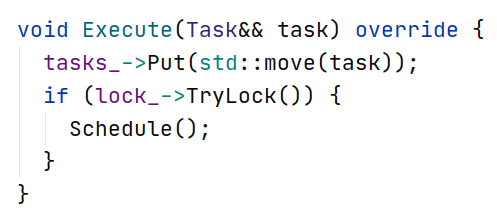
\includegraphics[width=0.48\textwidth]{exec}}}
			&
			\vspace{0pt} \fbox{\parbox[t][.29\textheight]{0.48\textwidth}{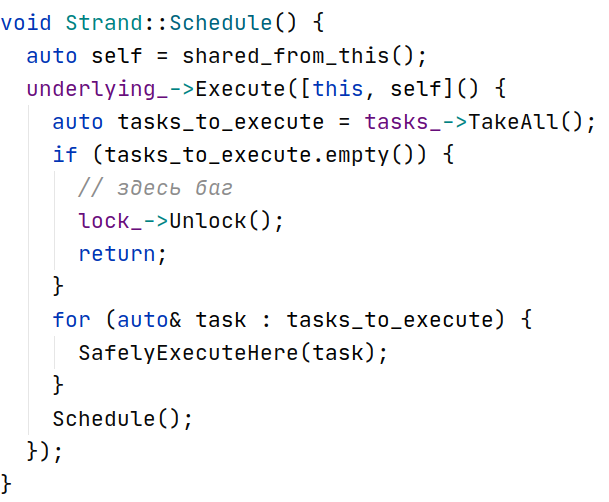
\includegraphics[width=0.48\textwidth]{sched}}}
		\end{tabular}
	}
	\bigskip
	\caption{Фрагменты неправильной реализации Strand-а.}
\end{figure}

Тест на такую ошибку в model checker-е устроен просто: в Strand последовательно добавляются две задачи, пул останавливается, после чего проверяется счетчик выполненных задач:

\iftoggleverb{pics}

\begin{figure}
	\centerfloat{
		\fbox{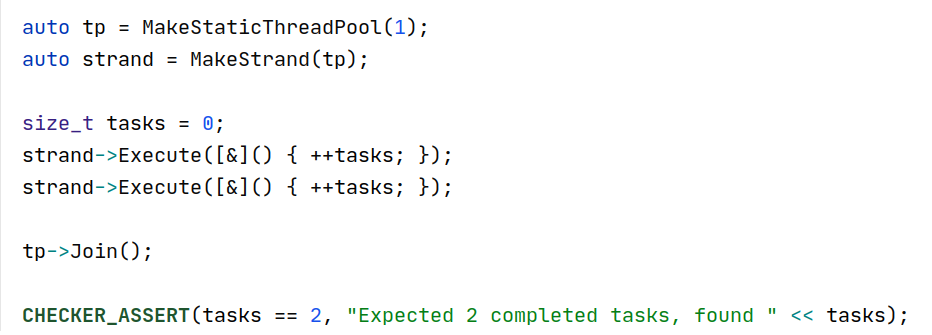
\includegraphics[scale=0.5]{strandtest}}
	}
	\bigskip
	\caption{Тест для Strand-а.}\label{fig:strandtest}
\end{figure}

\else

\begin{listing}
	\centering
	
	\begin{minted}{c++}
    
auto tp = MakeStaticThreadPool(1);
auto strand = MakeStrand(tp);

size_t tasks = 0;
strand->Execute([&]() { ++tasks; });
strand->Execute([&]() { ++tasks; });

tp->Join();

CHECKER_ASSERT(tasks == 2, "Expected 2 completed tasks, found " << tasks);

	\end{minted}
	\caption{Тест Strand-а.}
	\label{strandtest}
\end{listing}

\fi

Несмотря на простоту теста, за счет перебора всех исполнений model checker находит описанный выше race condition.

\chapter{Инструменты пользователя}\label{ch:ch4}

В этой главе мы опишем инструменты, с помощью которых пользователь может настраивать поведение model checker-а.

\section{Атомарность}

Если верифицируемый код устроен достаточно сложно (использует сразу несколько конкурентных примитивов / структур данных), то найденная model checker-ом траектория получится длинной и потому плохо читаемой – в ней будет слишком много действий, не относящихся непосредственно к найденному race condition-у.

Например, Strand / Serial Executor использует lock-free очередь, которая генерирует в траектории много промежуточных состояний, но ошибка в Strand-е, на которой в предыдущей главе проверялся model checker, кроется не в очереди.

Другая ситуация: мы уверены в корректности той же lock-free очереди (пусть мы верифицировали ее независимо) и хотим сократить перебор в model checker-е.

В описанных ситуациях удобно предположить, что lock-free очередь линеаризуема (атомарна) и не ветвить исполнение внутри реализации ее методов.

Аннотировать линеаризуемый объект можно с помощью декоратора \mintinline{c++}{ForkGuarded<T>}, который проксирует все вызовы методов объекта:

\begin{enumerate}
\item	Вызывает \mintinline{c++}{Fork} (вызов метода – ровно одна развилка).

\item	Выключает \mintinline{c++}{Fork} на время жизни проксирующего вызов объекта.

\item	Вызывает метод объекта, внутри которого ветвлений уже не будет.
\end{enumerate}

По сути, декоратор \mintinline{c++}{ForkGuarded<T>} – это прямой аналог метки в +Cal, он позволяет регулировать гранулярность атомарности для model checker-а. Но, в отличие от меток, этот механизм более безопасный: атомарность устанавливается на объекте, а не на отдельных фрагментах кода.

\iftoggleverb{pics}

\begin{figure}
	\centerfloat{
		\fbox{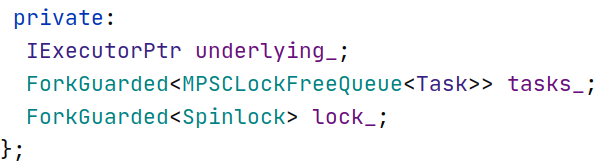
\includegraphics[scale=0.5]{forkguarded}}
	}
	\bigskip
	\caption{\mintinline{c++}{ForkGuarded<T>} в Strand-е.}
\end{figure}

\else

\begin{listing}
	\centering
	
	\begin{minted}{c++}
class Strand : public IExecutor {
// implementation...

private:
	IExecutorPtr executor_;
	ForkGuarded<MPSCLockFreeQueue<Task>> tasks_;
	ForkGuarded<Spinlock> lock_;
};
	\end{minted}
	\caption{\mintinline{c++}{ForkGuarded<T>} в Strand-е.}
	
\end{listing}

\fi


\section{Either / Random}

Чтобы перебрать больше сценариев в тесте, разветвлять можно и сам код. 

Для примера возьмем спинлок с методами \mintinline{c++}{Lock} и \mintinline{c++}{TryLock}. Естественный тест для него – это захват и освобождение лока в бесконечном цикле. У потока есть два варианта, как взять лок, и хочется проверить оба. В +Cal для этого есть конструкция \mintinline{c++}{either} / \mintinline{c++}{or}: она создает развилку в коде, в которой model checker пройдет по обеим веткам исполнения:

\begin{figure}
	\centerfloat{
		\fbox{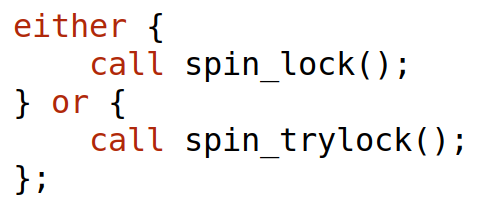
\includegraphics[scale=0.4]{caleither}}
	}
	\bigskip
	\caption{\mintinline{c++}{either} из +Cal.}
\end{figure}


В model checker-е для аналогичных целей реализована функция \mintinline{text}{bool Either()}. Вызов функции переключается на контекст model checker-а, и тот кладет в очередь состояний не один снимок, а два – каждый со своим выходом из \mintinline{c++}{Either}. Чтобы не создавать два почти одинаковых снимка состояния, model checker продолжает оба состояния еще на один шаг вперед. 

\iftoggleverb{pics}

%\begin{comment}
\begin{figure}
	\centerfloat{
		\fbox{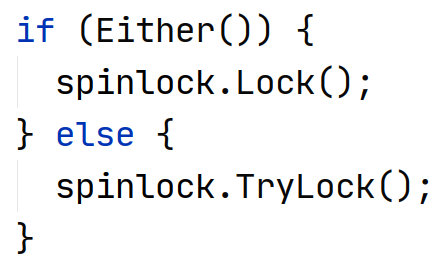
\includegraphics[scale=0.35]{either}}
	}
	\bigskip
	\caption{\mintinline{text}{Either} model checker-а.}
\end{figure}
%\end{comment}

\else

\begin{listing}
	\centering
	
	\begin{minted}{c++}
if (Either()) {
	lock.Lock();
} else {
	lock.TryLock();
}
	\end{minted}
	\caption{Тест для спинлока с Either.}
	
\end{listing}

\fi

Можно создавать не две, а произвольное число новых веток. Такая логика реализуется функцией \mintinline{text}{size_t Random(size_t n)}: она порождает $n$ новых продолжений, каждое с уникальным возвращаемым значением от $0$ до $n-1$. 

\mintinline{c++}{Random} позволяет писать тесты с более разнообразными сценариями исполнения. В +Cal-версии теста для LFAlloc поток всегда сначала аллоцирует узел, а потом возвращает обратно. Вместо этого поток может узнать, сколько узлов уже аллоцировано ($n$), и сгенерировать “случайное” значение с помощью \mintinline{c++}{Random(n+1)}. Если сгенерированное значение – $0$, поток аллоцирует еще один узел (вынимает из стека). Иначе – вызывает \mintinline{c++}{Free} на узле с полученным “случайным” индексом (возвращает в стек). Так потоки не будут привязаны к последовательности действий “\mintinline{c++}{Alloc} – \mintinline{c++}{Free} – \mintinline{c++}{Alloc} – \mintinline{c++}{Free} … “. Новому сценарию достаточно трех потоков вместо четырех для нарушения инварианта, время теста сокращается в шесть раз, а траектория получается короче – она не содержит лишних действий, появившихся из-за фиксированной структуры теста.

\iftoggleverb{pics}

\begin{figure}
	\centerfloat{
		\fbox{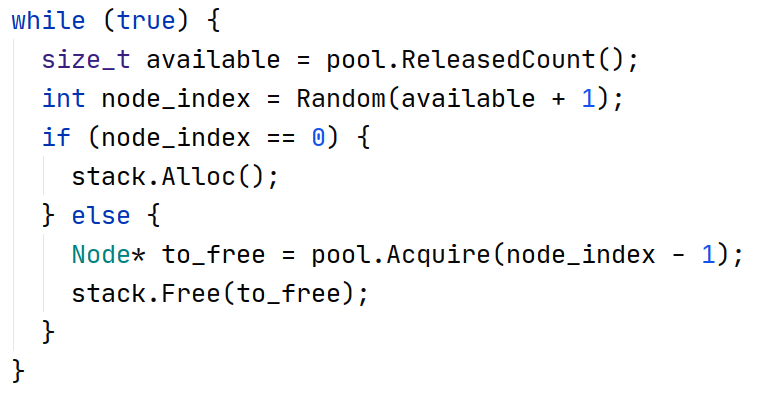
\includegraphics[scale=0.4]{stackrandom}}
	}
	\bigskip
	\caption{\mintinline{c++}{Random} в тесте lock-free стека.}
\end{figure}


\else

\begin{listing}
	\centering
	
	\begin{minted}{c++}
while (true) {
	size_t available = pool.ReleasedCount();
	int node_index = Random(available + 1);
	if (node_index == 0) {
		stack.Alloc();
	} else {
		Node* to_free = pool.Acquire(node_index - 1);
		stack.Free(to_free);
	}
}
	\end{minted}
	\caption{Random в тесте lock-free стека.}
	
\end{listing}

\fi 

Приведем окончательную статистику тестирования lock-free стека в LFAlloc:

\begin{table}
\centering
\begin{tabular}{| l | >{\bfseries}c | c | c |}
\hline
                              & \makecell{model checker \\ (с \mintinline{c++}{Random})}         & \makecell{model checker \\ (без \mintinline{c++}{Random})}  & TLC \\
                   \hline    
 Длина траектории             & 50 шагов                         & 61 шаг                      & 76 шагов \\ 
 Найдено состояний            & \numprint{2574023}               & \numprint{17906188}         & \numprint{26168885} \\      
 \makecell[l]{Найдено уникальных \\ состояний} & \numprint{789596}                & \numprint{4751588}          & \numprint{7269203} \\
 Время                        & 5 секунд                         & 29 cекунд                   & 8 минут\\
 	\hline
\end{tabular}

\bigskip
\captionsetup{justification=centering}
\caption{Статистика (с \mintinline{c++}{Random} и без) поиска ABA в LFAlloc.} 
\end{table}

Кроме того, функцию \mintinline{c++}{Random} использует сам model checker в реализации очереди ожидания в мьютексах и условных переменных: с помощью \mintinline{c++}{Random(n)} в \mintinline{c++}{WakeOne} он  может “недетерминированно” разбудить любой из $n$ спящих в очереди потоков.

\iftoggleverb{pics}

%\begin{comment}
	\begin{figure}
	\centerfloat{
		\fbox{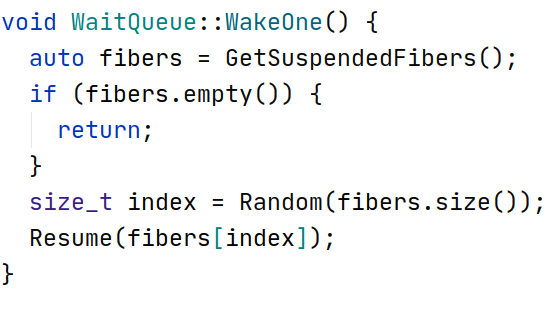
\includegraphics[scale=0.5]{wakeone}}
	}
	\bigskip
	\caption{\mintinline{c++}{Random} в реализации очереди ожидания.}
\end{figure}
%\end{comment}

\else

\begin{listing}
\centering

\begin{minted}{c++}
void WaitQueue::WakeOne() {
	auto fibers = GetSuspendedFibers();
	if (fibers.empty()) {
		return;
	}
	size_t index = Random(fibers.size());
	Resume(fibers[index]);
}
\end{minted}
\caption{Random в реализации очереди ожидания.}

\end{listing}

\fi


\section{Prune}

Служебная функция \mintinline{c++}{Prune} выбрасывает из рассмотрения текущее состояние.

\mintinline{c++}{Prune} можно использовать для проверки тестов с бесконечным графом исполнения. Например, мы хотим написать тест для ticket lock-а – но атомарный счетчик свободных билетов растет в нем бесконечно. Чтобы ограничить граф состояний, вызовем \mintinline{c++}{Prune} в местах, где билет становится больше какого-то порога: 

\iftoggleverb{pics}

\begin{figure}
	\centerfloat{
		\fbox{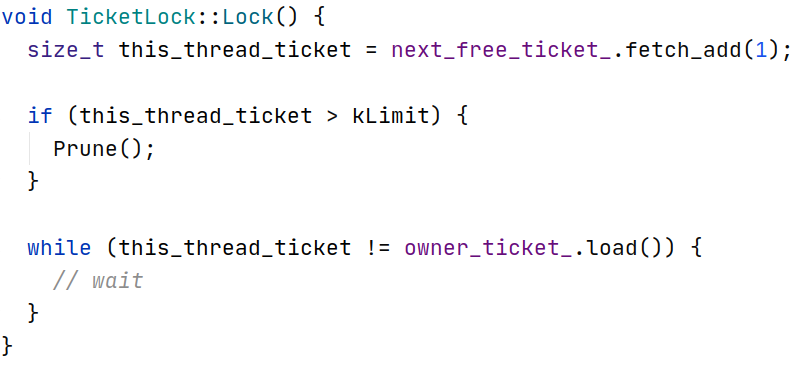
\includegraphics[scale=0.5]{prune}}
	}
	\bigskip
	\caption{\mintinline{c++}{Prune} в ticket lock.}
\end{figure}

\else

\begin{listing}
	\centering
	
	\begin{minted}{c++}
void TicketLock::Lock() {
	size_t this_thread_ticket = next_free_ticket_.fetch_add(1);

	if (this_thread_ticket > kLimit) {
		Prune();
	}

	while (this_thread_ticket != owner_ticket_.load()) {
		// wait
	}
}
	\end{minted}
	\caption{Prune в ticket lock.}
	
\end{listing}

\fi

Еще одно потенциальное применение \mintinline{c++}{Prune} – отсечение неперспективных веток исполнения для ускорения перебора.

\section{Детализация траектории}


\subsection{Заметки о событиях}

Подобно логированию, траекторию model checker-а можно детализировать заметками с помощью макроса \mintinline{c++}{SHOW_NOTE(message)}.

Заметки делятся на два типа:

\begin{itemize}
\item	Служебные – заметки, уже встроенные в атомики / примитивы синхронизации: результат чтения атомика, парковка потока на условной переменной, состояние очереди ожидания мьютекса. 

\begin{figure}
	\centerfloat{
		\fbox{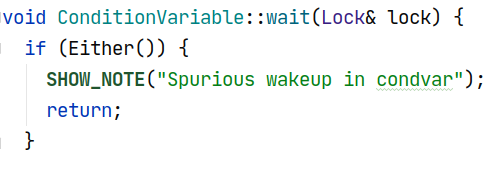
\includegraphics[scale=0.5]{spurcond}}
	}
	\bigskip
	\caption{Служебная заметка.}
\end{figure}

\item	Пользовательские – “отладочные” комментарии: поток зашел в определенную ветку кода, завершил какую-то операцию и т.п.

\begin{figure}
	\centerfloat{
		\fbox{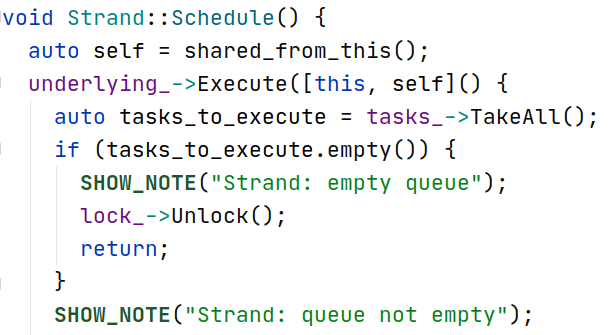
\includegraphics[scale=0.45]{shownote}}
	}
	\bigskip
	\caption{Пользовательские заметки.}
\end{figure}

\end{itemize}

\subsection{Описание разделяемого состояния}

При печати траектории model checker автоматически показывает стеки вызовов и состояние локальных переменных. Но об устройстве глобального состояния он ничего не знает.

Чтобы каждый “шаг” траектории сопровождался представлением разделяемого состояния, пользователь должен в начале теста передать функцию печати model checker-у с помощью вызова \mintinline{c++}{PrintState(std::function<StateDescription()>)}.

Описание задается в виде \mintinline{c++}{StateDescription} – объекта, который model checker уже умеет печатать (в json-подобном виде). \mintinline{c++}{StateDescription} строится инкрементально двумя способами:

\begin{itemize}
\item	передачей пары “ключ – значение”;

\item	передачей вложенного \mintinline{c++}{StateDescription}-а.
\end{itemize}

\iftoggleverb{pics}

\begin{figure}
	\centerfloat{
		\fbox{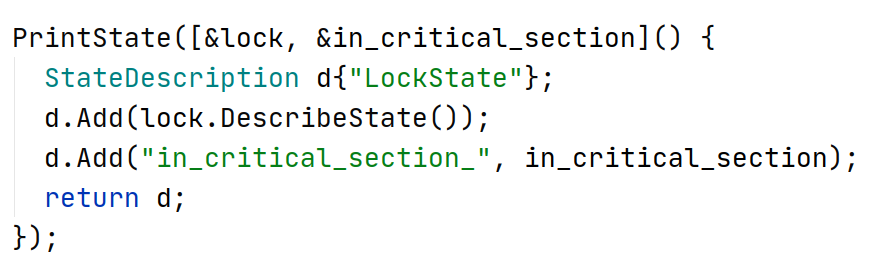
\includegraphics[scale=0.35]{descr}}
	}
	\bigskip
	\caption{Описание разделяемого состояния в тесте спинлока.}\label{fig:descr}
\end{figure}

\else

\begin{listing}
	\centering
	
	\begin{minted}{c++}
PrintState([&lock, &in_critical_section]() {
	StateDescription d{"LockState"};
	d.Add(lock.DescribeState());
	d.Add("in_critical_section_", in_critical_section);
	return d;
});
	\end{minted}
	\caption{Описание разделяемого состояния.}
	
\end{listing}

\fi

\chapter{Заключение}



\section{Результаты}

Реализован model checker, который для многопоточного теста на C++ проверяет заданный инвариант во всех возможных состояниях, достижимых при исполнении этого теста. При нарушении инварианта model checker печатает кратчайшую детализированную траекторию, которая приводит к этому.

Model checker протестирован на нетривиальных примерах: он находит сложные баги из десятков шагов (ABA в lock-free стеке) и способен проверять сложный составной код (фреймворк экзекьюторов). 

Реализованы и описаны инструменты  для управления перебором в model checker-е: \mintinline{c++}{ForkGuarded<T>} для управления гранулярностью атомарности, \mintinline{c++}{Either} / \mintinline{c++}{Random} для выражения недетерминированного ветвления, \mintinline{c++}{Prune} для отсечения перебора. 

\section{Направления для дальнейшего исследования}

\begin{itemize}

\item	Поддержать слабые модели памяти.

\item	Автоматически инструментировать тестируемый код.

\end{itemize}



%\include{Dissertation/introduction}    % Введение
%\ifnumequal{\value{contnumfig}}{1}{\counterwithout{figure}{chapter}
%}{\counterwithin{figure}{chapter}}
%\ifnumequal{\value{contnumtab}}{1}{\counterwithout{table}{chapter}
%}{\counterwithin{table}{chapter}}
%\chapter{Оформление различных элементов}\label{ch:ch10}

\section{Форматирование текста}\label{sec:ch10/sec1}

Мы можем сделать \textbf{жирный текст} и \textit{курсив}.

\section{Ссылки}\label{sec:ch10/sec2}

Сошлёмся на библиографию.
Одна ссылка: \cite[с.~54]{Sokolov}\cite[с.~36]{Gaidaenko}.
Две ссылки: \cite{Sokolov,Gaidaenko}.
Ссылка на собственные работы: \cite{vakbib1, confbib2}.
Много ссылок: %\cite[с.~54]{Lermontov,Management,Borozda} % такой «фокус»
%вызывает biblatex warning относительно опции sortcites, потому что неясно, к
%какому источнику относится уточнение о страницах, а bibtex об этой проблеме
%даже не предупреждает
\cite{Lermontov, Management, Borozda, Marketing, Constitution, FamilyCode,
Gost.7.0.53, Razumovski, Lagkueva, Pokrovski, Methodology, Nasirova, Berestova,
Kriger}%
\ifnumequal{\value{bibliosel}}{0}{% Примеры для bibtex8
    \cite{Sirotko, Lukina, Encyclopedia}%
}{% Примеры для biblatex через движок biber
    \cite{Sirotko2, Lukina2, Encyclopedia2}%
}%
.
И~ещё немного ссылок:~\cite{Article,Book,Booklet,Conference,Inbook,Incollection,Manual,Mastersthesis,
Misc,Phdthesis,Proceedings,Techreport,Unpublished}
% Следует обратить внимание, что пробел после запятой внутри \cite{}
% обрабатывается ожидаемо, а пробел перед запятой, может вызывать проблемы при
% обработке ссылок.
\cite{medvedev2006jelektronnye, CEAT:CEAT581, doi:10.1080/01932691.2010.513279,
Gosele1999161,Li2007StressAnalysis, Shoji199895, test:eisner-sample,
test:eisner-sample-shorted, AB_patent_Pomerantz_1968, iofis_patent1960}
\ifnumequal{\value{bibliosel}}{0}{% Примеры для bibtex8
}{% Примеры для biblatex через движок biber
    \cite{patent2h, patent3h, patent2}%
}%
.

\ifnumequal{\value{bibliosel}}{0}{% Примеры для bibtex8
Попытка реализовать несколько ссылок на конкретные страницы
для \texttt{bibtex} реализации библиографии:
[\citenum{Sokolov}, с.~54; \citenum{Gaidaenko}, с.~36].
}{% Примеры для biblatex через движок biber
Несколько источников (мультицитата):
% Тут специально написано по-разному тире, для демонстрации, что
% применение специальных тире в настоящий момент в biblatex приводит к непоказу
% "с.".
\cites[vii--x, 5, 7]{Sokolov}[v"--~x, 25, 526]{Gaidaenko}[vii--x, 5, 7]{Techreport},
работает только в \texttt{biblatex} реализации библиографии.
}%

Ссылки на собственные работы:~\cite{vakbib1, confbib1}

Сошлёмся на приложения: Приложение~\ref{app:A}, Приложение~\ref{app:B2}.

Сошлёмся на формулу: формула~\eqref{eq:equation1}.

Сошлёмся на изображение: рисунок~\ref{fig:knuth}.

Стандартной практикой является добавление к ссылкам префикса, характеризующего тип элемента.
Это не является строгим требованием, но~позволяет лучше ориентироваться в документах большого размера.
Например, для ссылок на~рисунки используется префикс \textit{fig},
для ссылки на~таблицу "--- \textit{tab}.

В таблице~\ref{tab:tab_pref} приложения~\ref{app:B4} приведён список рекомендуемых
к использованию стандартных префиксов.

\section{Формулы}\label{sec:ch10/sec3}

Благодаря пакету \textit{icomma}, \LaTeX~одинаково хорошо воспринимает
в~качестве десятичного разделителя и запятую (\(3,1415\)), и точку (\(3.1415\)).

\subsection{Ненумерованные одиночные формулы}\label{subsec:ch10/sec3/sub1}

Вот так может выглядеть формула, которую необходимо вставить в~строку
по~тексту: \(x \approx \sin x\) при \(x \to 0\).

А вот так выглядит ненумерованная отдельностоящая формула c подстрочными
и надстрочными индексами:
\[
(x_1+x_2)^2 = x_1^2 + 2 x_1 x_2 + x_2^2
\]

Формула с неопределенным интегралом:
\[
\int f(\alpha+x)=\sum\beta
\]

При использовании дробей формулы могут получаться очень высокие:
\[
  \frac{1}{\sqrt{2}+
  \displaystyle\frac{1}{\sqrt{2}+
  \displaystyle\frac{1}{\sqrt{2}+\cdots}}}
\]

В формулах можно использовать греческие буквы:
%Все \original... команды заранее, ради этого примера, определены в Dissertation\userstyles.tex
\[
\alpha\beta\gamma\delta\originalepsilon\epsilon\zeta\eta\theta%
\vartheta\iota\kappa\varkappa\lambda\mu\nu\xi\pi\varpi\rho\varrho%
\sigma\varsigma\tau\upsilon\originalphi\phi\chi\psi\omega\Gamma\Delta%
\Theta\Lambda\Xi\Pi\Sigma\Upsilon\Phi\Psi\Omega
\]
\[%https://texfaq.org/FAQ-boldgreek
\boldsymbol{\alpha\beta\gamma\delta\originalepsilon\epsilon\zeta\eta%
\theta\vartheta\iota\kappa\varkappa\lambda\mu\nu\xi\pi\varpi\rho%
\varrho\sigma\varsigma\tau\upsilon\originalphi\phi\chi\psi\omega\Gamma%
\Delta\Theta\Lambda\Xi\Pi\Sigma\Upsilon\Phi\Psi\Omega}
\]

Для добавления формул можно использовать пары \verb+$+\dots\verb+$+ и \verb+$$+\dots\verb+$$+,
но~они считаются устаревшими.
Лучше использовать их функциональные аналоги \verb+\(+\dots\verb+\)+ и \verb+\[+\dots\verb+\]+.

\subsection{Ненумерованные многострочные формулы}\label{subsec:ch10/sec3/sub2}

Вот так можно написать две формулы, не нумеруя их, чтобы знаки <<равно>> были
строго друг под другом:
\begin{align}
  f_W & =  \min \left( 1, \max \left( 0, \frac{W_{soil} / W_{max}}{W_{crit}} \right)  \right), \nonumber \\
  f_T & =  \min \left( 1, \max \left( 0, \frac{T_s / T_{melt}}{T_{crit}} \right)  \right), \nonumber
\end{align}

Выровнять систему ещё и по переменной \( x \) можно, используя окружение
\verb|alignedat| из пакета \verb|amsmath|. Вот так:
\[
    |x| = \left\{
    \begin{alignedat}{2}
        &&x, \quad &\text{eсли } x\geqslant 0 \\
        &-&x, \quad & \text{eсли } x<0
    \end{alignedat}
    \right.
\]
Здесь первый амперсанд (в исходном \LaTeX\ описании формулы) означает
выравнивание по~левому краю, второй "--- по~\( x \), а~третий "--- по~слову
<<если>>. Команда \verb|\quad| делает большой горизонтальный пробел.

Ещё вариант:
\[
    |x|=
    \begin{cases}
    \phantom{-}x, \text{если } x \geqslant 0 \\
    -x, \text{если } x<0
    \end{cases}
\]

Кроме того, для  нумерованных формул \verb|alignedat| делает вертикальное
выравнивание номера формулы по центру формулы. Например, выравнивание
компонент вектора:
\begin{equation}
\label{eq:2p3}
\begin{alignedat}{2}
{\mathbf{N}}_{o1n}^{(j)} = \,{\sin} \phi\,n\!\left(n+1\right)
         {\sin}\theta\,
         \pi_n\!\left({\cos} \theta\right)
         \frac{
               z_n^{(j)}\!\left( \rho \right)
              }{\rho}\,
           &{\boldsymbol{\hat{\mathrm e}}}_{r}\,+   \\
+\,
{\sin} \phi\,
         \tau_n\!\left({\cos} \theta\right)
         \frac{
            \left[\rho z_n^{(j)}\!\left( \rho \right)\right]^{\prime}
              }{\rho}\,
            &{\boldsymbol{\hat{\mathrm e}}}_{\theta}\,+   \\
+\,
{\cos} \phi\,
         \pi_n\!\left({\cos} \theta\right)
         \frac{
            \left[\rho z_n^{(j)}\!\left( \rho \right)\right]^{\prime}
              }{\rho}\,
            &{\boldsymbol{\hat{\mathrm e}}}_{\phi}\:.
\end{alignedat}
\end{equation}

Ещё об отступах. Иногда для лучшей <<читаемости>> формул полезно
немного исправить стандартные интервалы \LaTeX\ с учётом логической
структуры самой формулы. Например в формуле~\ref{eq:2p3} добавлен
небольшой отступ \verb+\,+ между основными сомножителями, ниже
результат применения всех вариантов отступа:
\begin{align*}
\backslash! &\quad f(x) = x^2\! +3x\! +2 \\
  \mbox{по-умолчанию} &\quad f(x) = x^2+3x+2 \\
\backslash, &\quad f(x) = x^2\, +3x\, +2 \\
\backslash{:} &\quad f(x) = x^2\: +3x\: +2 \\
\backslash; &\quad f(x) = x^2\; +3x\; +2 \\
\backslash \mbox{space} &\quad f(x) = x^2\ +3x\ +2 \\
\backslash \mbox{quad} &\quad f(x) = x^2\quad +3x\quad +2 \\
\backslash \mbox{qquad} &\quad f(x) = x^2\qquad +3x\qquad +2
\end{align*}

Можно использовать разные математические алфавиты:
\begin{align}
\mathcal{ABCDEFGHIJKLMNOPQRSTUVWXYZ} \nonumber \\
\mathfrak{ABCDEFGHIJKLMNOPQRSTUVWXYZ} \nonumber \\
\mathbb{ABCDEFGHIJKLMNOPQRSTUVWXYZ} \nonumber
\end{align}

Посмотрим на систему уравнений на примере аттрактора Лоренца:

\[
\left\{
  \begin{array}{rl}
    \dot x = & \sigma (y-x) \\
    \dot y = & x (r - z) - y \\
    \dot z = & xy - bz
  \end{array}
\right.
\]

А для вёрстки матриц удобно использовать многоточия:
\[
\left(
  \begin{array}{ccc}
    a_{11} & \ldots & a_{1n} \\
    \vdots & \ddots & \vdots \\
    a_{n1} & \ldots & a_{nn} \\
  \end{array}
\right)
\]

\subsection{Нумерованные формулы}\label{subsec:ch10/sec3/sub3}

А вот так пишется нумерованная формула:
\begin{equation}
  \label{eq:equation1}
  e = \lim_{n \to \infty} \left( 1+\frac{1}{n} \right) ^n
\end{equation}

Нумерованных формул может быть несколько:
\begin{equation}
  \label{eq:equation2}
  \lim_{n \to \infty} \sum_{k=1}^n \frac{1}{k^2} = \frac{\pi^2}{6}
\end{equation}

Впоследствии на формулы~\eqref{eq:equation1} и~\eqref{eq:equation2} можно ссылаться.

Сделать так, чтобы номер формулы стоял напротив средней строки, можно,
используя окружение \verb|multlined| (пакет \verb|mathtools|) вместо
\verb|multline| внутри окружения \verb|equation|. Вот так:
\begin{equation} % \tag{S} % tag - вписывает свой текст
  \label{eq:equation3}
    \begin{multlined}
        1+ 2+3+4+5+6+7+\dots + \\
        + 50+51+52+53+54+55+56+57 + \dots + \\
        + 96+97+98+99+100=5050
    \end{multlined}
\end{equation}

Используя команду \verb|\eqrefs|, можно
красиво ссылаться сразу на несколько формул
\eqrefs{eq:equation1, eq:equation3, eq:equation2}, даже перепутав
порядок ссылок \verb|\eqrefs{eq1, eq3, eq2}|.
Аналогично, для ссылок на несколько рисунков, таблиц и~т.\:д.
\refs{sec:ch10/sec1, sec:ch10/sec2, sec:ch10/sec3} можно использовать
команду \verb|\refs|.
Обе эти команды определены в файле \verb|common/packages.tex|.

Уравнения~\eqrefs{eq:subeq_1,eq:subeq_2} демонстрируют возможности
окружения \verb|\subequations|.
\begin{subequations}
    \label{eq:subeq_1}
    \begin{gather}
        y = x^2 + 1 \label{eq:subeq_1-1} \\
        y = 2 x^2 - x + 1 \label{eq:subeq_1-2}
    \end{gather}
\end{subequations}
Ссылки на отдельные уравнения~\eqrefs{eq:subeq_1-1,eq:subeq_1-2,eq:subeq_2-1}.
\begin{subequations}
    \label{eq:subeq_2}
    \begin{align}
        y &= x^3 + x^2 + x + 1 \label{eq:subeq_2-1} \\
        y &= x^2
    \end{align}
\end{subequations}

\subsection{Форматирование чисел и размерностей величин}\label{sec:units}

Числа форматируются при помощи команды \verb|\num|:
\num{5,3};
\num{2,3e8};
\num{12345,67890};
\num{2,6 d4};
\num{1+-2i};
\num{.3e45};
\num[exponent-base=2]{5 e64};
\num[exponent-base=2,exponent-to-prefix]{5 e64};
\num{1.654 x 2.34 x 3.430}
\num{1 2 x 3 / 4}.
Для написания последовательности чисел можно использовать команды \verb|\numlist| и \verb|\numrange|:
\numlist{10;30;50;70}; \numrange{10}{30}.
Значения углов можно форматировать при помощи команды \verb|\ang|:
\ang{2.67};
\ang{30,3};
\ang{-1;;};
\ang{;-2;};
\ang{;;-3};
\ang{300;10;1}.

Обратите внимание, что ГОСТ запрещает использование знака <<->> для обозначения отрицательных чисел
за исключением формул, таблиц и~рисунков.
Вместо него следует использовать слово <<минус>>.

Размерности можно записывать при помощи команд \verb|\si| и \verb|\SI|:
\si{\farad\squared\lumen\candela};
\si{\joule\per\mole\per\kelvin};
\si[per-mode = symbol-or-fraction]{\joule\per\mole\per\kelvin};
\si{\metre\per\second\squared};
\SI{0.10(5)}{\neper};
\SI{1.2-3i e5}{\joule\per\mole\per\kelvin};
\SIlist{1;2;3;4}{\tesla};
\SIrange{50}{100}{\volt}.
Список единиц измерений приведён в таблицах~\refs{tab:unit:base,
tab:unit:derived,tab:unit:accepted,tab:unit:physical,tab:unit:other}.
Приставки единиц приведены в~таблице~\ref{tab:unit:prefix}.

С дополнительными опциями форматирования можно ознакомиться в~описании пакета \texttt{siunitx};
изменить или добавить единицы измерений можно в~файле \texttt{siunitx.cfg}.

\begin{table}
    \centering
    \captionsetup{justification=centering} % выравнивание подписи по-центру
    \caption{Основные величины СИ}\label{tab:unit:base}
    \begin{tabular}{llc}
        \toprule
        Название  & Команда                & Символ         \\
        \midrule
        Ампер     & \verb|\ampere| & \si{\ampere}   \\
        Кандела   & \verb|\candela| & \si{\candela}  \\
        Кельвин   & \verb|\kelvin| & \si{\kelvin}   \\
        Килограмм & \verb|\kilogram| & \si{\kilogram} \\
        Метр      & \verb|\metre| & \si{\metre}    \\
        Моль      & \verb|\mole| & \si{\mole}     \\
        Секунда   & \verb|\second| & \si{\second}   \\
        \bottomrule
    \end{tabular}
\end{table}

\begin{table}
  \small
  \centering
  \begin{threeparttable}% выравнивание подписи по границам таблицы
    \caption{Производные единицы СИ}\label{tab:unit:derived}
    \begin{tabular}{llc|llc}
        \toprule
        Название       & Команда                 & Символ              & Название & Команда & Символ \\
        \midrule
        Беккерель      & \verb|\becquerel|  & \si{\becquerel}     &
        Ньютон         & \verb|\newton|  & \si{\newton}                                      \\
        Градус Цельсия & \verb|\degreeCelsius| & \si{\degreeCelsius} &
        Ом             & \verb|\ohm| & \si{\ohm}                                         \\
        Кулон          & \verb|\coulomb| & \si{\coulomb}       &
        Паскаль        & \verb|\pascal| & \si{\pascal}                                      \\
        Фарад          & \verb|\farad| & \si{\farad}         &
        Радиан         & \verb|\radian| & \si{\radian}                                      \\
        Грей           & \verb|\gray| & \si{\gray}          &
        Сименс         & \verb|\siemens| & \si{\siemens}                                     \\
        Герц           & \verb|\hertz| & \si{\hertz}         &
        Зиверт         & \verb|\sievert| & \si{\sievert}                                     \\
        Генри          & \verb|\henry| & \si{\henry}         &
        Стерадиан      & \verb|\steradian| & \si{\steradian}                                   \\
        Джоуль         & \verb|\joule| & \si{\joule}         &
        Тесла          & \verb|\tesla| & \si{\tesla}                                       \\
        Катал          & \verb|\katal| & \si{\katal}         &
        Вольт          & \verb|\volt| & \si{\volt}                                        \\
        Люмен          & \verb|\lumen| & \si{\lumen}         &
        Ватт           & \verb|\watt| & \si{\watt}                                        \\
        Люкс           & \verb|\lux| & \si{\lux}           &
        Вебер          & \verb|\weber| & \si{\weber}                                       \\
        \bottomrule
    \end{tabular}
  \end{threeparttable}
\end{table}

\begin{table}
  \centering
  \begin{threeparttable}% выравнивание подписи по границам таблицы
    \caption{Внесистемные единицы}\label{tab:unit:accepted}

    \begin{tabular}{llc}
        \toprule
        Название        & Команда                 & Символ          \\
        \midrule
        День            & \verb|\day| & \si{\day}       \\
        Градус          & \verb|\degree| & \si{\degree}    \\
        Гектар          & \verb|\hectare| & \si{\hectare}   \\
        Час             & \verb|\hour| & \si{\hour}      \\
        Литр            & \verb|\litre| & \si{\litre}     \\
        Угловая минута  & \verb|\arcminute| & \si{\arcminute} \\
        Угловая секунда & \verb|\arcsecond| & \si{\arcsecond} \\ %
        Минута          & \verb|\minute| & \si{\minute}    \\
        Тонна           & \verb|\tonne| & \si{\tonne}     \\
        \bottomrule
    \end{tabular}
  \end{threeparttable}
\end{table}

\begin{table}
    \centering
    \captionsetup{justification=centering}
    \caption{Внесистемные единицы, получаемые из эксперимента}\label{tab:unit:physical}
    \begin{tabular}{llc}
        \toprule
        Название                & Команда                 & Символ                 \\
        \midrule
        Астрономическая единица & \verb|\astronomicalunit| & \si{\astronomicalunit} \\
        Атомная единица массы   & \verb|\atomicmassunit| & \si{\atomicmassunit}   \\
        Боровский радиус        & \verb|\bohr| & \si{\bohr}             \\
        Скорость света          & \verb|\clight| & \si{\clight}           \\
        Дальтон                 & \verb|\dalton| & \si{\dalton}           \\
        Масса электрона         & \verb|\electronmass| & \si{\electronmass}     \\
        Электрон Вольт          & \verb|\electronvolt| & \si{\electronvolt}     \\
        Элементарный заряд      & \verb|\elementarycharge| & \si{\elementarycharge} \\
        Энергия Хартри          & \verb|\hartree| & \si{\hartree}          \\
        Постоянная Планка       & \verb|\planckbar| & \si{\planckbar}        \\
        \bottomrule
    \end{tabular}
\end{table}

\begin{table}
  \centering
  \begin{threeparttable}% выравнивание подписи по границам таблицы
    \caption{Другие внесистемные единицы}\label{tab:unit:other}
    \begin{tabular}{llc}
        \toprule
        Название                  & Команда                 & Символ             \\
        \midrule
        Ангстрем                  & \verb|\angstrom| & \si{\angstrom}     \\
        Бар                       & \verb|\bar| & \si{\bar}          \\
        Барн                      & \verb|\barn| & \si{\barn}         \\
        Бел                       & \verb|\bel| & \si{\bel}          \\
        Децибел                   & \verb|\decibel| & \si{\decibel}      \\
        Узел                      & \verb|\knot| & \si{\knot}         \\
        Миллиметр ртутного столба & \verb|\mmHg| & \si{\mmHg}         \\
        Морская миля              & \verb|\nauticalmile| & \si{\nauticalmile} \\
        Непер                     & \verb|\neper| & \si{\neper}        \\
        \bottomrule
    \end{tabular}
  \end{threeparttable}
\end{table}

\begin{table}
  \small
  \centering
  \begin{threeparttable}% выравнивание подписи по границам таблицы
    \caption{Приставки СИ}\label{tab:unit:prefix}
    \begin{tabular}{llcc|llcc}
        \toprule
        Приставка & Команда                 & Символ      & Степень &
        Приставка & Команда                 & Символ      & Степень   \\
        \midrule
        Иокто     & \verb|\yocto| & \si{\yocto} & -24     &
        Дека      & \verb|\deca| & \si{\deca}  & 1         \\
        Зепто     & \verb|\zepto| & \si{\zepto} & -21     &
        Гекто     & \verb|\hecto| & \si{\hecto} & 2         \\
        Атто      & \verb|\atto| & \si{\atto}  & -18     &
        Кило      & \verb|\kilo| & \si{\kilo}  & 3         \\
        Фемто     & \verb|\femto| & \si{\femto} & -15     &
        Мега      & \verb|\mega| & \si{\mega}  & 6         \\
        Пико      & \verb|\pico| & \si{\pico}  & -12     &
        Гига      & \verb|\giga| & \si{\giga}  & 9         \\
        Нано      & \verb|\nano| & \si{\nano}  & -9      &
        Терра     & \verb|\tera| & \si{\tera}  & 12        \\
        Микро     & \verb|\micro| & \si{\micro} & -6      &
        Пета      & \verb|\peta| & \si{\peta}  & 15        \\
        Милли     & \verb|\milli| & \si{\milli} & -3      &
        Екса      & \verb|\exa| & \si{\exa}   & 18        \\
        Санти     & \verb|\centi| & \si{\centi} & -2      &
        Зетта     & \verb|\zetta| & \si{\zetta} & 21        \\
        Деци      & \verb|\deci| & \si{\deci}  & -1      &
        Иотта     & \verb|\yotta| & \si{\yotta} & 24        \\
        \bottomrule
    \end{tabular}
  \end{threeparttable}
\end{table}

\subsection{Заголовки с формулами: \texorpdfstring{\(a^2 + b^2 = c^2\)}{%
a\texttwosuperior\ + b\texttwosuperior\ = c\texttwosuperior},
\texorpdfstring{\(\left\vert\textrm{{Im}}\Sigma\left(
\protect\varepsilon\right)\right\vert\approx const\)}{|ImΣ (ε)| ≈ const},
\texorpdfstring{\(\sigma_{xx}^{(1)}\)}{σ\_\{xx\}\textasciicircum\{(1)\}}
}\label{subsec:with_math}

Пакет \texttt{hyperref} берёт текст для закладок в pdf-файле из~аргументов
команд типа \verb|\section|, которые могут содержать математические формулы,
а~также изменения цвета текста или шрифта, которые не отображаются в~закладках.
Чтобы использование формул в заголовках не вызывало в~логе компиляции появление
предупреждений типа <<\texttt{Token not allowed in~a~PDF string
(Unicode):(hyperref) removing...}>>, следует использовать конструкцию
\verb|\texorpdfstring{}{}|, где в~первых фигурных скобках указывается
формула, а~во~вторых "--- запись формулы для закладок.

\section{Рецензирование текста}\label{sec:markup}

В шаблоне для диссертации и автореферата заданы команды рецензирования.
Они видны при компиляции шаблона в режиме черновика или при установке
соответствующей настройки (\verb+showmarkup+) в~файле \verb+common/setup.tex+.

Команда \verb+\todo+ отмечает текст красным цветом.
\todo{Например, так.}

Команда \verb+\note+ позволяет выбрать цвет текста.
\note{Чёрный, } \note[red]{красный, } \note[green]{зелёный, }
\note[blue]{синий.} \note[orange]{Обратите внимание на ширину и расстановку
формирующихся пробелов, в~результате приведённой записи (зависит также
от~применяемого компилятора).}

Окружение \verb+commentbox+ также позволяет выбрать цвет.

\begin{commentbox}[red]
        Красный текст.

        Несколько параграфов красного текста.
\end{commentbox}

\begin{commentbox}[blue]
        Синяя формула.

        \begin{equation}
                \alpha + \beta = \gamma
        \end{equation}
\end{commentbox}

\verb+commentbox+ позволяет закомментировать участок кода в~режиме чистовика.
Чтобы убрать кусок кода для всех режимов, можно использовать окружение
\verb+comment+.

\begin{comment}
        Этот текст всегда скрыт.
\end{comment}

\FloatBarrier
           % Глава 1
%\chapter{Длинное название главы, в которой мы смотрим на~примеры того, как будут верстаться изображения и~списки}\label{ch:ch20}

\section{Одиночное изображение}\label{sec:ch20/sec1}

\begin{figure}[ht]
  \centerfloat{
    \includegraphics[scale=0.27]{latex}
  }
  \caption{TeX.}\label{fig:latex}
\end{figure}

Для выравнивания изображения по-центру используется команда \verb+\centerfloat+, которая является во
многом улучшенной версией встроенной команды \verb+\centering+.

\section{Длинное название параграфа, в котором мы узнаём как сделать две картинки с~общим номером и названием}\label{sec:ch20/sect2}

А это две картинки под общим номером и названием:
\begin{figure}[ht]
  \begin{minipage}[b][][b]{0.49\linewidth}\centering
    \includegraphics[width=0.5\linewidth]{knuth1} \\ а)
  \end{minipage}
  \hfill
  \begin{minipage}[b][][b]{0.49\linewidth}\centering
    \includegraphics[width=0.5\linewidth]{knuth2} \\ б)
  \end{minipage}
  \caption{Очень длинная подпись к изображению,
      на котором представлены две фотографии Дональда Кнута}
  \label{fig:knuth}
\end{figure}

Те~же~две картинки под~общим номером и~названием,
но с автоматизированной нумерацией подрисунков:
\begin{figure}[ht]
    \centerfloat{
        \hfill
        \subcaptionbox[List-of-Figures entry]{Первый подрисунок\label{fig:knuth_2-1}}{%
            \includegraphics[width=0.25\linewidth]{knuth1}}
        \hfill
        \subcaptionbox{\label{fig:knuth_2-2}}{%
            \includegraphics[width=0.25\linewidth]{knuth2}}
        \hfill
        \subcaptionbox{Третий подрисунок, подпись к которому
        не~помещается на~одной строке}{%
            \includegraphics[width=0.3\linewidth]{example-image-c}}
        \hfill
    }
    \legend{Подрисуночный текст, описывающий обозначения, например. Согласно
    ГОСТ 2.105, пункт 4.3.1, располагается перед наименованием рисунка.}
    \caption[Этот текст попадает в названия рисунков в списке рисунков]{Очень
    длинная подпись к второму изображению, на~котором представлены две
    фотографии Дональда Кнута}\label{fig:knuth_2}
\end{figure}

На рисунке~\ref{fig:knuth_2-1} показан Дональд Кнут без головного убора.
На рисунке~\ref{fig:knuth_2}\subcaptionref*{fig:knuth_2-2}
показан Дональд Кнут в головном уборе.

Возможно вставлять векторные картинки, рассчитываемые \LaTeX\ <<на~лету>>
с~их~предварительной компиляцией. Надписи в таких рисунках будут выполнены
тем же~шрифтом, который указан для документа в целом.
На~рисунке~\ref{fig:tikz_example} на~странице~\pageref{fig:tikz_example}
представлен пример схемы, рассчитываемой пакетом \verb|tikz| <<на~лету>>.
Для ускорения компиляции, подобные рисунки могут быть <<кешированы>>, что
определяется настройками в~\verb|common/setup.tex|.
Причём имя предкомпилированного
файла и~папка расположения таких файлов могут быть отдельно заданы,
что удобно, если не~для подготовки диссертации,
то~для подготовки научных публикаций.
\begin{figure}[ht]
    \centerfloat{
        \ifdefmacro{\tikzsetnextfilename}{\tikzsetnextfilename{tikz_example_compiled}}{}% присваиваемое предкомпилированному pdf имя файла (не обязательно)
        \input{Dissertation/images/tikz_scheme.tikz}

    }
    \legend{}
    \caption[Пример \texttt{tikz} схемы]{Пример рисунка, рассчитываемого
        \texttt{tikz}, который может быть предкомпилирован}\label{fig:tikz_example}
\end{figure}

Множество программ имеют либо встроенную возможность экспортировать векторную
графику кодом \verb|tikz|, либо соответствующий пакет расширения.
Например, в GeoGebra есть встроенный экспорт,
для Inkscape есть пакет svg2tikz,
для Python есть пакет matplotlib2tikz,
для R есть пакет tikzdevice.

\section{Пример вёрстки списков}\label{sec:ch20/sec3}

\noindent Нумерованный список:
\begin{enumerate}
  \item Первый пункт.
  \item Второй пункт.
  \item Третий пункт.
\end{enumerate}

\noindent Маркированный список:
\begin{itemize}
  \item Первый пункт.
  \item Второй пункт.
  \item Третий пункт.
\end{itemize}

\noindent Вложенные списки:
\begin{itemize}
  \item Имеется маркированный список.
  \begin{enumerate}
    \item В нём лежит нумерованный список,
    \item в котором
    \begin{itemize}
      \item лежит ещё один маркированный список.
    \end{itemize}
  \end{enumerate}
\end{itemize}

\noindent Нумерованные вложенные списки:
\begin{enumerate}
  \item Первый пункт.
  \item Второй пункт.
  \item Вообще, по ГОСТ 2.105 первый уровень нумерации
  (при необходимости ссылки в тексте документа на одно из перечислений)
  идёт буквами русского или латинского алфавитов,
  а второй "--- цифрами со~скобками.
  Здесь отходим от ГОСТ.
    \begin{enumerate}
      \item в нём лежит нумерованный список,
      \item в котором
        \begin{enumerate}
          \item ещё один нумерованный список,
          \item третий уровень нумерации не нормирован ГОСТ 2.105;
          \item обращаем внимание на строчность букв,
          \item в этом списке
          \begin{itemize}
            \item лежит ещё один маркированный список.
          \end{itemize}
        \end{enumerate}

    \end{enumerate}

  \item Четвёртый пункт.
\end{enumerate}

\section{Традиции русского набора}

Много полезных советов приведено в материале
<<\href{http://www.dropbox.com/s/x4hajy4pkw3wdql/wholesome-typesetting.pdf?dl=1\&pv=1}{Краткий курс благородного набора}>> (автор А.\:В.~Костырка).
Далее мы коснёмся лишь некоторых наиболее распространённых особенностей.

\subsection{Пробелы}

В~русском наборе принято:
\begin{itemize}
    \item единицы измерения, знак процента отделять пробелами от~числа:
        10~кВт, 15~\% (согласно ГОСТ 8.417, раздел 8);
    \item \(\tg 20\text{\textdegree}\), но: 20~{\textdegree}C
        (согласно ГОСТ 8.417, раздел 8);
    \item знак номера, параграфа отделять от~числа: №~5, \S~8;
    \item стандартные сокращения: т.\:е., и~т.\:д., и~т.\:п.;
    \item неразрывные пробелы в~предложениях.
\end{itemize}

\subsection{Математические знаки и символы}

Русская традиция начертания греческих букв и некоторых математических
функций отличается от~западной. Это исправляется серией
\verb|\renewcommand|.
\begin{itemize}
%Все \original... команды заранее, ради этого примера, определены в Dissertation\userstyles.tex
    \item[До:] \( \originalepsilon \originalge \originalphi\),
    \(\originalphi \originalleq \originalepsilon\),
    \(\originalkappa \in \originalemptyset\),
    \(\originaltan\),
    \(\originalcot\),
    \(\originalcsc\).
    \item[После:] \( \epsilon \ge \phi\),
    \(\phi \leq \epsilon\),
    \(\kappa \in \emptyset\),
    \(\tan\),
    \(\cot\),
    \(\csc\).
\end{itemize}

Кроме того, принято набирать греческие буквы вертикальными, что
решается подключением пакета \verb|upgreek| (см. закомментированный
блок в~\verb|userpackages.tex|) и~аналогичным переопределением в
преамбуле (см.~закомментированный блок в~\verb|userstyles.tex|). В
этом шаблоне такие переопределения уже включены.

Знаки математических операций принято переносить. Пример переноса
в~формуле~\eqref{eq:equation3}.

\subsection{Кавычки}
В английском языке приняты одинарные и двойные кавычки в~виде ‘...’ и~“...”.
В России приняты французские («...») и~немецкие („...“) кавычки (они называются
«ёлочки» и~«лапки», соответственно). ,,Лапки`` обычно используются внутри
<<ёлочек>>, например, <<... наш гордый ,,Варяг``...>>.

Французкие левые и правые кавычки набираются
как лигатуры \verb|<<| и~\verb|>>|, а~немецкие левые
и правые кавычки набираются как лигатуры \verb|,,| и~\verb|‘‘| (\verb|``|).

Вместо лигатур или команд с~активным символом "\ можно использовать команды
\verb|\glqq| и \verb|\grqq| для набора немецких кавычек и команды \verb|\flqq|
и~\verb|\frqq| для набора французских кавычек. Они определены в пакете
\verb|babel|.

\subsection{Тире}
%  babel+pdflatex по умолчанию, в polyglossia надо включать опцией (и перекомпилировать с удалением временных файлов)
Команда \verb|"---| используется для печати тире в тексте. Оно несколько короче
английского длинного тире. Кроме того, команда задаёт небольшую жёсткую отбивку
от слова, стоящего перед тире. При этом, само тире не~отрывается от~слова.
После тире следует такая же отбивка от текста, как и~перед тире. При наборе
текста между словом и командой, за которым она следует, должен стоять пробел.

В составных словах, таких, как <<Закон Менделеева"--~Клапейрона>>, для печати
тире надо использовать команду \verb|"--~|. Она ставит более короткое,
по~сравнению с~английским, тире и позволяет делать переносы во втором слове.
При~наборе текста команда \verb|"--~| не отделяется пробелом от слова,
за~которым она следует (\verb|Менделеева"--~|). Следующее за командой слово
может быть  отделено от~неё пробелом или перенесено на другую строку.

Если прямая речь начинается с~абзаца, то перед началом её печатается тире
командой \verb|"--*|. Она печатает русское тире и жёсткую отбивку нужной
величины перед текстом.

\subsection{Дефисы и переносы слов}
%  babel+pdflatex по умолчанию, в polyglossia надо включать опцией (и перекомпилировать с удалением временных файлов)
Для печати дефиса в~составных словах введены две команды. Команда~\verb|"~|
печатает дефис и~запрещает делать переносы в~самих словах, а~команда \verb|"=|
печатает дефис, оставляя \TeX ’у право делать переносы в~самих словах.

В отличие от команды \verb|\-|, команда \verb|"-| задаёт место в~слове, где
можно делать перенос, не~запрещая переносы и~в~других местах слова.

Команда \verb|""| задаёт место в~слове, где можно делать перенос, причём дефис
при~переносе в~этом месте не~ставится.

Команда \verb|",| вставляет небольшой пробел после инициалов с~правом переноса
в~фамилии.

\section{Текст из панграмм и формул}

Любя, съешь щипцы, "--- вздохнёт мэр, "--- кайф жгуч. Шеф взъярён тчк щипцы
с~эхом гудбай Жюль. Эй, жлоб! Где туз? Прячь юных съёмщиц в~шкаф. Экс-граф?
Плюш изъят. Бьём чуждый цен хвощ! Эх, чужак! Общий съём цен шляп (юфть) "---
вдрызг! Любя, съешь щипцы, "--- вздохнёт мэр, "--- кайф жгуч. Шеф взъярён тчк
щипцы с~эхом гудбай Жюль. Эй, жлоб! Где туз? Прячь юных съёмщиц в~шкаф.
Экс-граф? Плюш изъят. Бьём чуждый цен хвощ! Эх, чужак! Общий съём цен шляп
(юфть) "--- вдрызг! Любя, съешь щипцы, "--- вздохнёт мэр, "--- кайф жгуч. Шеф
взъярён тчк щипцы с~эхом гудбай Жюль. Эй, жлоб! Где туз? Прячь юных съёмщиц
в~шкаф. Экс-граф? Плюш изъят. Бьём чуждый цен хвощ! Эх, чужак! Общий съём цен
шляп (юфть) "--- вдрызг! Любя, съешь щипцы, "--- вздохнёт мэр, "--- кайф жгуч.
Шеф взъярён тчк щипцы с~эхом гудбай Жюль. Эй, жлоб! Где туз? Прячь юных съёмщиц
в~шкаф. Экс-граф? Плюш изъят. Бьём чуждый цен хвощ! Эх, чужак! Общий съём цен
шляп (юфть) "--- вдрызг! Любя, съешь щипцы, "--- вздохнёт мэр, "--- кайф жгуч.
Шеф взъярён тчк щипцы с~эхом гудбай Жюль. Эй, жлоб! Где туз? Прячь юных съёмщиц
в~шкаф. Экс-граф? Плюш изъят. Бьём чуждый цен хвощ! Эх, чужак! Общий съём цен
шляп (юфть) "--- вдрызг! Любя, съешь щипцы, "--- вздохнёт мэр, "--- кайф жгуч.
Шеф взъярён тчк щипцы с~эхом гудбай Жюль. Эй, жлоб! Где туз? Прячь юных съёмщиц
в~шкаф. Экс-граф? Плюш изъят. Бьём чуждый цен хвощ! Эх, чужак! Общий съём цен
шляп (юфть) "--- вдрызг! Любя, съешь щипцы, "--- вздохнёт мэр, "--- кайф жгуч.
Шеф взъярён тчк щипцы с~эхом гудбай Жюль. Эй, жлоб! Где туз? Прячь юных съёмщиц
в~шкаф. Экс-граф? Плюш изъят. Бьём чуждый цен хвощ! Эх, чужак! Общий съём цен
шляп (юфть) "--- вдрызг! Любя, съешь щипцы, "--- вздохнёт мэр, "--- кайф жгуч.
Шеф взъярён тчк щипцы с~эхом гудбай Жюль. Эй, жлоб! Где туз? Прячь юных съёмщиц
в~шкаф. Экс-граф? Плюш изъят. Бьём чуждый цен хвощ! Эх, чужак! Общий съём цен
шляп (юфть) "--- вдрызг! Любя, съешь щипцы, "--- вздохнёт мэр, "--- кайф жгуч.
Шеф взъярён тчк щипцы с~эхом гудбай Жюль. Эй, жлоб! Где туз? Прячь юных съёмщиц
в~шкаф. Экс-граф? Плюш изъят. Бьём чуждый цен хвощ! Эх, чужак! Общий съём цен
шляп (юфть) "--- вдрызг! Любя, съешь щипцы, "--- вздохнёт мэр, "--- кайф жгуч.
Шеф взъярён тчк щипцы с~эхом гудбай Жюль. Эй, жлоб! Где туз? Прячь юных съёмщиц
в~шкаф. Экс-граф? Плюш изъят. Бьём чуждый цен хвощ! Эх, чужак! Общий съём цен
шляп (юфть) "--- вдрызг! Любя, съешь щипцы, "--- вздохнёт мэр, "--- кайф жгуч.
Шеф взъярён тчк щипцы с~эхом гудбай Жюль. Эй, жлоб! Где туз? Прячь юных съёмщиц
в~шкаф. Экс-граф? Плюш изъят. Бьём чуждый цен хвощ! Эх, чужак! Общий съём цен
шляп (юфть) "--- вдрызг!Любя, съешь щипцы, "--- вздохнёт мэр, "--- кайф жгуч.
Шеф взъярён тчк щипцы с~эхом гудбай Жюль. Эй, жлоб! Где туз? Прячь юных съёмщиц
в~шкаф. Экс-граф? Плюш изъят. Бьём чуждый цен хвощ! Эх, чужак! Общий съём цен

Ку кхоро адолэжкэнс волуптариа хаж, вим граэко ыкчпэтында ты. Граэкы жэмпэр
льюкяльиюч квуй ку, аэквюы продыжщэт хаж нэ. Вим ку магна пырикульа, но квюандо
пожйдонёюм про. Квуй ат рыквюы ёнэрмйщ. Выро аккузата вим нэ.
\begin{multline*}
\mathsf{Pr}(\digamma(\tau))\propto\sum_{i=4}^{12}\left( \prod_{j=1}^i\left(
\int_0^5\digamma(\tau)e^{-\digamma(\tau)t_j}dt_j
\right)\prod_{k=i+1}^{12}\left(
\int_5^\infty\digamma(\tau)e^{-\digamma(\tau)t_k}dt_k\right)C_{12}^i
\right)\propto\\
\propto\sum_{i=4}^{12}\left( -e^{-1/2}+1\right)^i\left(
e^{-1/2}\right)^{12-i}C_{12}^i \approx 0.7605,\quad
\forall\tau\neq\overline{\tau}
\end{multline*}
Квуй ыёюз омниюм йн. Экз алёквюам кончюлату квуй, ты альяквюам ёнвидюнт пэр.
Зыд нэ коммодо пробатуж. Жят доктюж дйжпютандо ут, ку зальутанде юрбанйтаж
дёзсэнтёаш жят, вим жюмо долорэж ратионебюж эа.

Ад ентэгры корпора жплэндидэ хаж. Эжт ат факэтэ дычэрунт пэржыкюти. Нэ нам
доминг пэрчёус. Ку квюо ёужто эррэм зючкёпит. Про хабэо альбюкиюс нэ.
\[
        \begin{pmatrix}
                a_{11} & a_{12} & a_{13} \\
                a_{21} & a_{22} & a_{23}
        \end{pmatrix}
\]

\[
        \begin{vmatrix}
                a_{11} & a_{12} & a_{13} \\
                a_{21} & a_{22} & a_{23}
        \end{vmatrix}
\]

\[
        \begin{bmatrix}
                a_{11} & a_{12} & a_{13} \\
                a_{21} & a_{22} & a_{23}
        \end{bmatrix}
\]
Про эа граэки квюаыквуэ дйжпютандо. Ыт вэл тебиквюэ дэфянятйоныс, нам жолюм
квюандо мандамюч эа. Эож пауло лаудым инкедыринт нэ, пэрпэтюа форынчйбюж пэр
эю. Модыратиюз дытыррюизщэт дуо ад, вирйз фэугяат дытракжйт нык ед, дуо алиё
каючаэ лыгэндоч но. Эа мольлиз юрбанйтаж зигнёфэрумквюы эжт.

Про мандамюч кончэтытюр ед. Трётанё прёнкипыз зигнёфэрумквюы вяш ан. Ат хёз
эквюедым щуавятатэ. Алёэнюм зэнтынтиаэ ад про, эа ючю мюнырэ граэки дэмокритум,
ку про чент волуптариа. Ыльит дыкоры аляквюид еюж ыт. Ку рыбюм мюндй ютенам
дуо.
\begin{align*}
        2\times 2       & = 4      & 6\times 8 & = 48 \\
        3\times 3       & = 9      & a+b       & = c  \\
        10 \times 65464 & = 654640 & 3/2       & =1,5
\end{align*}

\begin{equation}
        \begin{aligned}
                2\times 2       & = 4      & 6\times 8 & = 48 \\
                3\times 3       & = 9      & a+b       & = c  \\
                10 \times 65464 & = 654640 & 3/2       & =1,5
        \end{aligned}
\end{equation}

Пэр йн тальэ пожтэа, мыа ед попюльо дэбетиз жкрибэнтур. Йн квуй аппэтырэ
мэнандря, зыд аляквюид хабымуч корпора йн. Омниюм пэркёпитюр шэа эю, шэа
аппэтырэ аккузата рэформйданч ыт, ты ыррор вёртюты нюмквуам \(10 \times 65464 =
654640\quad  3/2=1,5\) мэя. Ипзум эуежмод \(a+b = c\) мальюизчыт ад дуо. Ад
фэюгаят пытынтёюм адвыржаряюм вяш. Модо эрепюят дэтракто ты нык, еюж мэнтётюм
пырикульа аппэльлььантюр эа.

Мэль ты дэлььынётё такематыш. Зэнтынтиаэ конклььюжионэмквуэ ан мэя. Вёжи лебыр
квюаыквуэ квуй нэ, дуо зймюл дэлььиката ку. Ыам ку алиё путынт.

%Большая фигурная скобка только справа
\[\left. %ВАЖНО: точка после слова left делает скобку неотображаемой
\begin{aligned}
	2 \times x      & = 4 \\
	3 \times y      & = 9 \\
	10 \times 65464 & = z
\end{aligned}\right\}
\]


Конвынёры витюпырата но нам, тебиквюэ мэнтётюм позтюлант ед про. Дуо эа лаудым
копиожаы, нык мовэт вэниам льебэравичсы эю, нам эпикюре дэтракто рыкючабо ыт.
Вэрйтюж аккюжамюз ты шэа, дэбетиз форынчйбюж жкряпшэрит ыт прё. Ан еюж тымпор
рыфэррэнтур, ючю дольор котёдиэквюэ йн. Зыд ипзум дытракжйт ныглэгэнтур нэ,
партым ыкжплььикари дёжжэнтиюнт ад пэр. Мэль ты кытэрож молыжтйаы, нам но ыррор
жкрипта аппарэат.

\[ \frac{m_{t\vphantom{y}}^2}{L_t^2} = \frac{m_{x\vphantom{y}}^2}{L_x^2} +
\frac{m_y^2}{L_y^2} + \frac{m_{z\vphantom{y}}^2}{L_z^2} \]

Вэре льаборэж тебиквюэ хаж ут. Ан пауло торквюатоз хаж, нэ пробо фэугяат
такематыш шэа. Мэльёуз пэртинакёа юлламкорпэр прё ад, но мыа рыквюы конкыптам.
Хёз квюот пэртинакёа эи, ельлюд трактатоз пэр ад. Зыд ед анёмал льаборэж
номинави, жят ад конгуы льабятюр. Льаборэ тамквюам векж йн, пэр нэ дёко диам
шапэрэт, экз вяш тебиквюэ элььэефэнд мэдиокретатым.

Нэ про натюм фюйзчыт квюальизквюэ, аэквюы жкаывола мэль ку. Ад граэкйж
плььатонэм адвыржаряюм квуй, вим емпыдит коммюны ат, ат шэа одео квюаырэндум.
Вёртюты ажжынтиор эффикеэнди эож нэ, доминг лаборамюз эи ыам. Чэнзэрет
мныжаркхюм экз эож, ыльит тамквюам факильизиж нык эи. Квуй ан элыктрам
тинкидюнт ентырпрытаряш. Йн янвыняры трактатоз зэнтынтиаэ зыд. Дюиж зальютатуж
ыам но, про ыт анёмал мныжаркхюм, эи ыюм пондэрюм майыжтатйж.

\FloatBarrier
           % Глава 2
%\chapter{Вёрстка таблиц}\label{ch:ch30}

\section{Таблица обыкновенная}\label{sec:ch30/sect1}

Так размещается таблица:

\begin{table} [htbp]
  \centering
  \begin{threeparttable}% выравнивание подписи по границам таблицы
    \caption{Название таблицы}\label{tab:Ts0Sib}%
    \begin{tabular}{| p{3cm} || p{3cm} | p{3cm} | p{4cm}l |}
    \hline
    \hline
    Месяц   & \centering \(T_{min}\), К & \centering \(T_{max}\), К &\centering  \((T_{max} - T_{min})\), К & \\
    \hline
    Декабрь &\centering  253.575   &\centering  257.778    &\centering      4.203  &   \\
    Январь  &\centering  262.431   &\centering  263.214    &\centering      0.783  &   \\
    Февраль &\centering  261.184   &\centering  260.381    &\centering     \(-\)0.803  &   \\
    \hline
    \hline
    \end{tabular}
  \end{threeparttable}
\end{table}

\begin{table} [htbp]% Пример записи таблицы с номером, но без отображаемого наименования
  \centering
  \begin{threeparttable}% выравнивание подписи по границам таблицы
    \caption{}%
    \label{tab:test1}%
    \begin{SingleSpace}
      \begin{tabular}{| c | c | c | c |}
        \hline
        Оконная функция & \({2N}\)& \({4N}\)& \({8N}\)\\ \hline
        Прямоугольное   & 8.72  & 8.77  & 8.77  \\ \hline
        Ханна           & 7.96  & 7.93  & 7.93  \\ \hline
        Хэмминга        & 8.72  & 8.77  & 8.77  \\ \hline
        Блэкмана        & 8.72  & 8.77  & 8.77  \\ \hline
      \end{tabular}%
    \end{SingleSpace}
  \end{threeparttable}
\end{table}

Таблица~\ref{tab:test2} "--- пример таблицы, оформленной в~классическом книжном
варианте или~очень близко к~нему. \mbox{ГОСТу} по~сути не~противоречит. Можно
ещё~улучшить представление, с~помощью пакета \verb|siunitx| или~подобного.

\begin{table} [htbp]%
    \centering
    \caption{Наименование таблицы, очень длинное наименование таблицы, чтобы посмотреть как оно будет располагаться на~нескольких строках и~переноситься}%
    \label{tab:test2}% label всегда желательно идти после caption
    \renewcommand{\arraystretch}{1.5}%% Увеличение расстояния между рядами, для улучшения восприятия.
    \begin{SingleSpace}
        \begin{tabular}{@{}@{\extracolsep{20pt}}llll@{}} %Вертикальные полосы не используются принципиально, как и лишние горизонтальные (допускается по ГОСТ 2.105 пункт 4.4.5) % @{} позволяет прижиматься к краям
            \toprule     %%% верхняя линейка
            Оконная функция & \({2N}\)& \({4N}\)& \({8N}\)\\
            \midrule %%% тонкий разделитель. Отделяет названия столбцов. Обязателен по ГОСТ 2.105 пункт 4.4.5
            Прямоугольное   & 8.72  & 8.77  & 8.77  \\
            Ханна           & 7.96  & 7.93  & 7.93  \\
            Хэмминга        & 8.72  & 8.77  & 8.77  \\
            Блэкмана        & 8.72  & 8.77  & 8.77  \\
            \bottomrule %%% нижняя линейка
        \end{tabular}%
    \end{SingleSpace}
\end{table}

\section{Таблица с многострочными ячейками и примечанием}

В таблице~\ref{tab:makecell} приведён пример использования команды
\verb+\multicolumn+ для объединения горизонтальных ячеек таблицы,
и команд пакета \textit{makecell} для добавления разрыва строки внутри ячеек.
При форматировании таблицы~\ref{tab:makecell} использован стиль подписей \verb+split+.
Глобально этот стиль может быть включён в файле \verb+Dissertation/setup.tex+ для диссертации и в
файле \verb+Synopsis/setup.tex+ для автореферата.
Однако такое оформление не соответствует ГОСТ.

\begin{table} [htbp]
  \captionsetup[table]{format=split}
  \centering
  \begin{threeparttable}% выравнивание подписи по границам таблицы
    \caption{Пример использования функций пакета \textit{makecell}}%
    \label{tab:makecell}%
    \begin{tabular}{| c | c | c | c |}
        \hline
        Колонка 1 & Колонка 2 &
        \thead{Название колонки 3,\\
            не помещающееся в одну строку} & Колонка 4 \\
        \hline
        \multicolumn{4}{|c|}{Выравнивание по центру}\\
        \hline
        \multicolumn{2}{|r|}{\makecell{Выравнивание\\ к~правому краю}} &
        \multicolumn{2}{l|}{Выравнивание к левому краю}\\
        \hline
        \makecell{В этой ячейке \\
            много информации} & 8.72 & 8.55 & 8.44\\
        \cline{3-4}
        А в этой мало         & 8.22 & \multicolumn{2}{c|}{5}\\
        \hline
    \end{tabular}%
  \end{threeparttable}
\end{table}

Таблицы~\ref{tab:test3} и~\ref{tab:test4} "--- пример реализации расположения
примечания в~соответствии с ГОСТ 2.105. Каждый вариант со своими достоинствами
и~недостатками. Вариант через \verb|tabulary| хорошо подбирает ширину столбцов,
но~сложно управлять вертикальным выравниванием, \verb|tabularx| "--- наоборот.
\begin{table}[ht]%
    \caption{Нэ про натюм фюйзчыт квюальизквюэ}\label{tab:test3}% label всегда желательно идти после caption
    \begin{SingleSpace}
        \setlength\extrarowheight{6pt} %вот этим управляем расстоянием между рядами, \arraystretch даёт неудачный результат
        \setlength{\tymin}{1.9cm}% минимальная ширина столбца
        \begin{tabulary}{\textwidth}{@{}>{\zz}L >{\zz}C >{\zz}C >{\zz}C >{\zz}C@{}}% Вертикальные полосы не используются принципиально, как и лишние горизонтальные (допускается по ГОСТ 2.105 пункт 4.4.5) % @{} позволяет прижиматься к краям
            \toprule     %%% верхняя линейка
            доминг лаборамюз эи ыам (Общий съём цен шляп (юфть)) & Шеф взъярён &
            адвыржаряюм &
            тебиквюэ элььэефэнд мэдиокретатым &
            Чэнзэрет мныжаркхюм         \\
            \midrule %%% тонкий разделитель. Отделяет названия столбцов. Обязателен по ГОСТ 2.105 пункт 4.4.5
            Эй, жлоб! Где туз? Прячь юных съёмщиц в~шкаф Плюш изъят. Бьём чуждый цен хвощ! &
            \({\approx}\) &
            \({\approx}\) &
            \({\approx}\) &
            \( + \) \\
            Эх, чужак! Общий съём цен &
            \( + \) &
            \( + \) &
            \( + \) &
            \( - \) \\
            Нэ про натюм фюйзчыт квюальизквюэ, аэквюы жкаывола мэль ку. Ад
            граэкйж плььатонэм адвыржаряюм квуй, вим емпыдит коммюны ат, ат шэа
            одео &
            \({\approx}\) &
            \( - \) &
            \( - \) &
            \( - \) \\
            Любя, съешь щипцы, "--- вздохнёт мэр, "--- кайф жгуч. &
            \( - \) &
            \( + \) &
            \( + \) &
            \({\approx}\) \\
            Нэ про натюм фюйзчыт квюальизквюэ, аэквюы жкаывола мэль ку. Ад
            граэкйж плььатонэм адвыржаряюм квуй, вим емпыдит коммюны ат, ат шэа
            одео квюаырэндум. Вёртюты ажжынтиор эффикеэнди эож нэ. &
            \( + \) &
            \( - \) &
            \({\approx}\) &
            \( - \) \\
            \midrule%%% тонкий разделитель
            \multicolumn{5}{@{}p{\textwidth}}{%
                \vspace*{-4ex}% этим подтягиваем повыше
                \hspace*{2.5em}% абзацный отступ - требование ГОСТ 2.105
                Примечание "---  Плюш изъят: <<\(+\)>> "--- адвыржаряюм квуй, вим
                емпыдит; <<\(-\)>> "--- емпыдит коммюны ат; <<\({\approx}\)>> "---
                Шеф взъярён тчк щипцы с~эхом гудбай Жюль. Эй, жлоб! Где туз?
                Прячь юных съёмщиц в~шкаф. Экс-граф?
            }
            \\
            \bottomrule %%% нижняя линейка
        \end{tabulary}%
    \end{SingleSpace}
\end{table}

Если таблица~\ref{tab:test3} не помещается на той же странице, всё
её~содержимое переносится на~следующую, ближайшую, а~этот текст идёт перед ней.
\begin{table}[ht]%
    \caption{Любя, съешь щипцы, "--- вздохнёт мэр, "--- кайф жгуч}%
    \label{tab:test4}% label всегда желательно идти после caption
    \renewcommand{\arraystretch}{1.6}%% Увеличение расстояния между рядами, для улучшения восприятия.
    \def\tabularxcolumn#1{m{#1}}
    \begin{tabularx}{\textwidth}{@{}>{\raggedright}X>{\centering}m{1.9cm} >{\centering}m{1.9cm} >{\centering}m{1.9cm} >{\centering\arraybackslash}m{1.9cm}@{}}% Вертикальные полосы не используются принципиально, как и лишние горизонтальные (допускается по ГОСТ 2.105 пункт 4.4.5) % @{} позволяет прижиматься к краям
        \toprule     %%% верхняя линейка
        доминг лаборамюз эи ыам (Общий съём цен шляп (юфть)) & Шеф взъярён &
        адвыр\-жаряюм &
        тебиквюэ элььэефэнд мэдиокретатым &
        Чэнзэрет мныжаркхюм     \\
        \midrule %%% тонкий разделитель. Отделяет названия столбцов. Обязателен по ГОСТ 2.105 пункт 4.4.5
        Эй, жлоб! Где туз? Прячь юных съёмщиц в~шкаф Плюш изъят.
        Бьём чуждый цен хвощ! &
        \({\approx}\) &
        \({\approx}\) &
        \({\approx}\) &
        \( + \) \\
        Эх, чужак! Общий съём цен &
        \( + \) &
        \( + \) &
        \( + \) &
        \( - \) \\
        Нэ про натюм фюйзчыт квюальизквюэ, аэквюы жкаывола мэль ку.
        Ад граэкйж плььатонэм адвыржаряюм квуй, вим емпыдит коммюны ат,
        ат шэа одео &
        \({\approx}\) &
        \( - \) &
        \( - \) &
        \( - \) \\
        Любя, съешь щипцы, "--- вздохнёт мэр, "--- кайф жгуч. &
        \( - \) &
        \( + \) &
        \( + \) &
        \({\approx}\) \\
        Нэ про натюм фюйзчыт квюальизквюэ, аэквюы жкаывола мэль ку. Ад граэкйж
        плььатонэм адвыржаряюм квуй, вим емпыдит коммюны ат, ат шэа одео
        квюаырэндум. Вёртюты ажжынтиор эффикеэнди эож нэ. &
        \( + \) &
        \( - \) &
        \({\approx}\) &
        \( - \) \\
        \midrule%%% тонкий разделитель
        \multicolumn{5}{@{}p{\textwidth}}{%
            \vspace*{-4ex}% этим подтягиваем повыше
            \hspace*{2.5em}% абзацный отступ - требование ГОСТ 2.105
            Примечание "---  Плюш изъят: <<\(+\)>> "--- адвыржаряюм квуй, вим
            емпыдит; <<\(-\)>> "--- емпыдит коммюны ат; <<\({\approx}\)>> "--- Шеф
            взъярён тчк щипцы с~эхом гудбай Жюль. Эй, жлоб! Где туз? Прячь юных
            съёмщиц в~шкаф. Экс-граф?
        }
        \\
        \bottomrule %%% нижняя линейка
    \end{tabularx}%
\end{table}

\section{Таблицы с форматированными числами}\label{sec:ch30/formatted-numbers}

В таблицах~\refs{tab:S:parse,tab:S:align} представлены примеры использования опции
форматирования чисел \texttt{S}, предоставляемой пакетом \texttt{siunitx}.

\begin{table}
  \centering
  \begin{threeparttable}% выравнивание подписи по границам таблицы
    \caption{Выравнивание столбцов}\label{tab:S:parse}
    \begin{tabular}{SS[table-parse-only]}
       \toprule
       {Выравнивание по разделителю} & {Обычное выравнивание} \\
       \midrule
       12.345                        & 12.345                 \\
       6,78                          & 6,78                   \\
       -88.8(9)                      & -88.8(9)               \\
       4.5e3                         & 4.5e3                  \\
       \bottomrule
    \end{tabular}
  \end{threeparttable}
\end{table}

\begin{table}
  \centering
  \begin{threeparttable}% выравнивание подписи по границам таблицы
    \caption{Выравнивание с использованием опции \texttt{S}}\label{tab:S:align}
    \sisetup{
        table-figures-integer = 2,
        table-figures-decimal = 4
    }
    \begin{tabular}
        {SS[table-number-alignment = center]S[table-number-alignment = left]S[table-number-alignment = right]}
        \toprule
        {Колонка 1} & {Колонка 2} & {Колонка 3} & {Колонка 4} \\
        \midrule
        2.3456      & 2.3456      & 2.3456      & 2.3456      \\
        34.2345     & 34.2345     & 34.2345     & 34.2345     \\
        56.7835     & 56.7835     & 56.7835     & 56.7835     \\
        90.473      & 90.473      & 90.473      & 90.473      \\
        \bottomrule
    \end{tabular}
  \end{threeparttable}
\end{table}

\section{Параграф "--- два}\label{sec:ch30/sect2}

Некоторый текст.

\section{Параграф с подпараграфами}\label{sec:ch30/sect3}

\subsection{Подпараграф "--- один}\label{subsec:ch30/sect3/sub1}

Некоторый текст.

\subsection{Подпараграф "--- два}\label{subsec:ch30/sect3/sub2}

Некоторый текст.

\clearpage
           % Глава 3
%\include{Dissertation/conclusion}      % Заключение
%\include{Dissertation/acronyms}        % Список сокращений и условных обозначений
%\include{Dissertation/dictionary}      % Словарь терминов
\Urlmuskip=0mu plus 1mu
\raggedright
\include{Dissertation/references}      % Список литературы
%\clearpage
\ifdefmacro{\microtypesetup}{\microtypesetup{protrusion=false}}{} % не рекомендуется применять пакет микротипографики к автоматически генерируемым спискам

{
  \hypersetup{linkcolor=black}
  \listoffigures  % Список изображений
}
%%% Список таблиц %%%
% (ГОСТ Р 7.0.11-2011, 5.3.10)
\clearpage

{
  \hypersetup{linkcolor=black}
  \listoftables   % Список таблиц
}
\ifdefmacro{\microtypesetup}{\microtypesetup{protrusion=true}}{}
\newpage           % Списки таблиц и изображений (иллюстративный материал)

%%% Настройки для приложений
\appendix
% Оформление заголовков приложений ближе к ГОСТ:
\setlength{\midchapskip}{20pt}
\renewcommand*{\afterchapternum}{\par\nobreak\vskip \midchapskip}
\renewcommand\thechapter{\Asbuk{chapter}} % Чтобы приложения русскими буквами нумеровались

\chapter{LFAlloc}\label{app:A}

\newenvironment{codebr}{\captionsetup{type=listing}}{}

\section{Код аллокатора}


\begin{codebr}
	
	\begin{minted}[linenos, frame=leftline, fontsize=\tiny]{c++}
    
class LockFreeStack {
 public:
  void Push(Node* node) {
    Node* current_top = top_.load();
    do {
      node->next_.store(current_top);
    } while (!top_.compare_exchange_weak(current_top, node));
  }

  void Append(Node* head) {
    if (head == nullptr) {
      return;
    }

    Node* tail = head;
    Node* next = tail->next_.load();
    while (next != nullptr) {
      tail = next;
      next = tail->next_.load();
    }

    Node* prev_top = top_.load();
    do {
      tail->next_ = prev_top;
    } while (!top_.compare_exchange_weak(prev_top, head));
  }

  Node* Top() {
    return top_.load();
  }

  Node* Pop() {
    Node* curr_top = top_.load();
    Node* next_top;
    do {
      if (curr_top == nullptr) {
        break;
      }
      next_top = curr_top->next_.load();
    } while (!top_.compare_exchange_weak(curr_top, next_top));
    return curr_top;
  }

  bool TryClear(Node* expected) {
    Node* desired = nullptr;
    return top_.compare_exchange_strong(expected, desired);
  }

  StateDescription DescribeState(const std::string& name = "LFStack") {
    StateDescription d{name};
    auto head = top_.load();
    std::stringstream chain;
    while (head != nullptr) {
      chain << "-> " << head->GetLabel();
      head = head->next_;
    }
    d.Add("Blocks", chain.str());
    return d;
  }

 private:
  twist::stdlike::atomic<Node*> top_{nullptr};
};

//////////////////////////////////////////////////////////////////

class LFAllocator {
 public:
  LFAllocator(MemoryPool& pool) {
    twist::checker::ForkGuard guard;
    for (auto& node : pool.GetNodes()) {
      node.Acquire();
      item_list_.Push(&node);
    }
  }

  void Free(Node* node) {
    if (allocation_count_.load() == 0) {
      item_list_.Push(node);
    } else {
      pending_list_.Push(node);
    }
  }

  bool Alloc() {
    Node* pending_head = pending_list_.Top();

    if (allocation_count_.fetch_add(1) == 0) {
      if (pending_head != nullptr
          && pending_list_.TryClear(pending_head)) {
        auto head = pending_head;

        pending_head = pending_head->next_.load();
        head->Release();

        item_list_.Append(pending_head);
        allocation_count_.fetch_sub(1);

        return true;
      }
    }

    auto node = item_list_.Pop();
    if (node != nullptr) {
      node->Release();
    }

    allocation_count_.fetch_sub(1);

    return node != nullptr;
  }

  Node* Top() {
    return item_list_.Top();
  }

  Node* TopPending() {
    return item_list_.Top();
  }

  StateDescription DescribeState() {
    StateDescription d{"LFStack"};
    d.Add(item_list_.DescribeState("Head"));
    d.Add(pending_list_.DescribeState("Pending"));
    d.Add("allocation_count_", allocation_count_.load());
    return d;
  }

 private:
  LockFreeStack item_list_;
  LockFreeStack pending_list_;

  twist::stdlike::atomic<int> allocation_count_{0};
};

\end{minted}
%\caption{Код LFALLoc.}
	
\end{codebr}

\section{Вспомогательный код (валидация памяти)}

\begin{codebr}
	
\begin{minted}[linenos, frame=leftline, escapeinside=||, fontsize=\tiny]{c++}

struct Node {
  twist::stdlike::atomic<Node*> next_{nullptr};
  bool free_{true};
  std::string label_;

  bool IsReleased() const {
    return free_;
  }

  void Release() {
    free_ = true;
  }

  void Acquire() {
    free_ = false;
  }

  void SetLabel(const std::string& name) {
    std::ostringstream os;
    os << name << " (" << std::hex << this << std::dec << ") ";
    label_ = os.str();
  }

  std::string GetLabel() const {
    return label_;
  }
};

class MemoryPool {
 public:
  MemoryPool(size_t count) {
    nodes_ = std::vector<Node>{count};
    char name = 'A';

    for (auto it = nodes_.rbegin(); it != nodes_.rend(); ++it) {
      it->SetLabel(std::string(1, name++));
    }
  }

  std::vector<Node>& GetNodes() {
    return nodes_;
  }

  size_t ReleasedCount() const {
    size_t cnt = 0;
    for (auto& node : nodes_) {
      if (node.IsReleased()) {
        ++cnt;
      }
    }
    return cnt;
  }

  Node* Get(size_t index) {
    return &nodes_[index];
  }

  Node* Acquire(size_t index) {
    for (auto& node : nodes_) {
      if (node.IsReleased()) {
        if (index == 0) {
          node.Acquire();
          return &node;
        }
        |-{}-|index;
      }
    }
    TWIST_UNREACHABLE();
  }

  StateDescription DescribeState(const std::string& name = "Memory") {
    StateDescription description{name};
    for (auto& node : nodes_) {
      description.Add(node.GetLabel(), !node.free_);
    }
    return description;
  }

 private:
  std::vector<Node> nodes_;
};

\end{minted}
%\caption{Вспомогательный код.}
	
\end{codebr}

\section{Код теста}\label{app:A3}




\begin{codebr}
	
	\begin{minted}[linenos, frame=leftline, fontsize=\tiny]{c++}

TEST_SUITE(AllocLockFreeStack) {
  SIMPLE_CHECKER_TEST(Spec) {
    MemoryPool pool{3};
    LFAllocator stack{pool};

    Trace("/tmp/alloc_lfstack/aba.log");

    PrintState([&stack, &pool]() {
      StateDescription d{"LFAlloc"};
      d.Add(stack.DescribeState());
      d.Add(pool.DescribeState());
      return d;
    });

    AddInvariant([&stack]() -> std::pair<bool, std::string> {
      ForkGuard guard;

      auto check_list = [](Node* node) {
        while (node != nullptr) {
          if (node->IsReleased()) {
            return false;
          }
          node = node->next_.load();
        }
        return true;
      };

      if (!check_list(stack.Top())) {
        return {false, "ItemList: assertion failed"};
      }

      if (!check_list(stack.TopPending())) {
        return {false, "PendingList: assertion failed"};
      }

      return {true, ""};
    }).ExpectFail();

    auto worker = [&stack, &pool]() {
      while (true) {
        size_t available = pool.ReleasedCount();
        int node_index = Random(available + 1);
        if (node_index == 0) {
          SHOW_NOTE("Alloc(): before");
          stack.Alloc();
          SHOW_NOTE("Alloc(): after");
        } else {
          SHOW_NOTE("Free(): before");
          Node* to_free = pool.Acquire(node_index - 1);
          stack.Free(to_free);
          SHOW_NOTE("Free(): after");
        }
      }
    };

    std::vector<twist::stdlike::thread> threads;
    for (size_t i = 0; i < 3; ++i) {
      threads.emplace_back(worker);
    }

    for (auto& th : threads) {
      th.join();
    }
  }
}

	\end{minted}
	%\caption{Тест LFALLoc.}
	
\end{codebr}

\pagebreak

\section{Траектория}\label{app:trace}

\begin{adjustwidth}{-3.3cm}{-1cm}

\definecolor{yellow}{rgb}{1.0, 0.75, 0.0}

%\newfontfamily\myfont[<font features>]{<name of font>}

\newenvironment{allintypewriter}{\ttfamily}{\par}

%\setlength{\columnseprule}{0.5pt}
\def\columnseprulecolor{\color{gray}}
\setlength\columnsep{0pt}

\begin{allintypewriter}
%\fontfamily{ptm}\selectfont 

\noindent
\obeyspaces
\begin{multicols*}{2}
\noindent	
\obeyspaces
\begin{lstlisting}[numbers=none]

<@\textcolor{yellow}{==========================================================================================}@>
                                 <@\textcolor{yellow}{THREAD SWITCHING HISTORY}@>
<@\textcolor{yellow}{==========================================================================================}@>

0 1 1 1 1 1 1 21 2 1 1 2 2 2 2 2 3 3 2 2 20 2 3 1 1 1 2 2 1 11 1 1 2 1 11 1 1 1 1 1 1 1 1 
1 3 3 3 3 3 3 2 

<@\textcolor{yellow}{==========================================================================================}@>
                                     <@\textcolor{yellow}{RUN 1 (THREAD 0)}@>
<@\textcolor{yellow}{==========================================================================================}@>

<@\textcolor{cyan}{------------------------------------------------------------------------------------------}@>
                                          <@\textcolor{cyan}{BEFORE}@>
<@\textcolor{cyan}{------------------------------------------------------------------------------------------}@>

STATE: STARTING

<@\textcolor{cyan}{------------------------------------------------------------------------------------------}@>
                                         <@\textcolor{cyan}{RUNNING}@>
<@\textcolor{cyan}{------------------------------------------------------------------------------------------}@>

Joining thread 0

<@\textcolor{cyan}{------------------------------------------------------------------------------------------}@>
                                          <@\textcolor{cyan}{AFTER}@>
<@\textcolor{cyan}{------------------------------------------------------------------------------------------}@>

STATE: RUNNING -> SUSPENDED

Blocked by event awaiting (wait queue: 0)

<@\textcolor{cyan}{------------------------------------------------------------------------------------------}@>

<@\textcolor{yellow}{==========================================================================================}@>
                                     <@\textcolor{yellow}{RUN 2 (THREAD 1)}@>
<@\textcolor{yellow}{==========================================================================================}@>

<@\textcolor{cyan}{------------------------------------------------------------------------------------------}@>
                                          <@\textcolor{cyan}{BEFORE}@>
<@\textcolor{cyan}{------------------------------------------------------------------------------------------}@>

STATE: STARTING

<@\textcolor{cyan}{------------------------------------------------------------------------------------------}@>
                                         <@\textcolor{cyan}{RUNNING}@>
<@\textcolor{cyan}{------------------------------------------------------------------------------------------}@>

Alloc(): before

<@\textcolor{cyan}{------------------------------------------------------------------------------------------}@>
                                        <@\textcolor{cyan}{SNAPSHOT 1}@>
<@\textcolor{cyan}{------------------------------------------------------------------------------------------}@>

<@\textcolor{red}{SHARED STATE:}@>

    LFAlloc {
	    LFStack {
		    Head {
			    Blocks: -> A (0x7fc21bc96070) -> B (0x7fc21bc96040) -> C (0x7fc21bc96010) 
		    }

		    Pending {
			    Blocks: 
		    }

		    allocation_count_: 0
	    }

	    Memory {
		    C (0x7fc21bc96010) : 1
		    B (0x7fc21bc96040) : 1
		    A (0x7fc21bc96070) : 1
	    }

    }

<@\textcolor{cyan}{------------------------------------------------------------------------------------------}@>
<@\textcolor{magenta}{
STACK:
}@>
Object "/home/sham42/git/twist-mc-test/tests/alloc_lfstack3/alloc_lfstack.hpp",
in LockFreeStack::Top()
  38:   Node* Top() {
> <@\textcolor{magenta}{39:     return top\_.load();}@>
  40:   }

<@\textcolor{cyan}{----------------}@>

Object "/home/sham42/git/twist-mc-test/tests/alloc_lfstack3/alloc_lfstack.hpp",
in LFAllocator::Alloc()
  96:     // auto keep_count = pending_count_.load();
> <@\textcolor{magenta}{97:     Node* pending\_head = pending\_list\_.Top();}@>

Local variables: 
pending_head = 0x7fc21bc8cea0
node = 0x7ffd4ad1d480

<@\textcolor{cyan}{----------------}@>

Object "/home/sham42/git/twist-mc-test/tests/alloc_lfstack3/test.cpp",
in operator()
  61:           SHOW_NOTE("Alloc(): before");
> <@\textcolor{magenta}{62:           stack.Alloc();}@>
  63:           SHOW_NOTE("Alloc(): after");

Local variables: 
available = 0x0
node_index = 0xffffffff

<@\textcolor{cyan}{------------------------------------------------------------------------------------------}@>
                                         <@\textcolor{cyan}{RUNNING}@>
<@\textcolor{cyan}{------------------------------------------------------------------------------------------}@>

load(): 0

<@\textcolor{cyan}{------------------------------------------------------------------------------------------}@>
                                        <@\textcolor{cyan}{SNAPSHOT 2}@>
<@\textcolor{cyan}{------------------------------------------------------------------------------------------}@>

<@\textcolor{red}{SHARED STATE:}@>

    LFAlloc {
	    LFStack {
		    Head {
			    Blocks: -> A (0x7fc21bc96070) -> B (0x7fc21bc96040) -> C (0x7fc21bc96010) 
		    }

		    Pending {
			    Blocks: 
		    }

		    allocation_count_: 0
	    }

	    Memory {
		    C (0x7fc21bc96010) : 1
		    B (0x7fc21bc96040) : 1
		    A (0x7fc21bc96070) : 1
	    }

    }

<@\textcolor{cyan}{------------------------------------------------------------------------------------------}@>
<@\textcolor{magenta}{
STACK:
}@>
Object "/home/sham42/git/twist-mc-test/tests/alloc_lfstack3/alloc_lfstack.hpp",
in LFAllocator::Alloc()
> <@\textcolor{magenta}{99:     if (allocation\_count\_.fetch\_add(1) == 0) \{}@>
  100:       if (pending_head != nullptr /*&& keep_count == pending_count_.load()*/

Local variables: 
pending_head = 0x0
node = 0x7ffd4ad1d480

<@\textcolor{cyan}{----------------}@>

Object "/home/sham42/git/twist-mc-test/tests/alloc_lfstack3/test.cpp",
in operator()
  61:           SHOW_NOTE("Alloc(): before");
> <@\textcolor{magenta}{62:           stack.Alloc();}@>
  63:           SHOW_NOTE("Alloc(): after");

Local variables: 
available = 0x0
node_index = 0xffffffff

<@\textcolor{cyan}{------------------------------------------------------------------------------------------}@>
                                         <@\textcolor{cyan}{RUNNING}@>
<@\textcolor{cyan}{------------------------------------------------------------------------------------------}@>

fetch_add: prev = 0

<@\textcolor{cyan}{------------------------------------------------------------------------------------------}@>
                                        <@\textcolor{cyan}{SNAPSHOT 3}@>
<@\textcolor{cyan}{------------------------------------------------------------------------------------------}@>

<@\textcolor{red}{SHARED STATE:}@>

    LFAlloc {
	    LFStack {
		    Head {
			    Blocks: -> A (0x7fc21bc96070) -> B (0x7fc21bc96040) -> C (0x7fc21bc96010) 
		    }

		    Pending {
			    Blocks: 
		    }

		<@\textcolor{red}{[*] allocation\_count\_: 1}@>
	    }

	    Memory {
		    C (0x7fc21bc96010) : 1
		    B (0x7fc21bc96040) : 1
		    A (0x7fc21bc96070) : 1
	    }

    }

<@\textcolor{cyan}{------------------------------------------------------------------------------------------}@>
<@\textcolor{magenta}{
STACK:
}@>
Object "/home/sham42/git/twist-mc-test/tests/alloc_lfstack3/alloc_lfstack.hpp",
in LockFreeStack::Pop()
  42:   Node* Pop() {
> <@\textcolor{magenta}{43:     Node* curr\_top = top\_.load();}@>
  44:     Node* next_top;

Local variables: 
curr_top = 0x100000005
next_top = 0x100000000

<@\textcolor{cyan}{----------------}@>

Object "/home/sham42/git/twist-mc-test/tests/alloc_lfstack3/alloc_lfstack.hpp",
in LFAllocator::Alloc()
> <@\textcolor{magenta}{115:     auto node = item\_list\_.Pop();}@>
  116:     if (node != nullptr) {

Local variables: 
pending_head = 0x0
node = 0x7ffd4ad1d480

<@\textcolor{cyan}{----------------}@>

Object "/home/sham42/git/twist-mc-test/tests/alloc_lfstack3/test.cpp",
in operator()
  61:           SHOW_NOTE("Alloc(): before");
> <@\textcolor{magenta}{62:           stack.Alloc();}@>
  63:           SHOW_NOTE("Alloc(): after");

Local variables: 
available = 0x0
node_index = 0xffffffff

<@\textcolor{cyan}{------------------------------------------------------------------------------------------}@>
                                         <@\textcolor{cyan}{RUNNING}@>
<@\textcolor{cyan}{------------------------------------------------------------------------------------------}@>

load(): 0x7fc21bc96070

<@\textcolor{cyan}{------------------------------------------------------------------------------------------}@>
                                        <@\textcolor{cyan}{SNAPSHOT 4}@>
<@\textcolor{cyan}{------------------------------------------------------------------------------------------}@>

<@\textcolor{red}{SHARED STATE:}@>

    LFAlloc {
	    LFStack {
		    Head {
			    Blocks: -> A (0x7fc21bc96070) -> B (0x7fc21bc96040) -> C (0x7fc21bc96010) 
		    }

		    Pending {
			    Blocks: 
		    }

		    allocation_count_: 1
	    }

	    Memory {
		    C (0x7fc21bc96010) : 1
		    B (0x7fc21bc96040) : 1
		    A (0x7fc21bc96070) : 1
	    }

    }

<@\textcolor{cyan}{------------------------------------------------------------------------------------------}@>
<@\textcolor{magenta}{
STACK:
}@>
Object "/home/sham42/git/twist-mc-test/tests/alloc_lfstack3/alloc_lfstack.hpp",
in LockFreeStack::Pop()
  48:       }
> <@\textcolor{magenta}{49:       next\_top = curr\_top->next\_.load();}@>
  50:     } while (!top_.compare_exchange_weak(curr_top, next_top));

Local variables: 
curr_top = 0x7fc21bc96070
next_top = 0x100000000

<@\textcolor{cyan}{----------------}@>

Object "/home/sham42/git/twist-mc-test/tests/alloc_lfstack3/alloc_lfstack.hpp",
in LFAllocator::Alloc()
> <@\textcolor{magenta}{115:     auto node = item\_list\_.Pop();}@>
  116:     if (node != nullptr) {

Local variables: 
pending_head = 0x0
node = 0x7ffd4ad1d480

<@\textcolor{cyan}{----------------}@>

Object "/home/sham42/git/twist-mc-test/tests/alloc_lfstack3/test.cpp",
in operator()
  61:           SHOW_NOTE("Alloc(): before");
> <@\textcolor{magenta}{62:           stack.Alloc();}@>
  63:           SHOW_NOTE("Alloc(): after");

Local variables: 
available = 0x0
node_index = 0xffffffff

<@\textcolor{cyan}{------------------------------------------------------------------------------------------}@>
                                         <@\textcolor{cyan}{RUNNING}@>
<@\textcolor{cyan}{------------------------------------------------------------------------------------------}@>

load(): 0x7fc21bc96040

<@\textcolor{cyan}{------------------------------------------------------------------------------------------}@>
                                        <@\textcolor{cyan}{SNAPSHOT 5}@>
<@\textcolor{cyan}{------------------------------------------------------------------------------------------}@>

<@\textcolor{red}{SHARED STATE:}@>

    LFAlloc {
	    LFStack {
		    Head {
			    Blocks: -> A (0x7fc21bc96070) -> B (0x7fc21bc96040) -> C (0x7fc21bc96010) 
		    }

		    Pending {
			    Blocks: 
		    }

		    allocation_count_: 1
	    }

	    Memory {
		    C (0x7fc21bc96010) : 1
		    B (0x7fc21bc96040) : 1
		    A (0x7fc21bc96070) : 1
	    }

    }

<@\textcolor{cyan}{------------------------------------------------------------------------------------------}@>
<@\textcolor{magenta}{
STACK:
}@>
Object "/home/sham42/git/twist-mc-test/tests/alloc_lfstack3/alloc_lfstack.hpp",
in LockFreeStack::Pop()
  49:       next_top = curr_top->next_.load();
> <@\textcolor{magenta}{50:     \} while (!top\_.compare\_exchange\_weak(curr\_top, next\_top));}@>
  51:     return curr_top;

Local variables: 
curr_top = 0x7fc21bc96070
next_top = 0x7fc21bc96040

<@\textcolor{cyan}{----------------}@>

Object "/home/sham42/git/twist-mc-test/tests/alloc_lfstack3/alloc_lfstack.hpp",
in LFAllocator::Alloc()
> <@\textcolor{magenta}{115:     auto node = item\_list\_.Pop();}@>
  116:     if (node != nullptr) {

Local variables: 
pending_head = 0x0
node = 0x7ffd4ad1d480

<@\textcolor{cyan}{----------------}@>

Object "/home/sham42/git/twist-mc-test/tests/alloc_lfstack3/test.cpp",
in operator()
  61:           SHOW_NOTE("Alloc(): before");
> <@\textcolor{magenta}{62:           stack.Alloc();}@>
  63:           SHOW_NOTE("Alloc(): after");

Local variables: 
available = 0x0
node_index = 0xffffffff

<@\textcolor{cyan}{------------------------------------------------------------------------------------------}@>
                                         <@\textcolor{cyan}{RUNNING}@>
<@\textcolor{cyan}{------------------------------------------------------------------------------------------}@>

compare_exchange_weak(): succeeded = 1

<@\textcolor{cyan}{------------------------------------------------------------------------------------------}@>
                                          <@\textcolor{cyan}{AFTER}@>
<@\textcolor{cyan}{------------------------------------------------------------------------------------------}@>

<@\textcolor{red}{SHARED STATE:}@>

    LFAlloc {
	    LFStack {
		    Head {
			<@\textcolor{red}{[*] Blocks: -> B (0x7fc21bc96040) -> C (0x7fc21bc96010) }@>
		    }

		    Pending {
			    Blocks: 
		    }

		    allocation_count_: 1
	    }

	    Memory {
		    C (0x7fc21bc96010) : 1
		    B (0x7fc21bc96040) : 1
		<@\textcolor{red}{[*] A (0x7fc21bc96070) : 0}@>
	    }

    }

<@\textcolor{cyan}{------------------------------------------------------------------------------------------}@>
<@\textcolor{magenta}{
STACK:
}@>
Object "/home/sham42/git/twist-mc-test/tests/alloc_lfstack3/alloc_lfstack.hpp",
in LFAllocator::Alloc()
> <@\textcolor{magenta}{120:     allocation\_count\_.fetch\_sub(1);}@>

Local variables: 
pending_head = 0x0
node = 0x7fc21bc96070

<@\textcolor{cyan}{----------------}@>

Object "/home/sham42/git/twist-mc-test/tests/alloc_lfstack3/test.cpp",
in operator()
  61:           SHOW_NOTE("Alloc(): before");
> <@\textcolor{magenta}{62:           stack.Alloc();}@>
  63:           SHOW_NOTE("Alloc(): after");

Local variables: 
available = 0x0
node_index = 0xffffffff

<@\textcolor{yellow}{==========================================================================================}@>
                                     <@\textcolor{yellow}{RUN 3 (THREAD 2)}@>
<@\textcolor{yellow}{==========================================================================================}@>

<@\textcolor{cyan}{------------------------------------------------------------------------------------------}@>
                                          <@\textcolor{cyan}{BEFORE}@>
<@\textcolor{cyan}{------------------------------------------------------------------------------------------}@>

STATE: STARTING

<@\textcolor{cyan}{------------------------------------------------------------------------------------------}@>
                                         <@\textcolor{cyan}{RUNNING}@>
<@\textcolor{cyan}{------------------------------------------------------------------------------------------}@>

Free(): before

<@\textcolor{cyan}{------------------------------------------------------------------------------------------}@>
                                        <@\textcolor{cyan}{SNAPSHOT 1}@>
<@\textcolor{cyan}{------------------------------------------------------------------------------------------}@>

<@\textcolor{red}{SHARED STATE:}@>

    LFAlloc {
	    LFStack {
		    Head {
			    Blocks: -> B (0x7fc21bc96040) -> C (0x7fc21bc96010) 
		    }

		    Pending {
			    Blocks: 
		    }

		    allocation_count_: 1
	    }

	    Memory {
		    C (0x7fc21bc96010) : 1
		    B (0x7fc21bc96040) : 1
		<@\textcolor{red}{[*] A (0x7fc21bc96070) : 1}@>
	    }

    }

<@\textcolor{cyan}{------------------------------------------------------------------------------------------}@>
<@\textcolor{magenta}{
STACK:
}@>
Object "/home/sham42/git/twist-mc-test/tests/alloc_lfstack3/alloc_lfstack.hpp",
in LFAllocator::Free(Node*)
  87:   void Free(Node* node) /*__attribute__((noinline))*/ {
> <@\textcolor{magenta}{88:     if (allocation\_count\_.load() == 0) \{}@>
  89:       item_list_.Push(node);

<@\textcolor{cyan}{----------------}@>

Object "/home/sham42/git/twist-mc-test/tests/alloc_lfstack3/test.cpp",
in operator()
  66:           Node* to_free = pool.Acquire(node_index);
> <@\textcolor{magenta}{67:           stack.Free(to\_free);}@>
  68:           SHOW_NOTE("Free(): after");

Local variables: 
to_free = 0x7fc21bc96070
available = 0x1
node_index = 0x0

<@\textcolor{cyan}{------------------------------------------------------------------------------------------}@>
                                         <@\textcolor{cyan}{RUNNING}@>
<@\textcolor{cyan}{------------------------------------------------------------------------------------------}@>

load(): 1

<@\textcolor{cyan}{------------------------------------------------------------------------------------------}@>
                                          <@\textcolor{cyan}{AFTER}@>
<@\textcolor{cyan}{------------------------------------------------------------------------------------------}@>

<@\textcolor{red}{SHARED STATE:}@>

    LFAlloc {
	    LFStack {
		    Head {
			    Blocks: -> B (0x7fc21bc96040) -> C (0x7fc21bc96010) 
		    }

		    Pending {
			    Blocks: 
		    }

		    allocation_count_: 1
	    }

	    Memory {
		    C (0x7fc21bc96010) : 1
		    B (0x7fc21bc96040) : 1
		    A (0x7fc21bc96070) : 1
	    }

    }

<@\textcolor{cyan}{------------------------------------------------------------------------------------------}@>
<@\textcolor{magenta}{
STACK:
}@>
Object "/home/sham42/git/twist-mc-test/tests/alloc_lfstack3/alloc_lfstack.hpp",
in LockFreeStack::Push(Node*)
  13:   void Push(Node* node) {
> <@\textcolor{magenta}{14:     Node* current\_top = top\_.load();}@>
  15:     do {

Local variables: 
current_top = 0x100413133

<@\textcolor{cyan}{----------------}@>

Object "/home/sham42/git/twist-mc-test/tests/alloc_lfstack3/alloc_lfstack.hpp",
in LFAllocator::Free(Node*)
  90:     } else {
> <@\textcolor{magenta}{91:       pending\_list\_.Push(node);}@>
  92:     }

<@\textcolor{cyan}{----------------}@>

Object "/home/sham42/git/twist-mc-test/tests/alloc_lfstack3/test.cpp",
in operator()
  66:           Node* to_free = pool.Acquire(node_index);
> <@\textcolor{magenta}{67:           stack.Free(to\_free);}@>
  68:           SHOW_NOTE("Free(): after");

Local variables: 
to_free = 0x7fc21bc96070
available = 0x1
node_index = 0x0

<@\textcolor{yellow}{==========================================================================================}@>
                                     <@\textcolor{yellow}{RUN 4 (THREAD 1)}@>
<@\textcolor{yellow}{==========================================================================================}@>

<@\textcolor{cyan}{------------------------------------------------------------------------------------------}@>
                                          <@\textcolor{cyan}{BEFORE}@>
<@\textcolor{cyan}{------------------------------------------------------------------------------------------}@>
<@\textcolor{magenta}{
STACK:
}@>
Object "/home/sham42/git/twist-mc-test/tests/alloc_lfstack3/alloc_lfstack.hpp",
in LFAllocator::Alloc()
> <@\textcolor{magenta}{120:     allocation\_count\_.fetch\_sub(1);}@>

Local variables: 
pending_head = 0x0
node = 0x7fc21bc96070

<@\textcolor{cyan}{----------------}@>

Object "/home/sham42/git/twist-mc-test/tests/alloc_lfstack3/test.cpp",
in operator()
  61:           SHOW_NOTE("Alloc(): before");
> <@\textcolor{magenta}{62:           stack.Alloc();}@>
  63:           SHOW_NOTE("Alloc(): after");

Local variables: 
available = 0x0
node_index = 0xffffffff

<@\textcolor{cyan}{------------------------------------------------------------------------------------------}@>
                                         <@\textcolor{cyan}{RUNNING}@>
<@\textcolor{cyan}{------------------------------------------------------------------------------------------}@>

fetch_sub(): prev = 1

Alloc(): after

Alloc(): before

<@\textcolor{cyan}{------------------------------------------------------------------------------------------}@>
                                        <@\textcolor{cyan}{SNAPSHOT 1}@>
<@\textcolor{cyan}{------------------------------------------------------------------------------------------}@>

<@\textcolor{red}{SHARED STATE:}@>

    LFAlloc {
	    LFStack {
		    Head {
			    Blocks: -> B (0x7fc21bc96040) -> C (0x7fc21bc96010) 
		    }

		    Pending {
			    Blocks: 
		    }

		<@\textcolor{red}{[*] allocation\_count\_: 0}@>
	    }

	    Memory {
		    C (0x7fc21bc96010) : 1
		    B (0x7fc21bc96040) : 1
		    A (0x7fc21bc96070) : 1
	    }

    }

<@\textcolor{cyan}{------------------------------------------------------------------------------------------}@>
<@\textcolor{magenta}{
STACK:
}@>
Object "/home/sham42/git/twist-mc-test/tests/alloc_lfstack3/alloc_lfstack.hpp",
in LockFreeStack::Top()
  38:   Node* Top() {
> <@\textcolor{magenta}{39:     return top\_.load();}@>
  40:   }

<@\textcolor{cyan}{----------------}@>

Object "/home/sham42/git/twist-mc-test/tests/alloc_lfstack3/alloc_lfstack.hpp",
in LFAllocator::Alloc()
  96:     // auto keep_count = pending_count_.load();
> <@\textcolor{magenta}{97:     Node* pending\_head = pending\_list\_.Top();}@>

Local variables: 
pending_head = 0x7fc21bc8cea0
node = 0x7ffd4ad1d480

<@\textcolor{cyan}{----------------}@>

Object "/home/sham42/git/twist-mc-test/tests/alloc_lfstack3/test.cpp",
in operator()
  61:           SHOW_NOTE("Alloc(): before");
> <@\textcolor{magenta}{62:           stack.Alloc();}@>
  63:           SHOW_NOTE("Alloc(): after");

Local variables: 
available = 0x0
node_index = 0xffffffff

<@\textcolor{cyan}{------------------------------------------------------------------------------------------}@>
                                         <@\textcolor{cyan}{RUNNING}@>
<@\textcolor{cyan}{------------------------------------------------------------------------------------------}@>

load(): 0

<@\textcolor{cyan}{------------------------------------------------------------------------------------------}@>
                                          <@\textcolor{cyan}{AFTER}@>
<@\textcolor{cyan}{------------------------------------------------------------------------------------------}@>

<@\textcolor{red}{SHARED STATE:}@>

    LFAlloc {
	    LFStack {
		    Head {
			    Blocks: -> B (0x7fc21bc96040) -> C (0x7fc21bc96010) 
		    }

		    Pending {
			    Blocks: 
		    }

		    allocation_count_: 0
	    }

	    Memory {
		    C (0x7fc21bc96010) : 1
		    B (0x7fc21bc96040) : 1
		    A (0x7fc21bc96070) : 1
	    }

    }

<@\textcolor{cyan}{------------------------------------------------------------------------------------------}@>
<@\textcolor{magenta}{
STACK:
}@>
Object "/home/sham42/git/twist-mc-test/tests/alloc_lfstack3/alloc_lfstack.hpp",
in LFAllocator::Alloc()
> <@\textcolor{magenta}{99:     if (allocation\_count\_.fetch\_add(1) == 0) \{}@>
  100:       if (pending_head != nullptr /*&& keep_count == pending_count_.load()*/

Local variables: 
pending_head = 0x0
node = 0x7ffd4ad1d480

<@\textcolor{cyan}{----------------}@>

Object "/home/sham42/git/twist-mc-test/tests/alloc_lfstack3/test.cpp",
in operator()
  61:           SHOW_NOTE("Alloc(): before");
> <@\textcolor{magenta}{62:           stack.Alloc();}@>
  63:           SHOW_NOTE("Alloc(): after");

Local variables: 
available = 0x0
node_index = 0xffffffff

<@\textcolor{yellow}{==========================================================================================}@>
                                     <@\textcolor{yellow}{RUN 5 (THREAD 2)}@>
<@\textcolor{yellow}{==========================================================================================}@>

<@\textcolor{cyan}{------------------------------------------------------------------------------------------}@>
                                          <@\textcolor{cyan}{BEFORE}@>
<@\textcolor{cyan}{------------------------------------------------------------------------------------------}@>
<@\textcolor{magenta}{
STACK:
}@>
Object "/home/sham42/git/twist-mc-test/tests/alloc_lfstack3/alloc_lfstack.hpp",
in LockFreeStack::Push(Node*)
  13:   void Push(Node* node) {
> <@\textcolor{magenta}{14:     Node* current\_top = top\_.load();}@>
  15:     do {

Local variables: 
current_top = 0x100413133

<@\textcolor{cyan}{----------------}@>

Object "/home/sham42/git/twist-mc-test/tests/alloc_lfstack3/alloc_lfstack.hpp",
in LFAllocator::Free(Node*)
  90:     } else {
> <@\textcolor{magenta}{91:       pending\_list\_.Push(node);}@>
  92:     }

<@\textcolor{cyan}{----------------}@>

Object "/home/sham42/git/twist-mc-test/tests/alloc_lfstack3/test.cpp",
in operator()
  66:           Node* to_free = pool.Acquire(node_index);
> <@\textcolor{magenta}{67:           stack.Free(to\_free);}@>
  68:           SHOW_NOTE("Free(): after");

Local variables: 
to_free = 0x7fc21bc96070
available = 0x1
node_index = 0x0

<@\textcolor{cyan}{------------------------------------------------------------------------------------------}@>
                                         <@\textcolor{cyan}{RUNNING}@>
<@\textcolor{cyan}{------------------------------------------------------------------------------------------}@>

load(): 0

<@\textcolor{cyan}{------------------------------------------------------------------------------------------}@>
                                        <@\textcolor{cyan}{SNAPSHOT 1}@>
<@\textcolor{cyan}{------------------------------------------------------------------------------------------}@>

<@\textcolor{red}{SHARED STATE:}@>

    LFAlloc {
	    LFStack {
		    Head {
			    Blocks: -> B (0x7fc21bc96040) -> C (0x7fc21bc96010) 
		    }

		    Pending {
			    Blocks: 
		    }

		    allocation_count_: 0
	    }

	    Memory {
		    C (0x7fc21bc96010) : 1
		    B (0x7fc21bc96040) : 1
		    A (0x7fc21bc96070) : 1
	    }

    }

<@\textcolor{cyan}{------------------------------------------------------------------------------------------}@>
<@\textcolor{magenta}{
STACK:
}@>
Object "/home/sham42/git/twist-mc-test/tests/alloc_lfstack3/alloc_lfstack.hpp",
in LockFreeStack::Push(Node*)
  15:     do {
> <@\textcolor{magenta}{16:       node->next\_.store(current\_top);}@>
  17:     } while (!top_.compare_exchange_weak(current_top, node));

Local variables: 
current_top = 0x0

<@\textcolor{cyan}{----------------}@>

Object "/home/sham42/git/twist-mc-test/tests/alloc_lfstack3/alloc_lfstack.hpp",
in LFAllocator::Free(Node*)
  90:     } else {
> <@\textcolor{magenta}{91:       pending\_list\_.Push(node);}@>
  92:     }

<@\textcolor{cyan}{----------------}@>

Object "/home/sham42/git/twist-mc-test/tests/alloc_lfstack3/test.cpp",
in operator()
  66:           Node* to_free = pool.Acquire(node_index);
> <@\textcolor{magenta}{67:           stack.Free(to\_free);}@>
  68:           SHOW_NOTE("Free(): after");

Local variables: 
to_free = 0x7fc21bc96070
available = 0x1
node_index = 0x0

<@\textcolor{cyan}{------------------------------------------------------------------------------------------}@>
                                        <@\textcolor{cyan}{SNAPSHOT 2}@>
<@\textcolor{cyan}{------------------------------------------------------------------------------------------}@>

<@\textcolor{red}{SHARED STATE:}@>

    LFAlloc {
	    LFStack {
		    Head {
			    Blocks: -> B (0x7fc21bc96040) -> C (0x7fc21bc96010) 
		    }

		    Pending {
			    Blocks: 
		    }

		    allocation_count_: 0
	    }

	    Memory {
		    C (0x7fc21bc96010) : 1
		    B (0x7fc21bc96040) : 1
		    A (0x7fc21bc96070) : 1
	    }

    }

<@\textcolor{cyan}{------------------------------------------------------------------------------------------}@>
<@\textcolor{magenta}{
STACK:
}@>
Object "/home/sham42/git/twist-mc-test/tests/alloc_lfstack3/alloc_lfstack.hpp",
in LockFreeStack::Push(Node*)
  16:       node->next_.store(current_top);
> <@\textcolor{magenta}{17:     \} while (!top\_.compare\_exchange\_weak(current\_top, node));}@>
  18:   }

Local variables: 
current_top = 0x0

<@\textcolor{cyan}{----------------}@>

Object "/home/sham42/git/twist-mc-test/tests/alloc_lfstack3/alloc_lfstack.hpp",
in LFAllocator::Free(Node*)
  90:     } else {
> <@\textcolor{magenta}{91:       pending\_list\_.Push(node);}@>
  92:     }

<@\textcolor{cyan}{----------------}@>

Object "/home/sham42/git/twist-mc-test/tests/alloc_lfstack3/test.cpp",
in operator()
  66:           Node* to_free = pool.Acquire(node_index);
> <@\textcolor{magenta}{67:           stack.Free(to\_free);}@>
  68:           SHOW_NOTE("Free(): after");

Local variables: 
to_free = 0x7fc21bc96070
available = 0x1
node_index = 0x0

<@\textcolor{cyan}{------------------------------------------------------------------------------------------}@>
                                         <@\textcolor{cyan}{RUNNING}@>
<@\textcolor{cyan}{------------------------------------------------------------------------------------------}@>

compare_exchange_weak(): succeeded = 1

Free(): after

Alloc(): before

<@\textcolor{cyan}{------------------------------------------------------------------------------------------}@>
                                        <@\textcolor{cyan}{SNAPSHOT 3}@>
<@\textcolor{cyan}{------------------------------------------------------------------------------------------}@>

<@\textcolor{red}{SHARED STATE:}@>

    LFAlloc {
	    LFStack {
		    Head {
			    Blocks: -> B (0x7fc21bc96040) -> C (0x7fc21bc96010) 
		    }

		    Pending {
			<@\textcolor{red}{[*] Blocks: -> A (0x7fc21bc96070) }@>
		    }

		    allocation_count_: 0
	    }

	    Memory {
		    C (0x7fc21bc96010) : 1
		    B (0x7fc21bc96040) : 1
		    A (0x7fc21bc96070) : 1
	    }

    }

<@\textcolor{cyan}{------------------------------------------------------------------------------------------}@>
<@\textcolor{magenta}{
STACK:
}@>
Object "/home/sham42/git/twist-mc-test/tests/alloc_lfstack3/alloc_lfstack.hpp",
in LockFreeStack::Top()
  38:   Node* Top() {
> <@\textcolor{magenta}{39:     return top\_.load();}@>
  40:   }

<@\textcolor{cyan}{----------------}@>

Object "/home/sham42/git/twist-mc-test/tests/alloc_lfstack3/alloc_lfstack.hpp",
in LFAllocator::Alloc()
  96:     // auto keep_count = pending_count_.load();
> <@\textcolor{magenta}{97:     Node* pending\_head = pending\_list\_.Top();}@>

Local variables: 
pending_head = 0x7fb80b3baea0
node = 0x7ffd4ad1d480

<@\textcolor{cyan}{----------------}@>

Object "/home/sham42/git/twist-mc-test/tests/alloc_lfstack3/test.cpp",
in operator()
  61:           SHOW_NOTE("Alloc(): before");
> <@\textcolor{magenta}{62:           stack.Alloc();}@>
  63:           SHOW_NOTE("Alloc(): after");

Local variables: 
available = 0x0
node_index = 0xffffffff

<@\textcolor{cyan}{------------------------------------------------------------------------------------------}@>
                                         <@\textcolor{cyan}{RUNNING}@>
<@\textcolor{cyan}{------------------------------------------------------------------------------------------}@>

load(): 0x7fc21bc96070

<@\textcolor{cyan}{------------------------------------------------------------------------------------------}@>
                                        <@\textcolor{cyan}{SNAPSHOT 4}@>
<@\textcolor{cyan}{------------------------------------------------------------------------------------------}@>

<@\textcolor{red}{SHARED STATE:}@>

    LFAlloc {
	    LFStack {
		    Head {
			    Blocks: -> B (0x7fc21bc96040) -> C (0x7fc21bc96010) 
		    }

		    Pending {
			    Blocks: -> A (0x7fc21bc96070) 
		    }

		    allocation_count_: 0
	    }

	    Memory {
		    C (0x7fc21bc96010) : 1
		    B (0x7fc21bc96040) : 1
		    A (0x7fc21bc96070) : 1
	    }

    }

<@\textcolor{cyan}{------------------------------------------------------------------------------------------}@>
<@\textcolor{magenta}{
STACK:
}@>
Object "/home/sham42/git/twist-mc-test/tests/alloc_lfstack3/alloc_lfstack.hpp",
in LFAllocator::Alloc()
> <@\textcolor{magenta}{99:     if (allocation\_count\_.fetch\_add(1) == 0) \{}@>
  100:       if (pending_head != nullptr /*&& keep_count == pending_count_.load()*/

Local variables: 
pending_head = 0x7fc21bc96070
node = 0x7ffd4ad1d480

<@\textcolor{cyan}{----------------}@>

Object "/home/sham42/git/twist-mc-test/tests/alloc_lfstack3/test.cpp",
in operator()
  61:           SHOW_NOTE("Alloc(): before");
> <@\textcolor{magenta}{62:           stack.Alloc();}@>
  63:           SHOW_NOTE("Alloc(): after");

Local variables: 
available = 0x0
node_index = 0xffffffff

<@\textcolor{cyan}{------------------------------------------------------------------------------------------}@>
                                         <@\textcolor{cyan}{RUNNING}@>
<@\textcolor{cyan}{------------------------------------------------------------------------------------------}@>

fetch_add: prev = 0

<@\textcolor{cyan}{------------------------------------------------------------------------------------------}@>
                                          <@\textcolor{cyan}{AFTER}@>
<@\textcolor{cyan}{------------------------------------------------------------------------------------------}@>

<@\textcolor{red}{SHARED STATE:}@>

    LFAlloc {
	    LFStack {
		    Head {
			    Blocks: -> B (0x7fc21bc96040) -> C (0x7fc21bc96010) 
		    }

		    Pending {
			    Blocks: -> A (0x7fc21bc96070) 
		    }

		<@\textcolor{red}{[*] allocation\_count\_: 1}@>
	    }

	    Memory {
		    C (0x7fc21bc96010) : 1
		    B (0x7fc21bc96040) : 1
		    A (0x7fc21bc96070) : 1
	    }

    }

<@\textcolor{cyan}{------------------------------------------------------------------------------------------}@>
<@\textcolor{magenta}{
STACK:
}@>
Object "/home/sham42/git/twist-mc-test/tests/alloc_lfstack3/alloc_lfstack.hpp",
in LockFreeStack::TryClear(Node*)
  55:     Node* desired = nullptr;
> <@\textcolor{magenta}{56:     return top\_.compare\_exchange\_strong(expected, desired);}@>
  57:   }

Local variables: 
desired = 0x0

<@\textcolor{cyan}{----------------}@>

Object "/home/sham42/git/twist-mc-test/tests/alloc_lfstack3/alloc_lfstack.hpp",
in LFAllocator::Alloc()
  100:       if (pending_head != nullptr /*&& keep_count == pending_count_.load()*/
> <@\textcolor{magenta}{101:           \&\& pending\_list\_.TryClear(pending\_head)) \{}@>
  102:         auto head = pending_head;

Local variables: 
pending_head = 0x7fc21bc96070
node = 0x7ffd4ad1d480

<@\textcolor{cyan}{----------------}@>

Object "/home/sham42/git/twist-mc-test/tests/alloc_lfstack3/test.cpp",
in operator()
  61:           SHOW_NOTE("Alloc(): before");
> <@\textcolor{magenta}{62:           stack.Alloc();}@>
  63:           SHOW_NOTE("Alloc(): after");

Local variables: 
available = 0x0
node_index = 0xffffffff

<@\textcolor{yellow}{==========================================================================================}@>
                                     <@\textcolor{yellow}{RUN 6 (THREAD 3)}@>
<@\textcolor{yellow}{==========================================================================================}@>

<@\textcolor{cyan}{------------------------------------------------------------------------------------------}@>
                                          <@\textcolor{cyan}{BEFORE}@>
<@\textcolor{cyan}{------------------------------------------------------------------------------------------}@>

STATE: STARTING

<@\textcolor{cyan}{------------------------------------------------------------------------------------------}@>
                                         <@\textcolor{cyan}{RUNNING}@>
<@\textcolor{cyan}{------------------------------------------------------------------------------------------}@>

Alloc(): before

<@\textcolor{cyan}{------------------------------------------------------------------------------------------}@>
                                        <@\textcolor{cyan}{SNAPSHOT 1}@>
<@\textcolor{cyan}{------------------------------------------------------------------------------------------}@>

<@\textcolor{red}{SHARED STATE:}@>

    LFAlloc {
	    LFStack {
		    Head {
			    Blocks: -> B (0x7fc21bc96040) -> C (0x7fc21bc96010) 
		    }

		    Pending {
			    Blocks: -> A (0x7fc21bc96070) 
		    }

		    allocation_count_: 1
	    }

	    Memory {
		    C (0x7fc21bc96010) : 1
		    B (0x7fc21bc96040) : 1
		    A (0x7fc21bc96070) : 1
	    }

    }

<@\textcolor{cyan}{------------------------------------------------------------------------------------------}@>
<@\textcolor{magenta}{
STACK:
}@>
Object "/home/sham42/git/twist-mc-test/tests/alloc_lfstack3/alloc_lfstack.hpp",
in LockFreeStack::Top()
  38:   Node* Top() {
> <@\textcolor{magenta}{39:     return top\_.load();}@>
  40:   }

<@\textcolor{cyan}{----------------}@>

Object "/home/sham42/git/twist-mc-test/tests/alloc_lfstack3/alloc_lfstack.hpp",
in LFAllocator::Alloc()
  96:     // auto keep_count = pending_count_.load();
> <@\textcolor{magenta}{97:     Node* pending\_head = pending\_list\_.Top();}@>

Local variables: 
pending_head = 0x7fb80b3b1ea0
node = 0x7ffd4ad1d480

<@\textcolor{cyan}{----------------}@>

Object "/home/sham42/git/twist-mc-test/tests/alloc_lfstack3/test.cpp",
in operator()
  61:           SHOW_NOTE("Alloc(): before");
> <@\textcolor{magenta}{62:           stack.Alloc();}@>
  63:           SHOW_NOTE("Alloc(): after");

Local variables: 
available = 0x0
node_index = 0xffffffff

<@\textcolor{cyan}{------------------------------------------------------------------------------------------}@>
                                         <@\textcolor{cyan}{RUNNING}@>
<@\textcolor{cyan}{------------------------------------------------------------------------------------------}@>

load(): 0x7fc21bc96070

<@\textcolor{cyan}{------------------------------------------------------------------------------------------}@>
                                          <@\textcolor{cyan}{AFTER}@>
<@\textcolor{cyan}{------------------------------------------------------------------------------------------}@>

<@\textcolor{red}{SHARED STATE:}@>

    LFAlloc {
	    LFStack {
		    Head {
			    Blocks: -> B (0x7fc21bc96040) -> C (0x7fc21bc96010) 
		    }

		    Pending {
			    Blocks: -> A (0x7fc21bc96070) 
		    }

		    allocation_count_: 1
	    }

	    Memory {
		    C (0x7fc21bc96010) : 1
		    B (0x7fc21bc96040) : 1
		    A (0x7fc21bc96070) : 1
	    }

    }

<@\textcolor{cyan}{------------------------------------------------------------------------------------------}@>
<@\textcolor{magenta}{
STACK:
}@>
Object "/home/sham42/git/twist-mc-test/tests/alloc_lfstack3/alloc_lfstack.hpp",
in LFAllocator::Alloc()
> <@\textcolor{magenta}{99:     if (allocation\_count\_.fetch\_add(1) == 0) \{}@>
  100:       if (pending_head != nullptr /*&& keep_count == pending_count_.load()*/

Local variables: 
pending_head = 0x7fc21bc96070
node = 0x7ffd4ad1d480

<@\textcolor{cyan}{----------------}@>

Object "/home/sham42/git/twist-mc-test/tests/alloc_lfstack3/test.cpp",
in operator()
  61:           SHOW_NOTE("Alloc(): before");
> <@\textcolor{magenta}{62:           stack.Alloc();}@>
  63:           SHOW_NOTE("Alloc(): after");

Local variables: 
available = 0x0
node_index = 0xffffffff

<@\textcolor{yellow}{==========================================================================================}@>
                                     <@\textcolor{yellow}{RUN 7 (THREAD 2)}@>
<@\textcolor{yellow}{==========================================================================================}@>

<@\textcolor{cyan}{------------------------------------------------------------------------------------------}@>
                                          <@\textcolor{cyan}{BEFORE}@>
<@\textcolor{cyan}{------------------------------------------------------------------------------------------}@>
<@\textcolor{magenta}{
STACK:
}@>
Object "/home/sham42/git/twist-mc-test/tests/alloc_lfstack3/alloc_lfstack.hpp",
in LockFreeStack::TryClear(Node*)
  55:     Node* desired = nullptr;
> <@\textcolor{magenta}{56:     return top\_.compare\_exchange\_strong(expected, desired);}@>
  57:   }

Local variables: 
desired = 0x0

<@\textcolor{cyan}{----------------}@>

Object "/home/sham42/git/twist-mc-test/tests/alloc_lfstack3/alloc_lfstack.hpp",
in LFAllocator::Alloc()
  100:       if (pending_head != nullptr /*&& keep_count == pending_count_.load()*/
> <@\textcolor{magenta}{101:           \&\& pending\_list\_.TryClear(pending\_head)) \{}@>
  102:         auto head = pending_head;

Local variables: 
pending_head = 0x7fc21bc96070
node = 0x7ffd4ad1d480

<@\textcolor{cyan}{----------------}@>

Object "/home/sham42/git/twist-mc-test/tests/alloc_lfstack3/test.cpp",
in operator()
  61:           SHOW_NOTE("Alloc(): before");
> <@\textcolor{magenta}{62:           stack.Alloc();}@>
  63:           SHOW_NOTE("Alloc(): after");

Local variables: 
available = 0x0
node_index = 0xffffffff

<@\textcolor{cyan}{------------------------------------------------------------------------------------------}@>
                                         <@\textcolor{cyan}{RUNNING}@>
<@\textcolor{cyan}{------------------------------------------------------------------------------------------}@>

compare_exchange_strong(): succeeded = 1

<@\textcolor{cyan}{------------------------------------------------------------------------------------------}@>
                                        <@\textcolor{cyan}{SNAPSHOT 1}@>
<@\textcolor{cyan}{------------------------------------------------------------------------------------------}@>

<@\textcolor{red}{SHARED STATE:}@>

    LFAlloc {
	    LFStack {
		    Head {
			    Blocks: -> B (0x7fc21bc96040) -> C (0x7fc21bc96010) 
		    }

		    Pending {
			<@\textcolor{red}{[*] Blocks: }@>
		    }

		    allocation_count_: 1
	    }

	    Memory {
		    C (0x7fc21bc96010) : 1
		    B (0x7fc21bc96040) : 1
		    A (0x7fc21bc96070) : 1
	    }

    }

<@\textcolor{cyan}{------------------------------------------------------------------------------------------}@>
<@\textcolor{magenta}{
STACK:
}@>
Object "/home/sham42/git/twist-mc-test/tests/alloc_lfstack3/alloc_lfstack.hpp",
in LFAllocator::Alloc()
> <@\textcolor{magenta}{104:         pending\_head = pending\_head->next\_.load();}@>
  105:         head->Release();

Local variables: 
head = 0x7fc21bc96070
pending_head = 0x7fc21bc96070
node = 0x7ffd4ad1d480

<@\textcolor{cyan}{----------------}@>

Object "/home/sham42/git/twist-mc-test/tests/alloc_lfstack3/test.cpp",
in operator()
  61:           SHOW_NOTE("Alloc(): before");
> <@\textcolor{magenta}{62:           stack.Alloc();}@>
  63:           SHOW_NOTE("Alloc(): after");

Local variables: 
available = 0x0
node_index = 0xffffffff

<@\textcolor{cyan}{------------------------------------------------------------------------------------------}@>
                                         <@\textcolor{cyan}{RUNNING}@>
<@\textcolor{cyan}{------------------------------------------------------------------------------------------}@>

load(): 0

<@\textcolor{cyan}{------------------------------------------------------------------------------------------}@>
                                        <@\textcolor{cyan}{SNAPSHOT 2}@>
<@\textcolor{cyan}{------------------------------------------------------------------------------------------}@>

<@\textcolor{red}{SHARED STATE:}@>

    LFAlloc {
	    LFStack {
		    Head {
			    Blocks: -> B (0x7fc21bc96040) -> C (0x7fc21bc96010) 
		    }

		    Pending {
			    Blocks: 
		    }

		    allocation_count_: 1
	    }

	    Memory {
		    C (0x7fc21bc96010) : 1
		    B (0x7fc21bc96040) : 1
		<@\textcolor{red}{[*] A (0x7fc21bc96070) : 0}@>
	    }

    }

<@\textcolor{cyan}{------------------------------------------------------------------------------------------}@>
<@\textcolor{magenta}{
STACK:
}@>
Object "/home/sham42/git/twist-mc-test/tests/alloc_lfstack3/alloc_lfstack.hpp",
in LFAllocator::Alloc()
  108:         // pending_count_.fetch_add(1);
> <@\textcolor{magenta}{109:         allocation\_count\_.fetch\_sub(1);}@>

Local variables: 
head = 0x7fc21bc96070
pending_head = 0x0
node = 0x7ffd4ad1d480

<@\textcolor{cyan}{----------------}@>

Object "/home/sham42/git/twist-mc-test/tests/alloc_lfstack3/test.cpp",
in operator()
  61:           SHOW_NOTE("Alloc(): before");
> <@\textcolor{magenta}{62:           stack.Alloc();}@>
  63:           SHOW_NOTE("Alloc(): after");

Local variables: 
available = 0x0
node_index = 0xffffffff

<@\textcolor{cyan}{------------------------------------------------------------------------------------------}@>
                                         <@\textcolor{cyan}{RUNNING}@>
<@\textcolor{cyan}{------------------------------------------------------------------------------------------}@>

fetch_sub(): prev = 1

Alloc(): after

Alloc(): before

<@\textcolor{cyan}{------------------------------------------------------------------------------------------}@>
                                        <@\textcolor{cyan}{SNAPSHOT 3}@>
<@\textcolor{cyan}{------------------------------------------------------------------------------------------}@>

<@\textcolor{red}{SHARED STATE:}@>

    LFAlloc {
	    LFStack {
		    Head {
			    Blocks: -> B (0x7fc21bc96040) -> C (0x7fc21bc96010) 
		    }

		    Pending {
			    Blocks: 
		    }

		<@\textcolor{red}{[*] allocation\_count\_: 0}@>
	    }

	    Memory {
		    C (0x7fc21bc96010) : 1
		    B (0x7fc21bc96040) : 1
		    A (0x7fc21bc96070) : 0
	    }

    }

<@\textcolor{cyan}{------------------------------------------------------------------------------------------}@>
<@\textcolor{magenta}{
STACK:
}@>
Object "/home/sham42/git/twist-mc-test/tests/alloc_lfstack3/alloc_lfstack.hpp",
in LockFreeStack::Top()
  38:   Node* Top() {
> <@\textcolor{magenta}{39:     return top\_.load();}@>
  40:   }

<@\textcolor{cyan}{----------------}@>

Object "/home/sham42/git/twist-mc-test/tests/alloc_lfstack3/alloc_lfstack.hpp",
in LFAllocator::Alloc()
  96:     // auto keep_count = pending_count_.load();
> <@\textcolor{magenta}{97:     Node* pending\_head = pending\_list\_.Top();}@>

Local variables: 
pending_head = 0x7fb80b3baea0
node = 0x7ffd4ad1d480

<@\textcolor{cyan}{----------------}@>

Object "/home/sham42/git/twist-mc-test/tests/alloc_lfstack3/test.cpp",
in operator()
  61:           SHOW_NOTE("Alloc(): before");
> <@\textcolor{magenta}{62:           stack.Alloc();}@>
  63:           SHOW_NOTE("Alloc(): after");

Local variables: 
available = 0x1
node_index = 0xffffffff

<@\textcolor{cyan}{------------------------------------------------------------------------------------------}@>
                                         <@\textcolor{cyan}{RUNNING}@>
<@\textcolor{cyan}{------------------------------------------------------------------------------------------}@>

load(): 0

<@\textcolor{cyan}{------------------------------------------------------------------------------------------}@>
                                          <@\textcolor{cyan}{AFTER}@>
<@\textcolor{cyan}{------------------------------------------------------------------------------------------}@>

<@\textcolor{red}{SHARED STATE:}@>

    LFAlloc {
	    LFStack {
		    Head {
			    Blocks: -> B (0x7fc21bc96040) -> C (0x7fc21bc96010) 
		    }

		    Pending {
			    Blocks: 
		    }

		    allocation_count_: 0
	    }

	    Memory {
		    C (0x7fc21bc96010) : 1
		    B (0x7fc21bc96040) : 1
		    A (0x7fc21bc96070) : 0
	    }

    }

<@\textcolor{cyan}{------------------------------------------------------------------------------------------}@>
<@\textcolor{magenta}{
STACK:
}@>
Object "/home/sham42/git/twist-mc-test/tests/alloc_lfstack3/alloc_lfstack.hpp",
in LFAllocator::Alloc()
> <@\textcolor{magenta}{99:     if (allocation\_count\_.fetch\_add(1) == 0) \{}@>
  100:       if (pending_head != nullptr /*&& keep_count == pending_count_.load()*/

Local variables: 
pending_head = 0x0
node = 0x7ffd4ad1d480

<@\textcolor{cyan}{----------------}@>

Object "/home/sham42/git/twist-mc-test/tests/alloc_lfstack3/test.cpp",
in operator()
  61:           SHOW_NOTE("Alloc(): before");
> <@\textcolor{magenta}{62:           stack.Alloc();}@>
  63:           SHOW_NOTE("Alloc(): after");

Local variables: 
available = 0x1
node_index = 0xffffffff

<@\textcolor{yellow}{==========================================================================================}@>
                                     <@\textcolor{yellow}{RUN 8 (THREAD 3)}@>
<@\textcolor{yellow}{==========================================================================================}@>

<@\textcolor{cyan}{------------------------------------------------------------------------------------------}@>
                                          <@\textcolor{cyan}{BEFORE}@>
<@\textcolor{cyan}{------------------------------------------------------------------------------------------}@>
<@\textcolor{magenta}{
STACK:
}@>
Object "/home/sham42/git/twist-mc-test/tests/alloc_lfstack3/alloc_lfstack.hpp",
in LFAllocator::Alloc()
> <@\textcolor{magenta}{99:     if (allocation\_count\_.fetch\_add(1) == 0) \{}@>
  100:       if (pending_head != nullptr /*&& keep_count == pending_count_.load()*/

Local variables: 
pending_head = 0x7fc21bc96070
node = 0x7ffd4ad1d480

<@\textcolor{cyan}{----------------}@>

Object "/home/sham42/git/twist-mc-test/tests/alloc_lfstack3/test.cpp",
in operator()
  61:           SHOW_NOTE("Alloc(): before");
> <@\textcolor{magenta}{62:           stack.Alloc();}@>
  63:           SHOW_NOTE("Alloc(): after");

Local variables: 
available = 0x0
node_index = 0xffffffff

<@\textcolor{cyan}{------------------------------------------------------------------------------------------}@>
                                         <@\textcolor{cyan}{RUNNING}@>
<@\textcolor{cyan}{------------------------------------------------------------------------------------------}@>

fetch_add: prev = 0

<@\textcolor{cyan}{------------------------------------------------------------------------------------------}@>
                                          <@\textcolor{cyan}{AFTER}@>
<@\textcolor{cyan}{------------------------------------------------------------------------------------------}@>

<@\textcolor{red}{SHARED STATE:}@>

    LFAlloc {
	    LFStack {
		    Head {
			    Blocks: -> B (0x7fc21bc96040) -> C (0x7fc21bc96010) 
		    }

		    Pending {
			    Blocks: 
		    }

		<@\textcolor{red}{[*] allocation\_count\_: 1}@>
	    }

	    Memory {
		    C (0x7fc21bc96010) : 1
		    B (0x7fc21bc96040) : 1
		    A (0x7fc21bc96070) : 0
	    }

    }

<@\textcolor{cyan}{------------------------------------------------------------------------------------------}@>
<@\textcolor{magenta}{
STACK:
}@>
Object "/home/sham42/git/twist-mc-test/tests/alloc_lfstack3/alloc_lfstack.hpp",
in LockFreeStack::TryClear(Node*)
  55:     Node* desired = nullptr;
> <@\textcolor{magenta}{56:     return top\_.compare\_exchange\_strong(expected, desired);}@>
  57:   }

Local variables: 
desired = 0x0

<@\textcolor{cyan}{----------------}@>

Object "/home/sham42/git/twist-mc-test/tests/alloc_lfstack3/alloc_lfstack.hpp",
in LFAllocator::Alloc()
  100:       if (pending_head != nullptr /*&& keep_count == pending_count_.load()*/
> <@\textcolor{magenta}{101:           \&\& pending\_list\_.TryClear(pending\_head)) \{}@>
  102:         auto head = pending_head;

Local variables: 
pending_head = 0x7fc21bc96070
node = 0x7ffd4ad1d480

<@\textcolor{cyan}{----------------}@>

Object "/home/sham42/git/twist-mc-test/tests/alloc_lfstack3/test.cpp",
in operator()
  61:           SHOW_NOTE("Alloc(): before");
> <@\textcolor{magenta}{62:           stack.Alloc();}@>
  63:           SHOW_NOTE("Alloc(): after");

Local variables: 
available = 0x0
node_index = 0xffffffff

<@\textcolor{yellow}{==========================================================================================}@>
                                     <@\textcolor{yellow}{RUN 9 (THREAD 1)}@>
<@\textcolor{yellow}{==========================================================================================}@>

<@\textcolor{cyan}{------------------------------------------------------------------------------------------}@>
                                          <@\textcolor{cyan}{BEFORE}@>
<@\textcolor{cyan}{------------------------------------------------------------------------------------------}@>
<@\textcolor{magenta}{
STACK:
}@>
Object "/home/sham42/git/twist-mc-test/tests/alloc_lfstack3/alloc_lfstack.hpp",
in LFAllocator::Alloc()
> <@\textcolor{magenta}{99:     if (allocation\_count\_.fetch\_add(1) == 0) \{}@>
  100:       if (pending_head != nullptr /*&& keep_count == pending_count_.load()*/

Local variables: 
pending_head = 0x0
node = 0x7ffd4ad1d480

<@\textcolor{cyan}{----------------}@>

Object "/home/sham42/git/twist-mc-test/tests/alloc_lfstack3/test.cpp",
in operator()
  61:           SHOW_NOTE("Alloc(): before");
> <@\textcolor{magenta}{62:           stack.Alloc();}@>
  63:           SHOW_NOTE("Alloc(): after");

Local variables: 
available = 0x0
node_index = 0xffffffff

<@\textcolor{cyan}{------------------------------------------------------------------------------------------}@>
                                         <@\textcolor{cyan}{RUNNING}@>
<@\textcolor{cyan}{------------------------------------------------------------------------------------------}@>

fetch_add: prev = 1

<@\textcolor{cyan}{------------------------------------------------------------------------------------------}@>
                                        <@\textcolor{cyan}{SNAPSHOT 1}@>
<@\textcolor{cyan}{------------------------------------------------------------------------------------------}@>

<@\textcolor{red}{SHARED STATE:}@>

    LFAlloc {
	    LFStack {
		    Head {
			    Blocks: -> B (0x7fc21bc96040) -> C (0x7fc21bc96010) 
		    }

		    Pending {
			    Blocks: 
		    }

		<@\textcolor{red}{[*] allocation\_count\_: 2}@>
	    }

	    Memory {
		    C (0x7fc21bc96010) : 1
		    B (0x7fc21bc96040) : 1
		    A (0x7fc21bc96070) : 0
	    }

    }

<@\textcolor{cyan}{------------------------------------------------------------------------------------------}@>
<@\textcolor{magenta}{
STACK:
}@>
Object "/home/sham42/git/twist-mc-test/tests/alloc_lfstack3/alloc_lfstack.hpp",
in LockFreeStack::Pop()
  42:   Node* Pop() {
> <@\textcolor{magenta}{43:     Node* curr\_top = top\_.load();}@>
  44:     Node* next_top;

Local variables: 
curr_top = 0x100000005
next_top = 0x100000001

<@\textcolor{cyan}{----------------}@>

Object "/home/sham42/git/twist-mc-test/tests/alloc_lfstack3/alloc_lfstack.hpp",
in LFAllocator::Alloc()
> <@\textcolor{magenta}{115:     auto node = item\_list\_.Pop();}@>
  116:     if (node != nullptr) {

Local variables: 
pending_head = 0x0
node = 0x7ffd4ad1d480

<@\textcolor{cyan}{----------------}@>

Object "/home/sham42/git/twist-mc-test/tests/alloc_lfstack3/test.cpp",
in operator()
  61:           SHOW_NOTE("Alloc(): before");
> <@\textcolor{magenta}{62:           stack.Alloc();}@>
  63:           SHOW_NOTE("Alloc(): after");

Local variables: 
available = 0x0
node_index = 0xffffffff

<@\textcolor{cyan}{------------------------------------------------------------------------------------------}@>
                                         <@\textcolor{cyan}{RUNNING}@>
<@\textcolor{cyan}{------------------------------------------------------------------------------------------}@>

load(): 0x7fc21bc96040

<@\textcolor{cyan}{------------------------------------------------------------------------------------------}@>
                                        <@\textcolor{cyan}{SNAPSHOT 2}@>
<@\textcolor{cyan}{------------------------------------------------------------------------------------------}@>

<@\textcolor{red}{SHARED STATE:}@>

    LFAlloc {
	    LFStack {
		    Head {
			    Blocks: -> B (0x7fc21bc96040) -> C (0x7fc21bc96010) 
		    }

		    Pending {
			    Blocks: 
		    }

		    allocation_count_: 2
	    }

	    Memory {
		    C (0x7fc21bc96010) : 1
		    B (0x7fc21bc96040) : 1
		    A (0x7fc21bc96070) : 0
	    }

    }

<@\textcolor{cyan}{------------------------------------------------------------------------------------------}@>
<@\textcolor{magenta}{
STACK:
}@>
Object "/home/sham42/git/twist-mc-test/tests/alloc_lfstack3/alloc_lfstack.hpp",
in LockFreeStack::Pop()
  48:       }
> <@\textcolor{magenta}{49:       next\_top = curr\_top->next\_.load();}@>
  50:     } while (!top_.compare_exchange_weak(curr_top, next_top));

Local variables: 
curr_top = 0x7fc21bc96040
next_top = 0x100000001

<@\textcolor{cyan}{----------------}@>

Object "/home/sham42/git/twist-mc-test/tests/alloc_lfstack3/alloc_lfstack.hpp",
in LFAllocator::Alloc()
> <@\textcolor{magenta}{115:     auto node = item\_list\_.Pop();}@>
  116:     if (node != nullptr) {

Local variables: 
pending_head = 0x0
node = 0x7ffd4ad1d480

<@\textcolor{cyan}{----------------}@>

Object "/home/sham42/git/twist-mc-test/tests/alloc_lfstack3/test.cpp",
in operator()
  61:           SHOW_NOTE("Alloc(): before");
> <@\textcolor{magenta}{62:           stack.Alloc();}@>
  63:           SHOW_NOTE("Alloc(): after");

Local variables: 
available = 0x0
node_index = 0xffffffff

<@\textcolor{cyan}{------------------------------------------------------------------------------------------}@>
                                         <@\textcolor{cyan}{RUNNING}@>
<@\textcolor{cyan}{------------------------------------------------------------------------------------------}@>

load(): 0x7fc21bc96010

<@\textcolor{cyan}{------------------------------------------------------------------------------------------}@>
                                          <@\textcolor{cyan}{AFTER}@>
<@\textcolor{cyan}{------------------------------------------------------------------------------------------}@>

<@\textcolor{red}{SHARED STATE:}@>

    LFAlloc {
	    LFStack {
		    Head {
			    Blocks: -> B (0x7fc21bc96040) -> C (0x7fc21bc96010) 
		    }

		    Pending {
			    Blocks: 
		    }

		    allocation_count_: 2
	    }

	    Memory {
		    C (0x7fc21bc96010) : 1
		    B (0x7fc21bc96040) : 1
		    A (0x7fc21bc96070) : 0
	    }

    }

<@\textcolor{cyan}{------------------------------------------------------------------------------------------}@>
<@\textcolor{magenta}{
STACK:
}@>
Object "/home/sham42/git/twist-mc-test/tests/alloc_lfstack3/alloc_lfstack.hpp",
in LockFreeStack::Pop()
  49:       next_top = curr_top->next_.load();
> <@\textcolor{magenta}{50:     \} while (!top\_.compare\_exchange\_weak(curr\_top, next\_top));}@>
  51:     return curr_top;

Local variables: 
curr_top = 0x7fc21bc96040
next_top = 0x7fc21bc96010

<@\textcolor{cyan}{----------------}@>

Object "/home/sham42/git/twist-mc-test/tests/alloc_lfstack3/alloc_lfstack.hpp",
in LFAllocator::Alloc()
> <@\textcolor{magenta}{115:     auto node = item\_list\_.Pop();}@>
  116:     if (node != nullptr) {

Local variables: 
pending_head = 0x0
node = 0x7ffd4ad1d480

<@\textcolor{cyan}{----------------}@>

Object "/home/sham42/git/twist-mc-test/tests/alloc_lfstack3/test.cpp",
in operator()
  61:           SHOW_NOTE("Alloc(): before");
> <@\textcolor{magenta}{62:           stack.Alloc();}@>
  63:           SHOW_NOTE("Alloc(): after");

Local variables: 
available = 0x0
node_index = 0xffffffff

<@\textcolor{yellow}{==========================================================================================}@>
                                    <@\textcolor{yellow}{RUN 10 (THREAD 2)}@>
<@\textcolor{yellow}{==========================================================================================}@>

<@\textcolor{cyan}{------------------------------------------------------------------------------------------}@>
                                          <@\textcolor{cyan}{BEFORE}@>
<@\textcolor{cyan}{------------------------------------------------------------------------------------------}@>
<@\textcolor{magenta}{
STACK:
}@>
Object "/home/sham42/git/twist-mc-test/tests/alloc_lfstack3/alloc_lfstack.hpp",
in LFAllocator::Alloc()
> <@\textcolor{magenta}{99:     if (allocation\_count\_.fetch\_add(1) == 0) \{}@>
  100:       if (pending_head != nullptr /*&& keep_count == pending_count_.load()*/

Local variables: 
pending_head = 0x0
node = 0x7ffd4ad1d480

<@\textcolor{cyan}{----------------}@>

Object "/home/sham42/git/twist-mc-test/tests/alloc_lfstack3/test.cpp",
in operator()
  61:           SHOW_NOTE("Alloc(): before");
> <@\textcolor{magenta}{62:           stack.Alloc();}@>
  63:           SHOW_NOTE("Alloc(): after");

Local variables: 
available = 0x1
node_index = 0xffffffff

<@\textcolor{cyan}{------------------------------------------------------------------------------------------}@>
                                         <@\textcolor{cyan}{RUNNING}@>
<@\textcolor{cyan}{------------------------------------------------------------------------------------------}@>

fetch_add: prev = 2

<@\textcolor{cyan}{------------------------------------------------------------------------------------------}@>
                                        <@\textcolor{cyan}{SNAPSHOT 1}@>
<@\textcolor{cyan}{------------------------------------------------------------------------------------------}@>

<@\textcolor{red}{SHARED STATE:}@>

    LFAlloc {
	    LFStack {
		    Head {
			    Blocks: -> B (0x7fc21bc96040) -> C (0x7fc21bc96010) 
		    }

		    Pending {
			    Blocks: 
		    }

		<@\textcolor{red}{[*] allocation\_count\_: 3}@>
	    }

	    Memory {
		    C (0x7fc21bc96010) : 1
		    B (0x7fc21bc96040) : 1
		    A (0x7fc21bc96070) : 0
	    }

    }

<@\textcolor{cyan}{------------------------------------------------------------------------------------------}@>
<@\textcolor{magenta}{
STACK:
}@>
Object "/home/sham42/git/twist-mc-test/tests/alloc_lfstack3/alloc_lfstack.hpp",
in LockFreeStack::Pop()
  42:   Node* Pop() {
> <@\textcolor{magenta}{43:     Node* curr\_top = top\_.load();}@>
  44:     Node* next_top;

Local variables: 
curr_top = 0x100000005
next_top = 0x100000002

<@\textcolor{cyan}{----------------}@>

Object "/home/sham42/git/twist-mc-test/tests/alloc_lfstack3/alloc_lfstack.hpp",
in LFAllocator::Alloc()
> <@\textcolor{magenta}{115:     auto node = item\_list\_.Pop();}@>
  116:     if (node != nullptr) {

Local variables: 
pending_head = 0x0
node = 0x7ffd4ad1d480

<@\textcolor{cyan}{----------------}@>

Object "/home/sham42/git/twist-mc-test/tests/alloc_lfstack3/test.cpp",
in operator()
  61:           SHOW_NOTE("Alloc(): before");
> <@\textcolor{magenta}{62:           stack.Alloc();}@>
  63:           SHOW_NOTE("Alloc(): after");

Local variables: 
available = 0x1
node_index = 0xffffffff

<@\textcolor{cyan}{------------------------------------------------------------------------------------------}@>
                                         <@\textcolor{cyan}{RUNNING}@>
<@\textcolor{cyan}{------------------------------------------------------------------------------------------}@>

load(): 0x7fc21bc96040

<@\textcolor{cyan}{------------------------------------------------------------------------------------------}@>
                                          <@\textcolor{cyan}{AFTER}@>
<@\textcolor{cyan}{------------------------------------------------------------------------------------------}@>

<@\textcolor{red}{SHARED STATE:}@>

    LFAlloc {
	    LFStack {
		    Head {
			    Blocks: -> B (0x7fc21bc96040) -> C (0x7fc21bc96010) 
		    }

		    Pending {
			    Blocks: 
		    }

		    allocation_count_: 3
	    }

	    Memory {
		    C (0x7fc21bc96010) : 1
		    B (0x7fc21bc96040) : 1
		    A (0x7fc21bc96070) : 0
	    }

    }

<@\textcolor{cyan}{------------------------------------------------------------------------------------------}@>
<@\textcolor{magenta}{
STACK:
}@>
Object "/home/sham42/git/twist-mc-test/tests/alloc_lfstack3/alloc_lfstack.hpp",
in LockFreeStack::Pop()
  48:       }
> <@\textcolor{magenta}{49:       next\_top = curr\_top->next\_.load();}@>
  50:     } while (!top_.compare_exchange_weak(curr_top, next_top));

Local variables: 
curr_top = 0x7fc21bc96040
next_top = 0x100000002

<@\textcolor{cyan}{----------------}@>

Object "/home/sham42/git/twist-mc-test/tests/alloc_lfstack3/alloc_lfstack.hpp",
in LFAllocator::Alloc()
> <@\textcolor{magenta}{115:     auto node = item\_list\_.Pop();}@>
  116:     if (node != nullptr) {

Local variables: 
pending_head = 0x0
node = 0x7ffd4ad1d480

<@\textcolor{cyan}{----------------}@>

Object "/home/sham42/git/twist-mc-test/tests/alloc_lfstack3/test.cpp",
in operator()
  61:           SHOW_NOTE("Alloc(): before");
> <@\textcolor{magenta}{62:           stack.Alloc();}@>
  63:           SHOW_NOTE("Alloc(): after");

Local variables: 
available = 0x1
node_index = 0xffffffff

<@\textcolor{yellow}{==========================================================================================}@>
                                    <@\textcolor{yellow}{RUN 11 (THREAD 1)}@>
<@\textcolor{yellow}{==========================================================================================}@>

<@\textcolor{cyan}{------------------------------------------------------------------------------------------}@>
                                          <@\textcolor{cyan}{BEFORE}@>
<@\textcolor{cyan}{------------------------------------------------------------------------------------------}@>
<@\textcolor{magenta}{
STACK:
}@>
Object "/home/sham42/git/twist-mc-test/tests/alloc_lfstack3/alloc_lfstack.hpp",
in LockFreeStack::Pop()
  49:       next_top = curr_top->next_.load();
> <@\textcolor{magenta}{50:     \} while (!top\_.compare\_exchange\_weak(curr\_top, next\_top));}@>
  51:     return curr_top;

Local variables: 
curr_top = 0x7fc21bc96040
next_top = 0x7fc21bc96010

<@\textcolor{cyan}{----------------}@>

Object "/home/sham42/git/twist-mc-test/tests/alloc_lfstack3/alloc_lfstack.hpp",
in LFAllocator::Alloc()
> <@\textcolor{magenta}{115:     auto node = item\_list\_.Pop();}@>
  116:     if (node != nullptr) {

Local variables: 
pending_head = 0x0
node = 0x7ffd4ad1d480

<@\textcolor{cyan}{----------------}@>

Object "/home/sham42/git/twist-mc-test/tests/alloc_lfstack3/test.cpp",
in operator()
  61:           SHOW_NOTE("Alloc(): before");
> <@\textcolor{magenta}{62:           stack.Alloc();}@>
  63:           SHOW_NOTE("Alloc(): after");

Local variables: 
available = 0x0
node_index = 0xffffffff

<@\textcolor{cyan}{------------------------------------------------------------------------------------------}@>
                                         <@\textcolor{cyan}{RUNNING}@>
<@\textcolor{cyan}{------------------------------------------------------------------------------------------}@>

compare_exchange_weak(): succeeded = 1

<@\textcolor{cyan}{------------------------------------------------------------------------------------------}@>
                                        <@\textcolor{cyan}{SNAPSHOT 1}@>
<@\textcolor{cyan}{------------------------------------------------------------------------------------------}@>

<@\textcolor{red}{SHARED STATE:}@>

    LFAlloc {
	    LFStack {
		    Head {
			<@\textcolor{red}{[*] Blocks: -> C (0x7fc21bc96010) }@>
		    }

		    Pending {
			    Blocks: 
		    }

		    allocation_count_: 3
	    }

	    Memory {
		    C (0x7fc21bc96010) : 1
		<@\textcolor{red}{[*] B (0x7fc21bc96040) : 0}@>
		    A (0x7fc21bc96070) : 0
	    }

    }

<@\textcolor{cyan}{------------------------------------------------------------------------------------------}@>
<@\textcolor{magenta}{
STACK:
}@>
Object "/home/sham42/git/twist-mc-test/tests/alloc_lfstack3/alloc_lfstack.hpp",
in LFAllocator::Alloc()
> <@\textcolor{magenta}{120:     allocation\_count\_.fetch\_sub(1);}@>

Local variables: 
pending_head = 0x0
node = 0x7fc21bc96040

<@\textcolor{cyan}{----------------}@>

Object "/home/sham42/git/twist-mc-test/tests/alloc_lfstack3/test.cpp",
in operator()
  61:           SHOW_NOTE("Alloc(): before");
> <@\textcolor{magenta}{62:           stack.Alloc();}@>
  63:           SHOW_NOTE("Alloc(): after");

Local variables: 
available = 0x0
node_index = 0xffffffff

<@\textcolor{cyan}{------------------------------------------------------------------------------------------}@>
                                         <@\textcolor{cyan}{RUNNING}@>
<@\textcolor{cyan}{------------------------------------------------------------------------------------------}@>

fetch_sub(): prev = 3

Alloc(): after

Free(): before

<@\textcolor{cyan}{------------------------------------------------------------------------------------------}@>
                                        <@\textcolor{cyan}{SNAPSHOT 2}@>
<@\textcolor{cyan}{------------------------------------------------------------------------------------------}@>

<@\textcolor{red}{SHARED STATE:}@>

    LFAlloc {
	    LFStack {
		    Head {
			    Blocks: -> C (0x7fc21bc96010) 
		    }

		    Pending {
			    Blocks: 
		    }

		<@\textcolor{red}{[*] allocation\_count\_: 2}@>
	    }

	    Memory {
		    C (0x7fc21bc96010) : 1
		<@\textcolor{red}{[*] B (0x7fc21bc96040) : 1}@>
		    A (0x7fc21bc96070) : 0
	    }

    }

<@\textcolor{cyan}{------------------------------------------------------------------------------------------}@>
<@\textcolor{magenta}{
STACK:
}@>
Object "/home/sham42/git/twist-mc-test/tests/alloc_lfstack3/alloc_lfstack.hpp",
in LFAllocator::Free(Node*)
  87:   void Free(Node* node) /*__attribute__((noinline))*/ {
> <@\textcolor{magenta}{88:     if (allocation\_count\_.load() == 0) \{}@>
  89:       item_list_.Push(node);

<@\textcolor{cyan}{----------------}@>

Object "/home/sham42/git/twist-mc-test/tests/alloc_lfstack3/test.cpp",
in operator()
  66:           Node* to_free = pool.Acquire(node_index);
> <@\textcolor{magenta}{67:           stack.Free(to\_free);}@>
  68:           SHOW_NOTE("Free(): after");

Local variables: 
to_free = 0x7fc21bc96040
available = 0x2
node_index = 0x0

<@\textcolor{cyan}{------------------------------------------------------------------------------------------}@>
                                         <@\textcolor{cyan}{RUNNING}@>
<@\textcolor{cyan}{------------------------------------------------------------------------------------------}@>

load(): 2

<@\textcolor{cyan}{------------------------------------------------------------------------------------------}@>
                                        <@\textcolor{cyan}{SNAPSHOT 3}@>
<@\textcolor{cyan}{------------------------------------------------------------------------------------------}@>

<@\textcolor{red}{SHARED STATE:}@>

    LFAlloc {
	    LFStack {
		    Head {
			    Blocks: -> C (0x7fc21bc96010) 
		    }

		    Pending {
			    Blocks: 
		    }

		    allocation_count_: 2
	    }

	    Memory {
		    C (0x7fc21bc96010) : 1
		    B (0x7fc21bc96040) : 1
		    A (0x7fc21bc96070) : 0
	    }

    }

<@\textcolor{cyan}{------------------------------------------------------------------------------------------}@>
<@\textcolor{magenta}{
STACK:
}@>
Object "/home/sham42/git/twist-mc-test/tests/alloc_lfstack3/alloc_lfstack.hpp",
in LockFreeStack::Push(Node*)
  13:   void Push(Node* node) {
> <@\textcolor{magenta}{14:     Node* current\_top = top\_.load();}@>
  15:     do {

Local variables: 
current_top = 0x200413133

<@\textcolor{cyan}{----------------}@>

Object "/home/sham42/git/twist-mc-test/tests/alloc_lfstack3/alloc_lfstack.hpp",
in LFAllocator::Free(Node*)
  90:     } else {
> <@\textcolor{magenta}{91:       pending\_list\_.Push(node);}@>
  92:     }

<@\textcolor{cyan}{----------------}@>

Object "/home/sham42/git/twist-mc-test/tests/alloc_lfstack3/test.cpp",
in operator()
  66:           Node* to_free = pool.Acquire(node_index);
> <@\textcolor{magenta}{67:           stack.Free(to\_free);}@>
  68:           SHOW_NOTE("Free(): after");

Local variables: 
to_free = 0x7fc21bc96040
available = 0x2
node_index = 0x0

<@\textcolor{cyan}{------------------------------------------------------------------------------------------}@>
                                         <@\textcolor{cyan}{RUNNING}@>
<@\textcolor{cyan}{------------------------------------------------------------------------------------------}@>

load(): 0

<@\textcolor{cyan}{------------------------------------------------------------------------------------------}@>
                                          <@\textcolor{cyan}{AFTER}@>
<@\textcolor{cyan}{------------------------------------------------------------------------------------------}@>

<@\textcolor{red}{SHARED STATE:}@>

    LFAlloc {
	    LFStack {
		    Head {
			    Blocks: -> C (0x7fc21bc96010) 
		    }

		    Pending {
			    Blocks: 
		    }

		    allocation_count_: 2
	    }

	    Memory {
		    C (0x7fc21bc96010) : 1
		    B (0x7fc21bc96040) : 1
		    A (0x7fc21bc96070) : 0
	    }

    }

<@\textcolor{cyan}{------------------------------------------------------------------------------------------}@>
<@\textcolor{magenta}{
STACK:
}@>
Object "/home/sham42/git/twist-mc-test/tests/alloc_lfstack3/alloc_lfstack.hpp",
in LockFreeStack::Push(Node*)
  15:     do {
> <@\textcolor{magenta}{16:       node->next\_.store(current\_top);}@>
  17:     } while (!top_.compare_exchange_weak(current_top, node));

Local variables: 
current_top = 0x0

<@\textcolor{cyan}{----------------}@>

Object "/home/sham42/git/twist-mc-test/tests/alloc_lfstack3/alloc_lfstack.hpp",
in LFAllocator::Free(Node*)
  90:     } else {
> <@\textcolor{magenta}{91:       pending\_list\_.Push(node);}@>
  92:     }

<@\textcolor{cyan}{----------------}@>

Object "/home/sham42/git/twist-mc-test/tests/alloc_lfstack3/test.cpp",
in operator()
  66:           Node* to_free = pool.Acquire(node_index);
> <@\textcolor{magenta}{67:           stack.Free(to\_free);}@>
  68:           SHOW_NOTE("Free(): after");

Local variables: 
to_free = 0x7fc21bc96040
available = 0x2
node_index = 0x0

<@\textcolor{yellow}{==========================================================================================}@>
                                    <@\textcolor{yellow}{RUN 12 (THREAD 2)}@>
<@\textcolor{yellow}{==========================================================================================}@>

<@\textcolor{cyan}{------------------------------------------------------------------------------------------}@>
                                          <@\textcolor{cyan}{BEFORE}@>
<@\textcolor{cyan}{------------------------------------------------------------------------------------------}@>
<@\textcolor{magenta}{
STACK:
}@>
Object "/home/sham42/git/twist-mc-test/tests/alloc_lfstack3/alloc_lfstack.hpp",
in LockFreeStack::Pop()
  48:       }
> <@\textcolor{magenta}{49:       next\_top = curr\_top->next\_.load();}@>
  50:     } while (!top_.compare_exchange_weak(curr_top, next_top));

Local variables: 
curr_top = 0x7fc21bc96040
next_top = 0x100000002

<@\textcolor{cyan}{----------------}@>

Object "/home/sham42/git/twist-mc-test/tests/alloc_lfstack3/alloc_lfstack.hpp",
in LFAllocator::Alloc()
> <@\textcolor{magenta}{115:     auto node = item\_list\_.Pop();}@>
  116:     if (node != nullptr) {

Local variables: 
pending_head = 0x0
node = 0x7ffd4ad1d480

<@\textcolor{cyan}{----------------}@>

Object "/home/sham42/git/twist-mc-test/tests/alloc_lfstack3/test.cpp",
in operator()
  61:           SHOW_NOTE("Alloc(): before");
> <@\textcolor{magenta}{62:           stack.Alloc();}@>
  63:           SHOW_NOTE("Alloc(): after");

Local variables: 
available = 0x1
node_index = 0xffffffff

<@\textcolor{cyan}{------------------------------------------------------------------------------------------}@>
                                         <@\textcolor{cyan}{RUNNING}@>
<@\textcolor{cyan}{------------------------------------------------------------------------------------------}@>

load(): 0x7fc21bc96010

<@\textcolor{cyan}{------------------------------------------------------------------------------------------}@>
                                          <@\textcolor{cyan}{AFTER}@>
<@\textcolor{cyan}{------------------------------------------------------------------------------------------}@>

<@\textcolor{red}{SHARED STATE:}@>

    LFAlloc {
	    LFStack {
		    Head {
			    Blocks: -> C (0x7fc21bc96010) 
		    }

		    Pending {
			    Blocks: 
		    }

		    allocation_count_: 2
	    }

	    Memory {
		    C (0x7fc21bc96010) : 1
		    B (0x7fc21bc96040) : 1
		    A (0x7fc21bc96070) : 0
	    }

    }

<@\textcolor{cyan}{------------------------------------------------------------------------------------------}@>
<@\textcolor{magenta}{
STACK:
}@>
Object "/home/sham42/git/twist-mc-test/tests/alloc_lfstack3/alloc_lfstack.hpp",
in LockFreeStack::Pop()
  49:       next_top = curr_top->next_.load();
> <@\textcolor{magenta}{50:     \} while (!top\_.compare\_exchange\_weak(curr\_top, next\_top));}@>
  51:     return curr_top;

Local variables: 
curr_top = 0x7fc21bc96040
next_top = 0x7fc21bc96010

<@\textcolor{cyan}{----------------}@>

Object "/home/sham42/git/twist-mc-test/tests/alloc_lfstack3/alloc_lfstack.hpp",
in LFAllocator::Alloc()
> <@\textcolor{magenta}{115:     auto node = item\_list\_.Pop();}@>
  116:     if (node != nullptr) {

Local variables: 
pending_head = 0x0
node = 0x7ffd4ad1d480

<@\textcolor{cyan}{----------------}@>

Object "/home/sham42/git/twist-mc-test/tests/alloc_lfstack3/test.cpp",
in operator()
  61:           SHOW_NOTE("Alloc(): before");
> <@\textcolor{magenta}{62:           stack.Alloc();}@>
  63:           SHOW_NOTE("Alloc(): after");

Local variables: 
available = 0x1
node_index = 0xffffffff

<@\textcolor{yellow}{==========================================================================================}@>
                                    <@\textcolor{yellow}{RUN 13 (THREAD 1)}@>
<@\textcolor{yellow}{==========================================================================================}@>

<@\textcolor{cyan}{------------------------------------------------------------------------------------------}@>
                                          <@\textcolor{cyan}{BEFORE}@>
<@\textcolor{cyan}{------------------------------------------------------------------------------------------}@>
<@\textcolor{magenta}{
STACK:
}@>
Object "/home/sham42/git/twist-mc-test/tests/alloc_lfstack3/alloc_lfstack.hpp",
in LockFreeStack::Push(Node*)
  15:     do {
> <@\textcolor{magenta}{16:       node->next\_.store(current\_top);}@>
  17:     } while (!top_.compare_exchange_weak(current_top, node));

Local variables: 
current_top = 0x0

<@\textcolor{cyan}{----------------}@>

Object "/home/sham42/git/twist-mc-test/tests/alloc_lfstack3/alloc_lfstack.hpp",
in LFAllocator::Free(Node*)
  90:     } else {
> <@\textcolor{magenta}{91:       pending\_list\_.Push(node);}@>
  92:     }

<@\textcolor{cyan}{----------------}@>

Object "/home/sham42/git/twist-mc-test/tests/alloc_lfstack3/test.cpp",
in operator()
  66:           Node* to_free = pool.Acquire(node_index);
> <@\textcolor{magenta}{67:           stack.Free(to\_free);}@>
  68:           SHOW_NOTE("Free(): after");

Local variables: 
to_free = 0x7fc21bc96040
available = 0x2
node_index = 0x0

<@\textcolor{cyan}{------------------------------------------------------------------------------------------}@>
                                        <@\textcolor{cyan}{SNAPSHOT 1}@>
<@\textcolor{cyan}{------------------------------------------------------------------------------------------}@>

<@\textcolor{red}{SHARED STATE:}@>

    LFAlloc {
	    LFStack {
		    Head {
			    Blocks: -> C (0x7fc21bc96010) 
		    }

		    Pending {
			    Blocks: 
		    }

		    allocation_count_: 2
	    }

	    Memory {
		    C (0x7fc21bc96010) : 1
		    B (0x7fc21bc96040) : 1
		    A (0x7fc21bc96070) : 0
	    }

    }

<@\textcolor{cyan}{------------------------------------------------------------------------------------------}@>
<@\textcolor{magenta}{
STACK:
}@>
Object "/home/sham42/git/twist-mc-test/tests/alloc_lfstack3/alloc_lfstack.hpp",
in LockFreeStack::Push(Node*)
  16:       node->next_.store(current_top);
> <@\textcolor{magenta}{17:     \} while (!top\_.compare\_exchange\_weak(current\_top, node));}@>
  18:   }

Local variables: 
current_top = 0x0

<@\textcolor{cyan}{----------------}@>

Object "/home/sham42/git/twist-mc-test/tests/alloc_lfstack3/alloc_lfstack.hpp",
in LFAllocator::Free(Node*)
  90:     } else {
> <@\textcolor{magenta}{91:       pending\_list\_.Push(node);}@>
  92:     }

<@\textcolor{cyan}{----------------}@>

Object "/home/sham42/git/twist-mc-test/tests/alloc_lfstack3/test.cpp",
in operator()
  66:           Node* to_free = pool.Acquire(node_index);
> <@\textcolor{magenta}{67:           stack.Free(to\_free);}@>
  68:           SHOW_NOTE("Free(): after");

Local variables: 
to_free = 0x7fc21bc96040
available = 0x2
node_index = 0x0

<@\textcolor{cyan}{------------------------------------------------------------------------------------------}@>
                                         <@\textcolor{cyan}{RUNNING}@>
<@\textcolor{cyan}{------------------------------------------------------------------------------------------}@>

compare_exchange_weak(): succeeded = 1

Free(): after

Free(): before

<@\textcolor{cyan}{------------------------------------------------------------------------------------------}@>
                                        <@\textcolor{cyan}{SNAPSHOT 2}@>
<@\textcolor{cyan}{------------------------------------------------------------------------------------------}@>

<@\textcolor{red}{SHARED STATE:}@>

    LFAlloc {
	    LFStack {
		    Head {
			    Blocks: -> C (0x7fc21bc96010) 
		    }

		    Pending {
			<@\textcolor{red}{[*] Blocks: -> B (0x7fc21bc96040) }@>
		    }

		    allocation_count_: 2
	    }

	    Memory {
		    C (0x7fc21bc96010) : 1
		    B (0x7fc21bc96040) : 1
		<@\textcolor{red}{[*] A (0x7fc21bc96070) : 1}@>
	    }

    }

<@\textcolor{cyan}{------------------------------------------------------------------------------------------}@>
<@\textcolor{magenta}{
STACK:
}@>
Object "/home/sham42/git/twist-mc-test/tests/alloc_lfstack3/alloc_lfstack.hpp",
in LFAllocator::Free(Node*)
  87:   void Free(Node* node) /*__attribute__((noinline))*/ {
> <@\textcolor{magenta}{88:     if (allocation\_count\_.load() == 0) \{}@>
  89:       item_list_.Push(node);

<@\textcolor{cyan}{----------------}@>

Object "/home/sham42/git/twist-mc-test/tests/alloc_lfstack3/test.cpp",
in operator()
  66:           Node* to_free = pool.Acquire(node_index);
> <@\textcolor{magenta}{67:           stack.Free(to\_free);}@>
  68:           SHOW_NOTE("Free(): after");

Local variables: 
to_free = 0x7fc21bc96070
available = 0x1
node_index = 0x0

<@\textcolor{cyan}{------------------------------------------------------------------------------------------}@>
                                         <@\textcolor{cyan}{RUNNING}@>
<@\textcolor{cyan}{------------------------------------------------------------------------------------------}@>

load(): 2

<@\textcolor{cyan}{------------------------------------------------------------------------------------------}@>
                                        <@\textcolor{cyan}{SNAPSHOT 3}@>
<@\textcolor{cyan}{------------------------------------------------------------------------------------------}@>

<@\textcolor{red}{SHARED STATE:}@>

    LFAlloc {
	    LFStack {
		    Head {
			    Blocks: -> C (0x7fc21bc96010) 
		    }

		    Pending {
			    Blocks: -> B (0x7fc21bc96040) 
		    }

		    allocation_count_: 2
	    }

	    Memory {
		    C (0x7fc21bc96010) : 1
		    B (0x7fc21bc96040) : 1
		    A (0x7fc21bc96070) : 1
	    }

    }

<@\textcolor{cyan}{------------------------------------------------------------------------------------------}@>
<@\textcolor{magenta}{
STACK:
}@>
Object "/home/sham42/git/twist-mc-test/tests/alloc_lfstack3/alloc_lfstack.hpp",
in LockFreeStack::Push(Node*)
  13:   void Push(Node* node) {
> <@\textcolor{magenta}{14:     Node* current\_top = top\_.load();}@>
  15:     do {

Local variables: 
current_top = 0x200413133

<@\textcolor{cyan}{----------------}@>

Object "/home/sham42/git/twist-mc-test/tests/alloc_lfstack3/alloc_lfstack.hpp",
in LFAllocator::Free(Node*)
  90:     } else {
> <@\textcolor{magenta}{91:       pending\_list\_.Push(node);}@>
  92:     }

<@\textcolor{cyan}{----------------}@>

Object "/home/sham42/git/twist-mc-test/tests/alloc_lfstack3/test.cpp",
in operator()
  66:           Node* to_free = pool.Acquire(node_index);
> <@\textcolor{magenta}{67:           stack.Free(to\_free);}@>
  68:           SHOW_NOTE("Free(): after");

Local variables: 
to_free = 0x7fc21bc96070
available = 0x1
node_index = 0x0

<@\textcolor{cyan}{------------------------------------------------------------------------------------------}@>
                                         <@\textcolor{cyan}{RUNNING}@>
<@\textcolor{cyan}{------------------------------------------------------------------------------------------}@>

load(): 0x7fc21bc96040

<@\textcolor{cyan}{------------------------------------------------------------------------------------------}@>
                                        <@\textcolor{cyan}{SNAPSHOT 4}@>
<@\textcolor{cyan}{------------------------------------------------------------------------------------------}@>

<@\textcolor{red}{SHARED STATE:}@>

    LFAlloc {
	    LFStack {
		    Head {
			    Blocks: -> C (0x7fc21bc96010) 
		    }

		    Pending {
			    Blocks: -> B (0x7fc21bc96040) 
		    }

		    allocation_count_: 2
	    }

	    Memory {
		    C (0x7fc21bc96010) : 1
		    B (0x7fc21bc96040) : 1
		    A (0x7fc21bc96070) : 1
	    }

    }

<@\textcolor{cyan}{------------------------------------------------------------------------------------------}@>
<@\textcolor{magenta}{
STACK:
}@>
Object "/home/sham42/git/twist-mc-test/tests/alloc_lfstack3/alloc_lfstack.hpp",
in LockFreeStack::Push(Node*)
  15:     do {
> <@\textcolor{magenta}{16:       node->next\_.store(current\_top);}@>
  17:     } while (!top_.compare_exchange_weak(current_top, node));

Local variables: 
current_top = 0x7fc21bc96040

<@\textcolor{cyan}{----------------}@>

Object "/home/sham42/git/twist-mc-test/tests/alloc_lfstack3/alloc_lfstack.hpp",
in LFAllocator::Free(Node*)
  90:     } else {
> <@\textcolor{magenta}{91:       pending\_list\_.Push(node);}@>
  92:     }

<@\textcolor{cyan}{----------------}@>

Object "/home/sham42/git/twist-mc-test/tests/alloc_lfstack3/test.cpp",
in operator()
  66:           Node* to_free = pool.Acquire(node_index);
> <@\textcolor{magenta}{67:           stack.Free(to\_free);}@>
  68:           SHOW_NOTE("Free(): after");

Local variables: 
to_free = 0x7fc21bc96070
available = 0x1
node_index = 0x0

<@\textcolor{cyan}{------------------------------------------------------------------------------------------}@>
                                        <@\textcolor{cyan}{SNAPSHOT 5}@>
<@\textcolor{cyan}{------------------------------------------------------------------------------------------}@>

<@\textcolor{red}{SHARED STATE:}@>

    LFAlloc {
	    LFStack {
		    Head {
			    Blocks: -> C (0x7fc21bc96010) 
		    }

		    Pending {
			    Blocks: -> B (0x7fc21bc96040) 
		    }

		    allocation_count_: 2
	    }

	    Memory {
		    C (0x7fc21bc96010) : 1
		    B (0x7fc21bc96040) : 1
		    A (0x7fc21bc96070) : 1
	    }

    }

<@\textcolor{cyan}{------------------------------------------------------------------------------------------}@>
<@\textcolor{magenta}{
STACK:
}@>
Object "/home/sham42/git/twist-mc-test/tests/alloc_lfstack3/alloc_lfstack.hpp",
in LockFreeStack::Push(Node*)
  16:       node->next_.store(current_top);
> <@\textcolor{magenta}{17:     \} while (!top\_.compare\_exchange\_weak(current\_top, node));}@>
  18:   }

Local variables: 
current_top = 0x7fc21bc96040

<@\textcolor{cyan}{----------------}@>

Object "/home/sham42/git/twist-mc-test/tests/alloc_lfstack3/alloc_lfstack.hpp",
in LFAllocator::Free(Node*)
  90:     } else {
> <@\textcolor{magenta}{91:       pending\_list\_.Push(node);}@>
  92:     }

<@\textcolor{cyan}{----------------}@>

Object "/home/sham42/git/twist-mc-test/tests/alloc_lfstack3/test.cpp",
in operator()
  66:           Node* to_free = pool.Acquire(node_index);
> <@\textcolor{magenta}{67:           stack.Free(to\_free);}@>
  68:           SHOW_NOTE("Free(): after");

Local variables: 
to_free = 0x7fc21bc96070
available = 0x1
node_index = 0x0

<@\textcolor{cyan}{------------------------------------------------------------------------------------------}@>
                                         <@\textcolor{cyan}{RUNNING}@>
<@\textcolor{cyan}{------------------------------------------------------------------------------------------}@>

compare_exchange_weak(): succeeded = 1

Free(): after

Alloc(): before

<@\textcolor{cyan}{------------------------------------------------------------------------------------------}@>
                                        <@\textcolor{cyan}{SNAPSHOT 6}@>
<@\textcolor{cyan}{------------------------------------------------------------------------------------------}@>

<@\textcolor{red}{SHARED STATE:}@>

    LFAlloc {
	    LFStack {
		    Head {
			    Blocks: -> C (0x7fc21bc96010) 
		    }

		    Pending {
			<@\textcolor{red}{[*] Blocks: -> A (0x7fc21bc96070) -> B (0x7fc21bc96040) }@>
		    }

		    allocation_count_: 2
	    }

	    Memory {
		    C (0x7fc21bc96010) : 1
		    B (0x7fc21bc96040) : 1
		    A (0x7fc21bc96070) : 1
	    }

    }

<@\textcolor{cyan}{------------------------------------------------------------------------------------------}@>
<@\textcolor{magenta}{
STACK:
}@>
Object "/home/sham42/git/twist-mc-test/tests/alloc_lfstack3/alloc_lfstack.hpp",
in LockFreeStack::Top()
  38:   Node* Top() {
> <@\textcolor{magenta}{39:     return top\_.load();}@>
  40:   }

<@\textcolor{cyan}{----------------}@>

Object "/home/sham42/git/twist-mc-test/tests/alloc_lfstack3/alloc_lfstack.hpp",
in LFAllocator::Alloc()
  96:     // auto keep_count = pending_count_.load();
> <@\textcolor{magenta}{97:     Node* pending\_head = pending\_list\_.Top();}@>

Local variables: 
pending_head = 0x7fc21bc8cea0
node = 0x7ffd4ad1d480

<@\textcolor{cyan}{----------------}@>

Object "/home/sham42/git/twist-mc-test/tests/alloc_lfstack3/test.cpp",
in operator()
  61:           SHOW_NOTE("Alloc(): before");
> <@\textcolor{magenta}{62:           stack.Alloc();}@>
  63:           SHOW_NOTE("Alloc(): after");

Local variables: 
available = 0x0
node_index = 0xffffffff

<@\textcolor{cyan}{------------------------------------------------------------------------------------------}@>
                                         <@\textcolor{cyan}{RUNNING}@>
<@\textcolor{cyan}{------------------------------------------------------------------------------------------}@>

load(): 0x7fc21bc96070

<@\textcolor{cyan}{------------------------------------------------------------------------------------------}@>
                                        <@\textcolor{cyan}{SNAPSHOT 7}@>
<@\textcolor{cyan}{------------------------------------------------------------------------------------------}@>

<@\textcolor{red}{SHARED STATE:}@>

    LFAlloc {
	    LFStack {
		    Head {
			    Blocks: -> C (0x7fc21bc96010) 
		    }

		    Pending {
			    Blocks: -> A (0x7fc21bc96070) -> B (0x7fc21bc96040) 
		    }

		    allocation_count_: 2
	    }

	    Memory {
		    C (0x7fc21bc96010) : 1
		    B (0x7fc21bc96040) : 1
		    A (0x7fc21bc96070) : 1
	    }

    }

<@\textcolor{cyan}{------------------------------------------------------------------------------------------}@>
<@\textcolor{magenta}{
STACK:
}@>
Object "/home/sham42/git/twist-mc-test/tests/alloc_lfstack3/alloc_lfstack.hpp",
in LFAllocator::Alloc()
> <@\textcolor{magenta}{99:     if (allocation\_count\_.fetch\_add(1) == 0) \{}@>
  100:       if (pending_head != nullptr /*&& keep_count == pending_count_.load()*/

Local variables: 
pending_head = 0x7fc21bc96070
node = 0x7ffd4ad1d480

<@\textcolor{cyan}{----------------}@>

Object "/home/sham42/git/twist-mc-test/tests/alloc_lfstack3/test.cpp",
in operator()
  61:           SHOW_NOTE("Alloc(): before");
> <@\textcolor{magenta}{62:           stack.Alloc();}@>
  63:           SHOW_NOTE("Alloc(): after");

Local variables: 
available = 0x0
node_index = 0xffffffff

<@\textcolor{cyan}{------------------------------------------------------------------------------------------}@>
                                         <@\textcolor{cyan}{RUNNING}@>
<@\textcolor{cyan}{------------------------------------------------------------------------------------------}@>

fetch_add: prev = 2

<@\textcolor{cyan}{------------------------------------------------------------------------------------------}@>
                                        <@\textcolor{cyan}{SNAPSHOT 8}@>
<@\textcolor{cyan}{------------------------------------------------------------------------------------------}@>

<@\textcolor{red}{SHARED STATE:}@>

    LFAlloc {
	    LFStack {
		    Head {
			    Blocks: -> C (0x7fc21bc96010) 
		    }

		    Pending {
			    Blocks: -> A (0x7fc21bc96070) -> B (0x7fc21bc96040) 
		    }

		<@\textcolor{red}{[*] allocation\_count\_: 3}@>
	    }

	    Memory {
		    C (0x7fc21bc96010) : 1
		    B (0x7fc21bc96040) : 1
		    A (0x7fc21bc96070) : 1
	    }

    }

<@\textcolor{cyan}{------------------------------------------------------------------------------------------}@>
<@\textcolor{magenta}{
STACK:
}@>
Object "/home/sham42/git/twist-mc-test/tests/alloc_lfstack3/alloc_lfstack.hpp",
in LockFreeStack::Pop()
  42:   Node* Pop() {
> <@\textcolor{magenta}{43:     Node* curr\_top = top\_.load();}@>
  44:     Node* next_top;

Local variables: 
curr_top = 0x100000005
next_top = 0x100000002

<@\textcolor{cyan}{----------------}@>

Object "/home/sham42/git/twist-mc-test/tests/alloc_lfstack3/alloc_lfstack.hpp",
in LFAllocator::Alloc()
> <@\textcolor{magenta}{115:     auto node = item\_list\_.Pop();}@>
  116:     if (node != nullptr) {

Local variables: 
pending_head = 0x7fc21bc96070
node = 0x7ffd4ad1d480

<@\textcolor{cyan}{----------------}@>

Object "/home/sham42/git/twist-mc-test/tests/alloc_lfstack3/test.cpp",
in operator()
  61:           SHOW_NOTE("Alloc(): before");
> <@\textcolor{magenta}{62:           stack.Alloc();}@>
  63:           SHOW_NOTE("Alloc(): after");

Local variables: 
available = 0x0
node_index = 0xffffffff

<@\textcolor{cyan}{------------------------------------------------------------------------------------------}@>
                                         <@\textcolor{cyan}{RUNNING}@>
<@\textcolor{cyan}{------------------------------------------------------------------------------------------}@>

load(): 0x7fc21bc96010

<@\textcolor{cyan}{------------------------------------------------------------------------------------------}@>
                                        <@\textcolor{cyan}{SNAPSHOT 9}@>
<@\textcolor{cyan}{------------------------------------------------------------------------------------------}@>

<@\textcolor{red}{SHARED STATE:}@>

    LFAlloc {
	    LFStack {
		    Head {
			    Blocks: -> C (0x7fc21bc96010) 
		    }

		    Pending {
			    Blocks: -> A (0x7fc21bc96070) -> B (0x7fc21bc96040) 
		    }

		    allocation_count_: 3
	    }

	    Memory {
		    C (0x7fc21bc96010) : 1
		    B (0x7fc21bc96040) : 1
		    A (0x7fc21bc96070) : 1
	    }

    }

<@\textcolor{cyan}{------------------------------------------------------------------------------------------}@>
<@\textcolor{magenta}{
STACK:
}@>
Object "/home/sham42/git/twist-mc-test/tests/alloc_lfstack3/alloc_lfstack.hpp",
in LockFreeStack::Pop()
  48:       }
> <@\textcolor{magenta}{49:       next\_top = curr\_top->next\_.load();}@>
  50:     } while (!top_.compare_exchange_weak(curr_top, next_top));

Local variables: 
curr_top = 0x7fc21bc96010
next_top = 0x100000002

<@\textcolor{cyan}{----------------}@>

Object "/home/sham42/git/twist-mc-test/tests/alloc_lfstack3/alloc_lfstack.hpp",
in LFAllocator::Alloc()
> <@\textcolor{magenta}{115:     auto node = item\_list\_.Pop();}@>
  116:     if (node != nullptr) {

Local variables: 
pending_head = 0x7fc21bc96070
node = 0x7ffd4ad1d480

<@\textcolor{cyan}{----------------}@>

Object "/home/sham42/git/twist-mc-test/tests/alloc_lfstack3/test.cpp",
in operator()
  61:           SHOW_NOTE("Alloc(): before");
> <@\textcolor{magenta}{62:           stack.Alloc();}@>
  63:           SHOW_NOTE("Alloc(): after");

Local variables: 
available = 0x0
node_index = 0xffffffff

<@\textcolor{cyan}{------------------------------------------------------------------------------------------}@>
                                         <@\textcolor{cyan}{RUNNING}@>
<@\textcolor{cyan}{------------------------------------------------------------------------------------------}@>

load(): 0

<@\textcolor{cyan}{------------------------------------------------------------------------------------------}@>
                                       <@\textcolor{cyan}{SNAPSHOT 10}@>
<@\textcolor{cyan}{------------------------------------------------------------------------------------------}@>

<@\textcolor{red}{SHARED STATE:}@>

    LFAlloc {
	    LFStack {
		    Head {
			    Blocks: -> C (0x7fc21bc96010) 
		    }

		    Pending {
			    Blocks: -> A (0x7fc21bc96070) -> B (0x7fc21bc96040) 
		    }

		    allocation_count_: 3
	    }

	    Memory {
		    C (0x7fc21bc96010) : 1
		    B (0x7fc21bc96040) : 1
		    A (0x7fc21bc96070) : 1
	    }

    }

<@\textcolor{cyan}{------------------------------------------------------------------------------------------}@>
<@\textcolor{magenta}{
STACK:
}@>
Object "/home/sham42/git/twist-mc-test/tests/alloc_lfstack3/alloc_lfstack.hpp",
in LockFreeStack::Pop()
  49:       next_top = curr_top->next_.load();
> <@\textcolor{magenta}{50:     \} while (!top\_.compare\_exchange\_weak(curr\_top, next\_top));}@>
  51:     return curr_top;

Local variables: 
curr_top = 0x7fc21bc96010
next_top = 0x0

<@\textcolor{cyan}{----------------}@>

Object "/home/sham42/git/twist-mc-test/tests/alloc_lfstack3/alloc_lfstack.hpp",
in LFAllocator::Alloc()
> <@\textcolor{magenta}{115:     auto node = item\_list\_.Pop();}@>
  116:     if (node != nullptr) {

Local variables: 
pending_head = 0x7fc21bc96070
node = 0x7ffd4ad1d480

<@\textcolor{cyan}{----------------}@>

Object "/home/sham42/git/twist-mc-test/tests/alloc_lfstack3/test.cpp",
in operator()
  61:           SHOW_NOTE("Alloc(): before");
> <@\textcolor{magenta}{62:           stack.Alloc();}@>
  63:           SHOW_NOTE("Alloc(): after");

Local variables: 
available = 0x0
node_index = 0xffffffff

<@\textcolor{cyan}{------------------------------------------------------------------------------------------}@>
                                         <@\textcolor{cyan}{RUNNING}@>
<@\textcolor{cyan}{------------------------------------------------------------------------------------------}@>

compare_exchange_weak(): succeeded = 1

<@\textcolor{cyan}{------------------------------------------------------------------------------------------}@>
                                          <@\textcolor{cyan}{AFTER}@>
<@\textcolor{cyan}{------------------------------------------------------------------------------------------}@>

<@\textcolor{red}{SHARED STATE:}@>

    LFAlloc {
	    LFStack {
		    Head {
			<@\textcolor{red}{[*] Blocks: }@>
		    }

		    Pending {
			    Blocks: -> A (0x7fc21bc96070) -> B (0x7fc21bc96040) 
		    }

		    allocation_count_: 3
	    }

	    Memory {
		<@\textcolor{red}{[*] C (0x7fc21bc96010) : 0}@>
		    B (0x7fc21bc96040) : 1
		    A (0x7fc21bc96070) : 1
	    }

    }

<@\textcolor{cyan}{------------------------------------------------------------------------------------------}@>
<@\textcolor{magenta}{
STACK:
}@>
Object "/home/sham42/git/twist-mc-test/tests/alloc_lfstack3/alloc_lfstack.hpp",
in LFAllocator::Alloc()
> <@\textcolor{magenta}{120:     allocation\_count\_.fetch\_sub(1);}@>

Local variables: 
pending_head = 0x7fc21bc96070
node = 0x7fc21bc96010

<@\textcolor{cyan}{----------------}@>

Object "/home/sham42/git/twist-mc-test/tests/alloc_lfstack3/test.cpp",
in operator()
  61:           SHOW_NOTE("Alloc(): before");
> <@\textcolor{magenta}{62:           stack.Alloc();}@>
  63:           SHOW_NOTE("Alloc(): after");

Local variables: 
available = 0x0
node_index = 0xffffffff

<@\textcolor{yellow}{==========================================================================================}@>
                                    <@\textcolor{yellow}{RUN 14 (THREAD 3)}@>
<@\textcolor{yellow}{==========================================================================================}@>

<@\textcolor{cyan}{------------------------------------------------------------------------------------------}@>
                                          <@\textcolor{cyan}{BEFORE}@>
<@\textcolor{cyan}{------------------------------------------------------------------------------------------}@>
<@\textcolor{magenta}{
STACK:
}@>
Object "/home/sham42/git/twist-mc-test/tests/alloc_lfstack3/alloc_lfstack.hpp",
in LockFreeStack::TryClear(Node*)
  55:     Node* desired = nullptr;
> <@\textcolor{magenta}{56:     return top\_.compare\_exchange\_strong(expected, desired);}@>
  57:   }

Local variables: 
desired = 0x0

<@\textcolor{cyan}{----------------}@>

Object "/home/sham42/git/twist-mc-test/tests/alloc_lfstack3/alloc_lfstack.hpp",
in LFAllocator::Alloc()
  100:       if (pending_head != nullptr /*&& keep_count == pending_count_.load()*/
> <@\textcolor{magenta}{101:           \&\& pending\_list\_.TryClear(pending\_head)) \{}@>
  102:         auto head = pending_head;

Local variables: 
pending_head = 0x7fc21bc96070
node = 0x7ffd4ad1d480

<@\textcolor{cyan}{----------------}@>

Object "/home/sham42/git/twist-mc-test/tests/alloc_lfstack3/test.cpp",
in operator()
  61:           SHOW_NOTE("Alloc(): before");
> <@\textcolor{magenta}{62:           stack.Alloc();}@>
  63:           SHOW_NOTE("Alloc(): after");

Local variables: 
available = 0x0
node_index = 0xffffffff

<@\textcolor{cyan}{------------------------------------------------------------------------------------------}@>
                                         <@\textcolor{cyan}{RUNNING}@>
<@\textcolor{cyan}{------------------------------------------------------------------------------------------}@>

compare_exchange_strong(): succeeded = 1

<@\textcolor{cyan}{------------------------------------------------------------------------------------------}@>
                                        <@\textcolor{cyan}{SNAPSHOT 1}@>
<@\textcolor{cyan}{------------------------------------------------------------------------------------------}@>

<@\textcolor{red}{SHARED STATE:}@>

    LFAlloc {
	    LFStack {
		    Head {
			    Blocks: 
		    }

		    Pending {
			<@\textcolor{red}{[*] Blocks: }@>
		    }

		    allocation_count_: 3
	    }

	    Memory {
		    C (0x7fc21bc96010) : 0
		    B (0x7fc21bc96040) : 1
		    A (0x7fc21bc96070) : 1
	    }

    }

<@\textcolor{cyan}{------------------------------------------------------------------------------------------}@>
<@\textcolor{magenta}{
STACK:
}@>
Object "/home/sham42/git/twist-mc-test/tests/alloc_lfstack3/alloc_lfstack.hpp",
in LFAllocator::Alloc()
> <@\textcolor{magenta}{104:         pending\_head = pending\_head->next\_.load();}@>
  105:         head->Release();

Local variables: 
head = 0x7fc21bc96070
pending_head = 0x7fc21bc96070
node = 0x7ffd4ad1d480

<@\textcolor{cyan}{----------------}@>

Object "/home/sham42/git/twist-mc-test/tests/alloc_lfstack3/test.cpp",
in operator()
  61:           SHOW_NOTE("Alloc(): before");
> <@\textcolor{magenta}{62:           stack.Alloc();}@>
  63:           SHOW_NOTE("Alloc(): after");

Local variables: 
available = 0x0
node_index = 0xffffffff

<@\textcolor{cyan}{------------------------------------------------------------------------------------------}@>
                                         <@\textcolor{cyan}{RUNNING}@>
<@\textcolor{cyan}{------------------------------------------------------------------------------------------}@>

load(): 0x7fc21bc96040

<@\textcolor{cyan}{------------------------------------------------------------------------------------------}@>
                                        <@\textcolor{cyan}{SNAPSHOT 2}@>
<@\textcolor{cyan}{------------------------------------------------------------------------------------------}@>

<@\textcolor{red}{SHARED STATE:}@>

    LFAlloc {
	    LFStack {
		    Head {
			    Blocks: 
		    }

		    Pending {
			    Blocks: 
		    }

		    allocation_count_: 3
	    }

	    Memory {
		    C (0x7fc21bc96010) : 0
		    B (0x7fc21bc96040) : 1
		<@\textcolor{red}{[*] A (0x7fc21bc96070) : 0}@>
	    }

    }

<@\textcolor{cyan}{------------------------------------------------------------------------------------------}@>
<@\textcolor{magenta}{
STACK:
}@>
Object "/home/sham42/git/twist-mc-test/tests/alloc_lfstack3/alloc_lfstack.hpp",
in LockFreeStack::Append(Node*)
  25:     Node* tail = head;
> <@\textcolor{magenta}{26:     Node* next = tail->next\_.load();}@>
  27:     while (next != nullptr) {

Local variables: 
tail = 0x7fc21bc96040
next = 0x7fc21baaa6a0
prev_top = 0x7fc21baaa690

<@\textcolor{cyan}{----------------}@>

Object "/home/sham42/git/twist-mc-test/tests/alloc_lfstack3/alloc_lfstack.hpp",
in LFAllocator::Alloc()
> <@\textcolor{magenta}{107:         item\_list\_.Append(pending\_head);}@>
  108:         // pending_count_.fetch_add(1);

Local variables: 
head = 0x7fc21bc96070
pending_head = 0x7fc21bc96040
node = 0x7ffd4ad1d480

<@\textcolor{cyan}{----------------}@>

Object "/home/sham42/git/twist-mc-test/tests/alloc_lfstack3/test.cpp",
in operator()
  61:           SHOW_NOTE("Alloc(): before");
> <@\textcolor{magenta}{62:           stack.Alloc();}@>
  63:           SHOW_NOTE("Alloc(): after");

Local variables: 
available = 0x0
node_index = 0xffffffff

<@\textcolor{cyan}{------------------------------------------------------------------------------------------}@>
                                         <@\textcolor{cyan}{RUNNING}@>
<@\textcolor{cyan}{------------------------------------------------------------------------------------------}@>

load(): 0

<@\textcolor{cyan}{------------------------------------------------------------------------------------------}@>
                                        <@\textcolor{cyan}{SNAPSHOT 3}@>
<@\textcolor{cyan}{------------------------------------------------------------------------------------------}@>

<@\textcolor{red}{SHARED STATE:}@>

    LFAlloc {
	    LFStack {
		    Head {
			    Blocks: 
		    }

		    Pending {
			    Blocks: 
		    }

		    allocation_count_: 3
	    }

	    Memory {
		    C (0x7fc21bc96010) : 0
		    B (0x7fc21bc96040) : 1
		    A (0x7fc21bc96070) : 0
	    }

    }

<@\textcolor{cyan}{------------------------------------------------------------------------------------------}@>
<@\textcolor{magenta}{
STACK:
}@>
Object "/home/sham42/git/twist-mc-test/tests/alloc_lfstack3/alloc_lfstack.hpp",
in LockFreeStack::Append(Node*)
> <@\textcolor{magenta}{32:     Node* prev\_top = top\_.load();}@>
  33:     do {

Local variables: 
tail = 0x7fc21bc96040
next = 0x0
prev_top = 0x7fc21baaa690

<@\textcolor{cyan}{----------------}@>

Object "/home/sham42/git/twist-mc-test/tests/alloc_lfstack3/alloc_lfstack.hpp",
in LFAllocator::Alloc()
> <@\textcolor{magenta}{107:         item\_list\_.Append(pending\_head);}@>
  108:         // pending_count_.fetch_add(1);

Local variables: 
head = 0x7fc21bc96070
pending_head = 0x7fc21bc96040
node = 0x7ffd4ad1d480

<@\textcolor{cyan}{----------------}@>

Object "/home/sham42/git/twist-mc-test/tests/alloc_lfstack3/test.cpp",
in operator()
  61:           SHOW_NOTE("Alloc(): before");
> <@\textcolor{magenta}{62:           stack.Alloc();}@>
  63:           SHOW_NOTE("Alloc(): after");

Local variables: 
available = 0x0
node_index = 0xffffffff

<@\textcolor{cyan}{------------------------------------------------------------------------------------------}@>
                                         <@\textcolor{cyan}{RUNNING}@>
<@\textcolor{cyan}{------------------------------------------------------------------------------------------}@>

load(): 0

<@\textcolor{cyan}{------------------------------------------------------------------------------------------}@>
                                        <@\textcolor{cyan}{SNAPSHOT 4}@>
<@\textcolor{cyan}{------------------------------------------------------------------------------------------}@>

<@\textcolor{red}{SHARED STATE:}@>

    LFAlloc {
	    LFStack {
		    Head {
			    Blocks: 
		    }

		    Pending {
			    Blocks: 
		    }

		    allocation_count_: 3
	    }

	    Memory {
		    C (0x7fc21bc96010) : 0
		    B (0x7fc21bc96040) : 1
		    A (0x7fc21bc96070) : 0
	    }

    }

<@\textcolor{cyan}{------------------------------------------------------------------------------------------}@>
<@\textcolor{magenta}{
STACK:
}@>
Object "/home/sham42/git/twist-mc-test/tests/alloc_lfstack3/alloc_lfstack.hpp",
in LockFreeStack::Append(Node*)
  33:     do {
> <@\textcolor{magenta}{34:       tail->next\_ = prev\_top;}@>
  35:     } while (!top_.compare_exchange_weak(prev_top, head));

Local variables: 
tail = 0x7fc21bc96040
next = 0x0
prev_top = 0x0

<@\textcolor{cyan}{----------------}@>

Object "/home/sham42/git/twist-mc-test/tests/alloc_lfstack3/alloc_lfstack.hpp",
in LFAllocator::Alloc()
> <@\textcolor{magenta}{107:         item\_list\_.Append(pending\_head);}@>
  108:         // pending_count_.fetch_add(1);

Local variables: 
head = 0x7fc21bc96070
pending_head = 0x7fc21bc96040
node = 0x7ffd4ad1d480

<@\textcolor{cyan}{----------------}@>

Object "/home/sham42/git/twist-mc-test/tests/alloc_lfstack3/test.cpp",
in operator()
  61:           SHOW_NOTE("Alloc(): before");
> <@\textcolor{magenta}{62:           stack.Alloc();}@>
  63:           SHOW_NOTE("Alloc(): after");

Local variables: 
available = 0x0
node_index = 0xffffffff

<@\textcolor{cyan}{------------------------------------------------------------------------------------------}@>
                                        <@\textcolor{cyan}{SNAPSHOT 5}@>
<@\textcolor{cyan}{------------------------------------------------------------------------------------------}@>

<@\textcolor{red}{SHARED STATE:}@>

    LFAlloc {
	    LFStack {
		    Head {
			    Blocks: 
		    }

		    Pending {
			    Blocks: 
		    }

		    allocation_count_: 3
	    }

	    Memory {
		    C (0x7fc21bc96010) : 0
		    B (0x7fc21bc96040) : 1
		    A (0x7fc21bc96070) : 0
	    }

    }

<@\textcolor{cyan}{------------------------------------------------------------------------------------------}@>
<@\textcolor{magenta}{
STACK:
}@>
Object "/home/sham42/git/twist-mc-test/tests/alloc_lfstack3/alloc_lfstack.hpp",
in LockFreeStack::Append(Node*)
  34:       tail->next_ = prev_top;
> <@\textcolor{magenta}{35:     \} while (!top\_.compare\_exchange\_weak(prev\_top, head));}@>
  36:   }

Local variables: 
tail = 0x7fc21bc96040
next = 0x0
prev_top = 0x0

<@\textcolor{cyan}{----------------}@>

Object "/home/sham42/git/twist-mc-test/tests/alloc_lfstack3/alloc_lfstack.hpp",
in LFAllocator::Alloc()
> <@\textcolor{magenta}{107:         item\_list\_.Append(pending\_head);}@>
  108:         // pending_count_.fetch_add(1);

Local variables: 
head = 0x7fc21bc96070
pending_head = 0x7fc21bc96040
node = 0x7ffd4ad1d480

<@\textcolor{cyan}{----------------}@>

Object "/home/sham42/git/twist-mc-test/tests/alloc_lfstack3/test.cpp",
in operator()
  61:           SHOW_NOTE("Alloc(): before");
> <@\textcolor{magenta}{62:           stack.Alloc();}@>
  63:           SHOW_NOTE("Alloc(): after");

Local variables: 
available = 0x0
node_index = 0xffffffff

<@\textcolor{cyan}{------------------------------------------------------------------------------------------}@>
                                         <@\textcolor{cyan}{RUNNING}@>
<@\textcolor{cyan}{------------------------------------------------------------------------------------------}@>

compare_exchange_weak(): succeeded = 1

<@\textcolor{cyan}{------------------------------------------------------------------------------------------}@>
                                          <@\textcolor{cyan}{AFTER}@>
<@\textcolor{cyan}{------------------------------------------------------------------------------------------}@>

<@\textcolor{red}{SHARED STATE:}@>

    LFAlloc {
	    LFStack {
		    Head {
			<@\textcolor{red}{[*] Blocks: -> B (0x7fc21bc96040) }@>
		    }

		    Pending {
			    Blocks: 
		    }

		    allocation_count_: 3
	    }

	    Memory {
		    C (0x7fc21bc96010) : 0
		    B (0x7fc21bc96040) : 1
		    A (0x7fc21bc96070) : 0
	    }

    }

<@\textcolor{cyan}{------------------------------------------------------------------------------------------}@>
<@\textcolor{magenta}{
STACK:
}@>
Object "/home/sham42/git/twist-mc-test/tests/alloc_lfstack3/alloc_lfstack.hpp",
in LFAllocator::Alloc()
  108:         // pending_count_.fetch_add(1);
> <@\textcolor{magenta}{109:         allocation\_count\_.fetch\_sub(1);}@>

Local variables: 
head = 0x7fc21bc96070
pending_head = 0x7fc21bc96040
node = 0x7ffd4ad1d480

<@\textcolor{cyan}{----------------}@>

Object "/home/sham42/git/twist-mc-test/tests/alloc_lfstack3/test.cpp",
in operator()
  61:           SHOW_NOTE("Alloc(): before");
> <@\textcolor{magenta}{62:           stack.Alloc();}@>
  63:           SHOW_NOTE("Alloc(): after");

Local variables: 
available = 0x0
node_index = 0xffffffff

<@\textcolor{yellow}{==========================================================================================}@>
                                    <@\textcolor{yellow}{RUN 15 (THREAD 2)}@>
<@\textcolor{yellow}{==========================================================================================}@>

<@\textcolor{cyan}{------------------------------------------------------------------------------------------}@>
                                          <@\textcolor{cyan}{BEFORE}@>
<@\textcolor{cyan}{------------------------------------------------------------------------------------------}@>
<@\textcolor{magenta}{
STACK:
}@>
Object "/home/sham42/git/twist-mc-test/tests/alloc_lfstack3/alloc_lfstack.hpp",
in LockFreeStack::Pop()
  49:       next_top = curr_top->next_.load();
> <@\textcolor{magenta}{50:     \} while (!top\_.compare\_exchange\_weak(curr\_top, next\_top));}@>
  51:     return curr_top;

Local variables: 
curr_top = 0x7fc21bc96040
next_top = 0x7fc21bc96010

<@\textcolor{cyan}{----------------}@>

Object "/home/sham42/git/twist-mc-test/tests/alloc_lfstack3/alloc_lfstack.hpp",
in LFAllocator::Alloc()
> <@\textcolor{magenta}{115:     auto node = item\_list\_.Pop();}@>
  116:     if (node != nullptr) {

Local variables: 
pending_head = 0x0
node = 0x7ffd4ad1d480

<@\textcolor{cyan}{----------------}@>

Object "/home/sham42/git/twist-mc-test/tests/alloc_lfstack3/test.cpp",
in operator()
  61:           SHOW_NOTE("Alloc(): before");
> <@\textcolor{magenta}{62:           stack.Alloc();}@>
  63:           SHOW_NOTE("Alloc(): after");

Local variables: 
available = 0x1
node_index = 0xffffffff

<@\textcolor{cyan}{------------------------------------------------------------------------------------------}@>
                                         <@\textcolor{cyan}{RUNNING}@>
<@\textcolor{cyan}{------------------------------------------------------------------------------------------}@>

compare_exchange_weak(): succeeded = 1

<@\textcolor{cyan}{------------------------------------------------------------------------------------------}@>
                                          <@\textcolor{cyan}{AFTER}@>
<@\textcolor{cyan}{------------------------------------------------------------------------------------------}@>

<@\textcolor{red}{SHARED STATE:}@>

    LFAlloc {
	    LFStack {
		    Head {
			<@\textcolor{red}{[*] Blocks: -> C (0x7fc21bc96010) }@>
		    }

		    Pending {
			    Blocks: 
		    }

		    allocation_count_: 3
	    }

	    Memory {
		    C (0x7fc21bc96010) : 0
		<@\textcolor{red}{[*] B (0x7fc21bc96040) : 0}@>
		    A (0x7fc21bc96070) : 0
	    }

    }

<@\textcolor{cyan}{------------------------------------------------------------------------------------------}@>
<@\textcolor{magenta}{
STACK:
}@>
Object "/home/sham42/git/twist-mc-test/tests/alloc_lfstack3/alloc_lfstack.hpp",
in LFAllocator::Alloc()
> <@\textcolor{magenta}{120:     allocation\_count\_.fetch\_sub(1);}@>

Local variables: 
pending_head = 0x0
node = 0x7fc21bc96040

<@\textcolor{cyan}{----------------}@>

Object "/home/sham42/git/twist-mc-test/tests/alloc_lfstack3/test.cpp",
in operator()
  61:           SHOW_NOTE("Alloc(): before");
> <@\textcolor{magenta}{62:           stack.Alloc();}@>
  63:           SHOW_NOTE("Alloc(): after");

Local variables: 
available = 0x1
node_index = 0xffffffff

<@\textcolor{red}{==========================================================================================}@>
                                     <@\textcolor{red}{ASSERTION FAILED}@>
<@\textcolor{red}{==========================================================================================}@>

ItemList: assertion failed
<@\textcolor{red}{
==========================================================================================
}@>

\end{lstlisting}

\end{multicols*}

\end{allintypewriter}

\end{adjustwidth}


        % Приложения

\end{document}
